% Optionen für das xcolor-Paket vor dem Laden festlegen
\PassOptionsToPackage{table}{xcolor}

% Dokumentenklasse und grundlegende Einstellungen (Gemäß DHBW CAS: 11pt, A4)
\documentclass[a4paper, 11pt]{article} 

% Seitenränder gemäß DHBW CAS Handreichung: Oben/Unten 2,5cm, Links 4,0cm, Rechts 3,0cm
\usepackage[left=4cm, right=3cm, top=2.5cm, bottom=2.5cm, includehead]{geometry} 

% Sprachunterstützung und Zeichenkodierung
\usepackage[ngerman]{babel} 
\usepackage[utf8]{inputenc} 
\usepackage[autostyle=true, german=quotes]{csquotes}

% Schriftart Arial (gemäß DHBW CAS Pflicht) mit Fallback für pdflatex/xelatex/lualatex
\usepackage{iftex}
\ifXeTeX
  \usepackage{fontspec}
  \setmainfont{Arial}
\else\ifLuaTeX
  \usepackage{fontspec}
  \setmainfont{Arial}
\else
  \usepackage[scaled]{helvet}
  \renewcommand{\familydefault}{\sfdefault}
\fi\fi

% Hyperlinks und Inhaltsverzeichnis
\usepackage[hyphens]{url} 
\usepackage[hyperfootnotes=false]{hyperref} 
\hypersetup{
  colorlinks=false,
  hidelinks,
  bookmarksnumbered=true,
  pdfstartview=Fit,
  pdfpagelayout=SinglePage
}

% Abkürzungsverzeichnis und Glossar
\usepackage{makeidx} 
\usepackage[intoc]{nomencl} 
\makenomenclature

% Zitate und Literaturverzeichnis mit biblatex (Autor-Jahr gemäß DHBW CAS)
\usepackage[backend=bibtex, style=authoryear, citestyle=authoryear]{biblatex}
\addbibresource{pages/literatur/literatur.bib}
\let\cite\parencite

% Mathematische Formeln und Tabellen
\usepackage{amsmath, amssymb, mathtools} 
\usepackage{array, booktabs} 
\usepackage{longtable} 
\usepackage{multirow}
\usepackage{tabularx} 

% Abbildungen und Beschriftungen
\usepackage{graphicx}
\usepackage{adjustbox}
\usepackage[labelfont=bf, aboveskip=1mm]{caption} 

% Sonstige Pakete
\usepackage{color, xcolor} 
\usepackage{enumitem} 
\usepackage{setspace} 
\usepackage{pdfpages} 
\usepackage{pdflscape}
\usepackage{fancyhdr}
\usepackage[bottom, hang]{footmisc}

% Einstellungen für Zeilenabstand und Absätze gemäß DHBW CAS
% (1,5-zeilig im Text, 6pt Absatzabstand nach, kein Einzug)
\onehalfspacing
\setlength{\parskip}{6pt} 
\setlength{\parindent}{0pt} 

% Einstellungen für Schusterjungen und Hurenkinder
\widowpenalty=10000
\clubpenalty=10000

% -------------------------------------------------------
% Konfiguration der Studienarbeit (DHBW CAS)
% -------------------------------------------------------

\def\myTopic{Systematische Literaturübersicht und vergleichende Analyse von Methoden zur Evaluierung und Auswahl von COTS-Software}
\def\mySubTopic{}
\def\myAutor{Malik Jannico Press}
\def\myMatrikelnummer{1781283}
\def\myKurs{WMWI22}
\def\myProf{Prof. Dr. Frank Koslowski}
\def\myEndDate{30. November 2026}

% Optionale Angaben zum Dualen Partner
\def\myCompany{Vetter Pharma-Fertigung GmbH \& Co. KG}
\def\myCompanyAddressStreet{Schützenstraße 87}
\def\myCompanyAddressCity{88212 Ravensburg}

% PDF-Metadaten
\hypersetup{
  pdftitle={\myTopic}, 
  pdfsubject={Studienarbeit (Modul W3M20033)}, 
  pdfauthor={\myAutor}
}

% -------------------------------------------------------
% Kopf- und Fußzeilen (Gemäß DHBW CAS: Nur Seitenzahl oben zentriert)
% -------------------------------------------------------

\pagestyle{fancy}
\fancyhf{}
\fancyhead[C]{\thepage} 
\renewcommand{\headrulewidth}{0pt}
\renewcommand{\footrulewidth}{0pt}

% -------------------------------------------------------
% Layout und Beschriftungen 
% -------------------------------------------------------

\setlist{noitemsep} 

\addto\captionsngerman{ 
  \renewcommand{\figurename}{Abb.}
  \renewcommand{\tablename}{Tab.}
}

\numberwithin{table}{section} 
\numberwithin{figure}{section} 
\renewcommand{\thetable}{\arabic{section}.\arabic{table}} 
\renewcommand{\thefigure}{\arabic{section}.\arabic{figure}} 
\renewcommand{\thefootnote}{\arabic{footnote}} 

% -------------------------------------------------------
% Dokumenteninhalt
% -------------------------------------------------------

\begin{document}
  \pagenumbering{Roman}

  % 1. Titelblatt
  \setlength{\headheight}{15pt}
\begin{titlepage}
	\begin{center}
		\vspace*{0.5cm}
		\begin{figure}[htp]
			\centering
			
\includegraphics[width=0.65\textwidth]{pages/dhbwcas.jpg}
		\end{figure}
		\vspace*{0.5cm}
		
		{\LARGE \bf \myTopic \par}
		\ifx\mySubTopic\empty\else
			\vspace*{0.3cm}
			{\Large \rm \mySubTopic \par}
		\fi
		
		\vspace*{1.2cm}
		{\Large \bf Studienarbeit \par}
		\vspace*{0.3cm}
		{\normalsize \rm (Modul W3M20033) \par}
		
		\vspace*{0.8cm}
		{\normalsize \rm \singlespacing
			für die Prüfung zum\\
			\textbf{Master of Science (M.Sc.)}\\[0.4cm]
			an der Fakultät für Wirtschaft\\
			im Studiengang Wirtschaftsinformatik\\[0.4cm]
			an der\\
			\textbf{Duale Hochschule Baden-Württemberg}\\
			Center for Advanced Studies (DHBW CAS)\par
		}
		
		\vfill
	\end{center}
	
	\singlespacing
	\normalsize
	\begin{tabular}{ll}
		\textbf{Verfasser:} & \myAutor \\
		\textbf{Matrikelnummer:} & \myMatrikelnummer \\
		\textbf{Kurs:} & \myKurs \\
		\ifx\myCompany\empty\else
			\textbf{Dualer Partner:} & \myCompany \\
			\textbf{Anschrift:} & \myCompanyAddressStreet, \myCompanyAddressCity \\
		\fi
		\textbf{Wiss. Betreuer:} & \myProf \\
		\textbf{Abgabedatum:} & \myEndDate \\
	\end{tabular}
\end{titlepage}
\newpage


  % 2. Ehrenwörtliche Erklärung (nach Deckblatt gemäß DHBW CAS)
  \thispagestyle{empty}
\begin{center}
	\vspace*{1.5cm}
	{\Large\bf Ehrenwörtliche Erklärung}\\[1.5cm]
\end{center}

Ich versichere hiermit ehrenwörtlich, dass ich die vorliegende Studienarbeit (Modul W3M20033) mit dem Titel:

\begin{center}
	\textbf{\myTopic}\\[0.5cm]
\end{center}

selbständig verfasst und keine anderen als die angegebenen Quellen und Hilfsmittel benutzt habe. Alle Ausführungen, die den benutzten Schriften wörtlich oder sinngemäß entnommen wurden, sind als solche kenntlich gemacht.

Die Arbeit wurde in gleicher oder ähnlicher Form noch keiner anderen Prüfungsbehörde vorgelegt. Ich versichere zudem, dass die eingereichte elektronische Fassung mit der gedruckten Fassung übereinstimmt.

\vspace*{3.5cm}

\begin{tabularx}{\textwidth}{@{}l@{\extracolsep{\fill}}r@{}}
	\rule{6cm}{0.4pt} & \rule{6cm}{0.4pt} \\
	Ort, Datum & Unterschrift des Verfassers
\end{tabularx}
\newpage


  % 3. Optionale Seiten (bei Bedarf einkommentieren)
  %\begin{titlepage}
	\begin{center}
		\vspace*{1cm}
		\Huge\bf Sperrvermerk\\
		\vspace*{2cm}
		\large\rm
		\begin{quotation}
			\hspace*{-1.75em}
			\parbox{0.85\textwidth}{\singlespacing Die vorliegende Studienarbeit beinhaltet interne vertrauliche Informationen der Firma \textbf{\myCompany}. Sie ist nur für die Beteiligten an der Begutachtung bestimmt. Die Weitergabe des Inhalts der Arbeit im Gesamten oder in Teilen sowie das Anfertigen von Kopien oder Abschriften – auch in digitaler Form – sind untersagt. Ausnahmen bedürfen der schriftlichen Genehmigung der Firma \textbf{\myCompany}.}
		\end{quotation}
		\vspace*{2cm}
		\begin{quotation}
			\hspace*{-1.75em}
			\parbox{\textwidth}{
				\singlespacing
				\begin{tabularx}{0.82\textwidth}{l@{\extracolsep\fill}l}
					\rule{5cm}{0.3mm} & \rule{5cm}{0.3mm} \\
					Ort, Datum & Unterschrift
				\end{tabularx}
			}
		\end{quotation}
	\end{center}
\end{titlepage}
\newpage
 

  \pagestyle{fancy}

  % 4. Inhaltsverzeichnis
  \include{pages/12_inhaltsverzeichnis}

  % 5. Optionale Verzeichnisse (bei Bedarf einkommentieren)
  %\renewcommand{\nomname}{Abkürzungsverzeichnis}
\setlength{\nomlabelwidth}{.25\hsize}
\renewcommand{\nomlabel}[1]{#1 \dotfill}
\setlength{\nomitemsep}{-\parsep}

% Abkürzungen hier definieren (Beispiel):
% \nomenclature{COTS}{Commercial off-the-shelf}

\printnomenclature
\newpage

  %\include{pages/15_abbildungsverzeichnis}
  %\include{pages/16_tabellenverzeichnis}

  % 6. Hauptteil (arabische Nummerierung ab Seite 1)
  \pagenumbering{arabic}
  % ==========================================
% Hauptteil der Studienarbeit
% ==========================================

% Beginn bei Kapitel 3 (Kapitel 1 & 2 folgen separat)
\setcounter{section}{2}

% ==============================================================================
% Kapitel 3: Forschungsdesign
% ==============================================================================

\section{Forschungsdesign}
\label{sec:forschungsdesign}

Dieses Kapitel legt das methodische Fundament der vorliegenden Studienarbeit dar. Um den dispers verteilten, über mehr als zwei Jahrzehnte gewachsenen Forschungsstand zu Methoden der Evaluierung und Auswahl von Commercial-Off-The-Shelf-Software (COTS) systematisch zu erfassen, kritisch zu bewerten und theoriegeleitet zu synthetisieren, bedarf es eines transparenten, methodisch rigorosen und intersubjektiv nachvollziehbaren Forschungsdesigns. Im Folgenden wird zunächst der methodische Gesamtrahmen hergeleitet, der das achtstufige Vorgehensmodell für eigenständige systematische Literaturübersichten (\textit{Systematic Literature Reviews}, SLR) nach \textcite[S.~879--910]{2NHFUF5N} mit den Berichts- und Transparenzstandards des PRISMA-2020-Statements \parencite[S.~1--9]{BP42WGEK} verknüpft. Zudem wird der komplementäre Einsatz agentischer großer Sprachmodelle unter strengen Verifikations- und Anti-Halluzinationsprotokollen offengelegt. Daran anknüpfend werden die Operationalisierung der Such- und Filterprozesse, das theoriegeleitete Schema zur Qualitätsbewertung (\textit{Quality Appraisal}), die standardisierte Datenextraktionsmatrix sowie die wissenschaftstheoretische Methodik der General Morphological Analysis (GMA) nach Fritz Zwicky und Tom Ritchey \parencite[S.~81--91]{Z6N6V5L9} fundiert beschrieben.

% ------------------------------------------------------------------------------
% 3.1 Methodischer Gesamtrahmen und Vorgehensmodell nach Okoli
% ------------------------------------------------------------------------------
\subsection{Methodischer Gesamtrahmen und Vorgehensmodell nach Okoli}
\label{subsec:methodischer_gesamtrahmen}

In den Disziplinen des Software Engineering und der Wirtschaftsinformatik stellt die systematische Literaturübersicht ein zentrales Instrument der wissenschaftlichen Sekundärforschung dar. Während traditionelle narrative Übersichtsarbeiten anfällig für unbewusste Selektionsverzerrungen (\textit{Selection Bias}) und eine mangelnde prozedurale Nachvollziehbarkeit sind, zeichnet sich eine eigenständige SLR durch einen streng formalisierten, kriteriengeleiteten und replizierbaren Forschungsprozess aus. Ziel ist es, die Gesamtheit der verfügbaren Primärevidenz zu einem präzise abgegrenzten Untersuchungsgegenstand systematisch zu identifizieren, deren methodische Güte unabhängig zu prüfen und die dispersen Einzelbefunde theorieorientiert zu aggregieren \parencite[S.~880--882]{2NHFUF5N}. Angesichts der stark fragmentierten Methodenlandschaft im Bereich der COTS-Auswahl bildet ein solches Vorgehen die notwendige Voraussetzung, um bestehende Ansätze von frühen heuristischen Modellen bis hin zu modernen mathematischen Optimierungsverfahren belastbar zu vergleichen.

Für die vorliegende Arbeit wird das von \textcite[S.~882--905]{2NHFUF5N} etablierte Leitfadenmodell zugrunde gelegt. Dieses gliedert sich in vier sequentielle Phasen mit acht aufeinander aufbauenden Einzelschritten:
\begin{enumerate}[label=\textbf{Phase \arabic*:}, leftmargin=*]
  \item \textbf{Planung (\textit{Planning}):} 
  \begin{enumerate}[label=\textbf{Schritt \arabic*:}, leftmargin=*]
    \item \textbf{Identify the Purpose:} Präzise Definition des Forschungszwecks und theoriegeleitete Ableitung der Forschungsfragen zur Schärfung des Untersuchungsgegenstands \parencite[S.~886--887]{2NHFUF5N}.
    \item \textbf{Draft Protocol and Train the Team:} Ausarbeitung eines detaillierten Review-Protokolls mit Suchbegriffen, Datenbanken, Ein- und Ausschlusskriterien sowie Extraktionsvariablen \parencite[S.~887--889]{2NHFUF5N}.
  \end{enumerate}
  \item \textbf{Auswahl (\textit{Selection}):}
  \begin{enumerate}[start=3, label=\textbf{Schritt \arabic*:}, leftmargin=*]
    \item \textbf{Search for Literature:} Durchführung der Suche in elektronischen Fachdatenbanken über syntaktisch adaptierte Abfragestrings \parencite[S.~889--892]{2NHFUF5N}.
    \item \textbf{Apply Practical Screen:} Sequentielles Filtern der Treffermenge anhand vordefinierter praktischer Kriterien über einen mehrstufigen Trichteransatz \parencite[S.~892--893]{2NHFUF5N}.
  \end{enumerate}
  \item \textbf{Extraktion (\textit{Extraction}):}
  \begin{enumerate}[start=5, label=\textbf{Schritt \arabic*:}, leftmargin=*]
    \item \textbf{Appraise Quality:} Systematische Begutachtung der methodischen Rigorosität und Validität aller Primärstudien anhand eines standardisierten Kriterienrasters \parencite[S.~893--896]{2NHFUF5N}.
    \item \textbf{Extract Data:} Systematische Datenerhebung aus den Volltexten mittels einer standardisierten 18-spaltigen Extraktionsmatrix \parencite[S.~896--898]{2NHFUF5N}.
  \end{enumerate}
  \item \textbf{Ausführung (\textit{Execution}):}
  \begin{enumerate}[start=7, label=\textbf{Schritt \arabic*:}, leftmargin=*]
    \item \textbf{Synthesize Studies:} Qualitative, evolutionäre und morphologische Synthese der Evidenz zur Identifikation von Entwicklungspfaden, Archetypen und Forschungslücken \parencite[S.~898--902]{2NHFUF5N}.
    \item \textbf{Write the Review:} Strukturierte, transparente Dokumentation der Syntheseergebnisse unter Einhaltung wissenschaftlicher Berichtsstandards \parencite[S.~902--905]{2NHFUF5N}.
  \end{enumerate}
\end{enumerate}

Als struktureller Berichts- und Qualitätsleitfaden wird das PRISMA-2020-Statement von \textcite[S.~1--9]{BP42WGEK} integriert. Dieses fordert die lückenlose Dokumentation des Selektionsprozesses über ein standardisiertes Flussdiagramm, die explizite Offenlegung von Ausschlussgründen auf Volltextebene sowie die methodische Unterscheidung zwischen Publikationsdokumenten (\textit{Reports}) und eigenständigen Forschungsstudien (\textit{Studies}) \parencite[S.~3--5]{BP42WGEK}.

Zur Bewältigung der hohen Textkomplexität innerhalb des Bearbeitungszeitraums wurde der Forschungsprozess durch den kontrollierten Einsatz agentischer großer Sprachmodelle (Google Antigravity mit Google Gemini LLMs) unterstützt. Gemäß dem Prinzip wissenschaftlicher Redlichkeit und Transparenz wird dieser Werkzeugeinsatz differenziert offengelegt:
\begin{itemize}[leftmargin=*]
  \item \textbf{Gemini 3.1 Pro (Deep Think):} Konzeption, semantische Schärfung und Boolesche Strukturierung des domänenweiten Mastersuchstrings.
  \item \textbf{Gemini 3.5 Flash (Extended):} Syntaktische Transformation des Mastersuchstrings auf die jeweiligen Fachdatenbanken, Skripterstellung für API-Exporte (z.\,B. Springer Nature Reference API) sowie Ausführung der ersten beiden Screening-Stufen.
  \item \textbf{Gemini 3.7 Flash (High):} Volltextanalyse, theoriegeleitetes Quality-Appraisal-Scoring, strukturierte Datenextraktion und Vorstrukturierung morphologischer Parameterzustände.
\end{itemize}

Um das bei generativen Sprachmodellen inhärente Risiko von Halluzinationen oder Fehlinterpretationen vollständig zu eliminieren, wurde ein fünfstufiges Anti-Halluzinations-Framework etabliert:
\begin{enumerate}[label=(\alph*), leftmargin=*]
  \item \textbf{Subagent-per-Paper-Architektur:} Jedes Primärdokument wurde von einer isolierten Subagenten-Instanz in einem separaten Kontext verarbeitet, um unbewusste Informationsübertragungen zwischen Studien (\textit{Cross-Contamination}) konstruktiv auszuschließen.
  \item \textbf{Automatisierte JSON-Textextraktion:} Volltexte aller PDF-Dokumente wurden vorab über Python seitenweise bereinigt und als strukturierte JSON-Dateien persistent abgelegt.
  \item \textbf{Strikte Verbatim-Belegpflicht:} Jede qualitative Bewertung, jeder Score im Quality Appraisal und jedes Feld der Datenextraktionsmatrix musste zwingend durch ein wörtliches Originalzitat im Format \texttt{[p.~X, Sec.~Y: "Wörtliches Zitat"]} belegt werden.
  \item \textbf{Deterministische Substring-Verifikation (\texttt{verify\_quotes.py}):} Ein automatisiertes Python-Prüfprogramm glich alle Zitate zeichengenau gegen den extrahierten Volltext der jeweiligen JSON-Seitendatei ab. Alle 156 Zitate des Quality Appraisals und alle 478 Zitate der Datenextraktion wurden mit 100\,\%iger Trefferquote fehlerfrei verifiziert.
  \item \textbf{Manuelle Stichprobenvalidierung:} Sämtliche aggregierten Datenmatrizen wurden abschließend durch den Reviewer stichprobenartig gegen die Primärtexte validiert.
\end{enumerate}

% ------------------------------------------------------------------------------
% 3.2 Operationalisierung der Literaturrecherche
% ------------------------------------------------------------------------------
\subsection{Operationalisierung der Literaturrecherche}
\label{subsec:operationalisierung_recherche}

Die Definition des Suchzwecks leitet sich unmittelbar aus den drei übergeordneten Forschungsfragen dieser Arbeit ab:
\begin{itemize}[leftmargin=*]
  \item \textbf{RQ1 (Evolutionäre Trajektorie):} Wie haben sich Methoden zur Evaluierung und Auswahl von COTS-Software über die letzten zwei Jahrzehnte von frühen Heuristiken zu modernen mathematischen und hybriden Verfahren entwickelt?
  \item \textbf{RQ2 (Methodische Merkmale \& Lösungsarchetypen):} Welche methodischen Merkmale, Stärken und praktischen Grenzen kennzeichnen aktuelle Auswahlmethoden, und welche übergeordneten Lösungsarchetypen lassen sich identifizieren?
  \item \textbf{RQ3 (Forschungslücken \& Zukunftsagenda):} Welche strukturellen Forschungslücken bestehen gegenwärtig hinsichtlich der werkzeuggestützten Entscheidungsautomatisierung, des Mismatch-Handlings und standardisierter Kriterienkataloge?
\end{itemize}

Zur systematischen Identifikation aller relevanten wissenschaftlichen Beiträge wurde ein 3-Block-Mastersuchstring konstruiert, der die Schnittmenge aus Anwendungsdomäne, Prozessaktivität und methodischem Paradigma über Boolesche Operatoren formal abbildet:
\begin{align}
  \text{Suchstring} = \;&\underbrace{\text{(\enquote{COTS} OR \enquote{commercial off-the-shelf} OR \dots OR \enquote{standard software})}}_{\text{Block 1: Anwendungsdomäne \& Softwaretyp}} \notag \\
  &\land \underbrace{\text{(\enquote{select*} OR \enquote{evaluat*} OR \enquote{assess*} OR \enquote{choos*} OR \dots OR \enquote{compar*})}}_{\text{Block 2: Prozessaktivität \& Entscheidungskontext}} \notag \\
  &\land \underbrace{\text{(\enquote{MCDM} OR \enquote{MCDA} OR \dots OR \enquote{AHP} OR \enquote{TOPSIS})}}_{\text{Block 3: Methodisches Paradigma \& Entscheidungsmodell}}
\end{align}

Die Recherche wurde in vier führenden wissenschaftlichen Fachdatenbanken durchgeführt, die sowohl die technische Perspektive der Informatik und des Software Engineering als auch betriebswirtschaftliche Aspekte der Wirtschaftsinformatik und des Operations Research abdecken:
\begin{enumerate}[label=\textbf{\arabic*.}, leftmargin=*]
  \item \textbf{IEEE Xplore (IEEE/IET Electronic Library):} Führende Datenbank für Software Engineering, Komponentenarchitekturen und angewandte Entscheidungsverfahren mit Kernkonferenzen (z.\,B. ICCBSS, COMPSAC, ICSE) und Zeitschriften wie den \textit{IEEE Transactions on Software Engineering} und \textit{IEEE Transactions on Engineering Management}.
  \item \textbf{ACM Digital Library Premium:} Primäre Plattform für Informatik-Grundlagenforschung, komponentenbasierte Softwaresysteme (CBSD) und modellgetriebene Anforderungsanalyse.
  \item \textbf{Business Source Premier (EBSCOhost):} Führende internationale Fachdatenbank für Wirtschaftsinformatik, Information Systems Management, Operations Research und betriebswirtschaftliche Softwarebeschaffung.
  \item \textbf{Springer Nature eBooks:} Repositorium für wissenschaftliche Monographien, Handbücher und Konferenzberichtsreihen (z.\,B. \textit{Lecture Notes in Computer Science}, LNCS).
\end{enumerate}

Da sich die Suchsyntaxen und Indizierungsstrukturen der Datenbanken signifikant unterscheiden, wurde der Mastersuchstring datenbankspezifisch übersetzt. Während bei IEEE Xplore und ACM Digital Library gezielte Metadatenfilter (\texttt{All Metadata}, \texttt{Title/Abstract/Keywords}) zum Einsatz kamen, um Trefferrauschen aus Literaturverzeichnissen zu vermeiden, wurden bei EBSCOhost und Springer Nature feldübergreifende Abfragen mit optimierten Trunkierungs- und Phrasenoperatoren formuliert. Bei Springer Nature eBooks wurde zudem ein automatisiertes Skript über die Reference-API eingesetzt, um standardisierte RIS-Zitierungsdaten zu generieren.

\begin{table}[htbp]
  \centering
  \small
  \caption{Systematische Ein- und Ausschlusskriterien über die drei Filterstufen}
  \label{tab:screening_kriterien}
  \begin{tabularx}{\textwidth}{>{\raggedright\arraybackslash}p{2.8cm}>{\raggedright\arraybackslash}X>{\raggedright\arraybackslash}X}
    \toprule
    \textbf{Filterstufe} & \textbf{Einschlusskriterien (Inclusion)} & \textbf{Ausschlusskriterien (Exclusion)} \\
    \midrule
    \textbf{Screen 1} \newline (Formale Metadaten) 
      & \textbullet\ Publikationszeitraum 2000--2026 \newline
        \textbullet\ Sprache Englisch oder Deutsch \newline
        \textbullet\ Titel und Abstract vollständig vorhanden \newline
        \textbullet\ Bezug zu COTS, Standardsoftware oder komponentenbasierter Software (CBSD)
      & \textbullet\ Erscheinungsjahr vor 2000 \newline
        \textbullet\ Andere Sprachen als Englisch/Deutsch \newline
        \textbullet\ Reine Editorials, Inhaltsverzeichnisse oder Abstracts ohne Volltextreferenz \newline
        \textbullet\ Fehlende Metadaten \newline
        \textbullet\ Kein Bezug zu Standard- oder COTS-Software \\
    \addlinespace[4pt]
    \textbf{Screen 2} \newline (Thematische Relevanz) 
      & \textbullet\ Explizite Thematisierung von Evaluierungs-, Auswahl- oder Rankingmethoden für COTS-Software \newline
        \textbullet\ Historische, vergleichende oder methodische Analysen von COTS-Auswahlmodellen \newline
        \textbullet\ Kalibrierter Relevanz-Score $> 7$ (Skala 1--10) auf Basis von Titel und Abstract
      & \textbullet\ Allgemeine Software-Wiederverwendungs- oder CBSE-Arbeiten ohne Fokus auf den Auswahlprozess \newline
        \textbullet\ Auswahl anderer IT-Artefakte (z.\,B. reine Hardware, Cloud-Infrastruktur, Microservices), sofern keine COTS-Fallstudie \newline
        \textbullet\ Generische Software-Qualitätsmodelle ohne Anwendung auf die COTS-Auswahl \\
    \addlinespace[4pt]
    \textbf{Screen 3} \newline (Materielle Eignung / Volltext-Eligibility) 
      & \textbullet\ Primärer Gegenstand ist die Evaluierung, Auswahl oder Priorisierung von COTS-Software oder COTS-basierten Systemen \newline
        \textbullet\ Die Studie schlägt eine konkrete Methode, ein Modell, einen Prozess oder ein Framework zur COTS-Softwareauswahl vor oder vergleicht solche formal
      & \textbullet\ \textbf{E1.1 Non-COTS Domain:} Kein COTS-Bezug \newline
        \textbullet\ \textbf{E1.2 Non-Selection Focus:} Kein Fokus auf den Auswahlprozess \newline
        \textbullet\ \textbf{E2.1 No Specific Method:} Keine operationalisierte Methode \newline
        \textbullet\ \textbf{E2.2 Pure Survey:} Reine narrative Übersichtsarbeit ohne eigenständigen Methodenbeitrag \\
    \bottomrule
  \end{tabularx}
\end{table}

Zur methodisch sauberen Selektion der relevanten Primärstudien wurde ein dreistufiger Filterprozess operationalisiert (siehe Tabelle~\ref{tab:screening_kriterien}). Die methodische Notwendigkeit eines solchen sequentiellen Trichteransatzes (\textit{Funnel Approach}) begründet sich in der schrittweisen Reduktion der kognitiven Last und der Trennung formaler, semantischer und materieller Prüfdimensionen gemäß \textcite[S.~892--893]{2NHFUF5N}:
\begin{itemize}[leftmargin=*]
  \item \textbf{Practical Screen 1 (Formale Metadatenprüfung):} Diese Stufe dient dem schnellen Ausschluss formal ungeeigneter Datensätze. Der Zeithorizont (2000--2026) stellt sicher, dass die moderne Ära komponentenbasierter Softwarearchitekturen nach dem Aufkommen früher COTS-Konzepte erfasst wird. Nicht-englisch- oder nicht-deutschsprachige Arbeiten sowie reine Editorials werden eliminiert, um die sprachliche Konsistenz und Nachvollziehbarkeit zu wahren.
  \item \textbf{Practical Screen 2 (Thematische Relevanzprüfung auf Titel- und Abstractebene):} Auf dieser Stufe wird geprüft, ob eine Publikation den inhaltlichen Kern der Forschungsfragen adressiert. Da automatisierte Suchabfragen in Datenbanken häufig Arbeiten erfassen, die COTS lediglich am Rande erwähnen (z.\,B. allgemeine Programmiertechniken für Software-Reuse oder reine Hardware-Beschaffungen), bewertet ein 10-stufiges Relevanz-Scoring die thematische Passung. Der Schwellenwert ($\text{Score} > 7$) trennt hochrelevante methodische Kernarbeiten von marginalen Randbeiträgen.
  \item \textbf{Practical Screen 3 (Materielle Volltext-Eignungsprüfung / Eligibility):} Die im Volltext beschafften Arbeiten werden einer vertieften Begutachtung unterzogen. Hierbei muss nachgewiesen werden, dass die Arbeit nicht nur abstrakte Anforderungen diskutiert, sondern ein operationalisiertes, replizierbares Modell, ein mathematisches Framework oder einen formalen Prozess zur COTS-Auswahl vorschlägt oder vergleicht. Zur Gewährleistung maximaler Transparenz werden Ausschlüsse über einen hierarchischen Entscheidungsbaum kategorisiert (Kategorien E1.1 bis E2.2).
\end{itemize}

% ------------------------------------------------------------------------------
% 3.3 Qualitätsbewertung und Datenextraktion
% ------------------------------------------------------------------------------
\subsection{Qualitätsbewertung und Datenextraktion}
\label{subsec:qualitaetsbewertung_datenextraktion}

Die Qualitätsbewertung (\textit{Quality Appraisal}) bildet gemäß \textcite[S.~893--896]{2NHFUF5N} einen essenziellen Zwischenschritt vor der Synthese. Sie fungiert nicht als starrer Ausschlussmechanismus, sondern als methodisches Moderations- und Filterinstrument, um die interne Validität, methodische Rigorosität und empirische Belastbarkeit der Primärstudien zu gewichten und Verzerrungen bei der Synthese zu verhindern.

\begin{landscape}
\begin{table}[p]
  \centering
  \small
  \caption{Theoretisch fundiertes Bewertungsraster des Quality Appraisals (QA1--QA4)}
  \label{tab:qa_schema}
  \begin{tabularx}{\linewidth}{>{\raggedright\arraybackslash}p{4.2cm}>{\raggedright\arraybackslash}p{5.4cm}>{\raggedright\arraybackslash}X>{\raggedright\arraybackslash}p{5.0cm}}
    \toprule
    \textbf{Kriterium} & \textbf{Fokus \& Leitfrage} & \textbf{Punkteabstufung \& Bewertungsregeln} & \textbf{Methodischer Beitrag zur Synthese} \\
    \midrule
    \textbf{QA1: Methodische Formalisierung} 
      & Ist die vorgeschlagene Auswahlmethode mathematisch, algorithmisch oder prozessual klar und nachvollziehbar formalisiert?
      & \textbf{0 Punkte:} Vage, rein verbale Beschreibung ohne mathematische Formeln oder formalen Prozess. \newline
        \textbf{1 Punkt:} Teilweise formalisiert (z.\,B. grundlegende Ablaufschritte ohne formale Kriterienaggregation). \newline
        \textbf{2 Punkte:} Vollständig mathematisch, logisch oder prozessual formalisiert.
      & Prüft die theoretische Exaktheit und mathematische Reproduzierbarkeit des Entscheidungsmodells (Fundament für RQ2). \\
    \addlinespace[4pt]
    \textbf{QA2: Kriterienkatalog-Transparenz} 
      & Werden die für die COTS-Evaluierung genutzten Kriterien (funktional, nicht-funktional, architektonisch, wirtschaftlich) explizit offengelegt?
      & \textbf{0 Punkte:} Kriterien werden nicht oder nur intransparent genannt. \newline
        \textbf{1 Punkt:} Kriterien werden nur beispielhaft oder unvollständig erwähnt. \newline
        \textbf{2 Punkte:} Ein strukturierter, hierarchischer Kriterienkatalog wird explizit bereitgestellt.
      & Gewährleistet die inhaltliche Vergleichbarkeit und Nachvollziehbarkeit der Kriterienkataloge (Fundament für RQ2/RQ3). \\
    \addlinespace[4pt]
    \textbf{QA3: Empirische Validierung} 
      & In welcher Form und Tiefe wurde die vorgeschlagene Methode in der Praxis oder im Experiment validiert?
      & \textbf{0 Punkte:} Reine Konzeptbeschreibung ohne numerisches Anwendungsbeispiel. \newline
        \textbf{1 Punkt:} Synthetisches oder hypothetisches Rechenbeispiel (\textit{Toy Example}). \newline
        \textbf{2 Punkte:} Reale Industrie-Fallstudie oder kontrolliertes empirisches Experiment.
      & Bewertet den praktischen Reifegrad und die empirische Evidenzstärke der Methode (Fundament für RQ2). \\
    \addlinespace[4pt]
    \textbf{QA4: Reflexion von Grenzen \& Kontext} 
      & Werden methodische Limitationen, organisatorischer Erhebungsaufwand und Kontextfaktoren kritisch reflektiert?
      & \textbf{0 Punkte:} Keine Diskussion von Grenzen oder Einschränkungen. \newline
        \textbf{1 Punkt:} Kurze oder oberflächliche Erwähnung von Limitationen. \newline
        \textbf{2 Punkte:} Ausführliche, kritische Reflexion von Aufwand, kognitiver Last und Anwendungsgrenzen.
      & Ermöglicht eine realistische Einschätzung praktischer Anwendungsbarrieren und Forschungslücken (Fundament für RQ2/RQ3). \\
    \midrule
    \multicolumn{4}{p{\dimexpr\linewidth-2\tabcolsep\relax}}{\textbf{Definition der Evidenzstufen auf Basis des Gesamtscores (0 bis 8 Punkte):} \newline
    \textbullet\ \textbf{Hohe Evidenzstärke (\textit{High Rigor \& Relevance}, 6--8 Punkte):} Höchste methodische und empirische Güte; dient als primäre Referenzbasis zur Bewertung von Stärken und Grenzen aktueller Methoden (RQ2). \newline
    \textbullet\ \textbf{Mittlere Evidenzstärke (\textit{Medium Rigor}, 3--5 Punkte):} Methodisch solide Arbeiten mit leichten Einschränkungen in Validierung oder Formalisierung; fließt vollumfänglich in die morphologische Analyse ein. \newline
    \textbullet\ \textbf{Niedrige Evidenzstärke (\textit{Low Rigor / Conceptual}, 0--2 Punkte):} Rein konzeptionelle Arbeiten; liefert wertvolle Impulse zur Identifikation von Forschungslücken (RQ3), besitzt jedoch eingeschränkte empirische Aussagekraft.} \\
    \bottomrule
  \end{tabularx}
\end{table}
\end{landscape}
\FloatBarrier

Für die Durchführung des Quality Appraisals wurde ein theoriegeleitetes, vierdimensionales Bewertungsraster konstruiert (siehe Tabelle~\ref{tab:qa_schema}), das auf etablierten Standards für Software-Engineering-Reviews aufbaut \parencite[S.~893--896]{2NHFUF5N}. Jedes Kriterium wird auf einer 3-stufigen Ordinalskala von 0 bis 2 Punkten bewertet, wodurch sich ein Gesamtscore von 0 bis 8 Punkten ergibt. Die Kriterien adressieren die wesentlichen Dimensionen wissenschaftlicher Güte:
\begin{enumerate}[label=\textbf{QA\arabic*:}, leftmargin=*]
  \item \textbf{Methodische Transparenz \& Formalisierungsgrad:} Bewertet, ob die mathematischen Aggregationsformeln, Algorithmen oder Prozessschritte so präzise dokumentiert sind, dass eine unabhängige Re-Implementierung möglich ist.
  \item \textbf{Kriterienkatalog-Transparenz:} Prüft, ob funktionale, Qualitäts-, architektonische und ökonomische Kriterien transparent offengelegt und strukturiert sind.
  \item \textbf{Empirische Validierung / Evidenzgrad:} Unterscheidet zwischen rein hypothetischen Zahlenbeispielen und realen Industrieerprobungen.
  \item \textbf{Reflexion von Grenzen \& Kontextfaktoren:} Misst den Grad der kritischen Selbstreflexion hinsichtlich Skalierbarkeit, kognitiver Entscheidungslast und organisatorischem Einführungsaufwand.
\end{enumerate}

Zur systematischen Erfassung aller relevanten Merkmale der Primärstudien wurde eine standardisierte, 18-spaltige Datenextraktionsmatrix konzipiert \parencite[S.~896--898]{2NHFUF5N}. Um eine zielgerichtete Beantwortung der Forschungsfragen zu gewährleisten, sind die Extraktionsattribute in sechs thematische Merkmalscluster strukturiert:
\begin{enumerate}[label=\textbf{Cluster \Roman*:}, leftmargin=*]
  \item \textbf{Bibliografische Metadaten (Identifikation):}
  \begin{itemize}[leftmargin=*]
    \item \texttt{Key}: Eindeutiger Zitierschlüssel aus der Literaturverwaltung.
    \item \texttt{Author}: Vollständige Liste aller beteiligten Autorinnen und Autoren.
    \item \texttt{Publication\_Year}: Erscheinungsjahr (dient der longitudinalen Rekonstruktion für RQ1).
    \item \texttt{Title}: Vollständiger wissenschaftlicher Titel des Werkes.
  \end{itemize}
  \item \textbf{Methodisches Paradigma \& Zielsetzung (Fundierung für RQ1 \& RQ2):}
  \begin{itemize}[leftmargin=*]
    \item \texttt{Method\_Name}: Offizielle Bezeichnung bzw. Akronym der Methode (z.\,B. OTSO, CARE, MiHOS, Atana).
    \item \texttt{Primary\_Methodological\_Approach}: Zuordnung zum übergeordneten Paradigma (z.\,B. MCDM, Optimierung, BBN, Zielmodellierung).
    \item \texttt{Main\_Objective}: Primäres Ziel im Auswahlprozess (z.\,B. Vorfilterung, Detail-Ranking, Portfolio-Optimierung).
  \end{itemize}
  \item \textbf{Entscheidungsautomatisierung \& mathematische Formulierung (Fundierung für RQ2):}
  \begin{itemize}[leftmargin=*]
    \item \texttt{Decision\_Support\_Automation}: Grad der Werkzeugunterstützung (manuell, algorithmisches Skript, dediziertes Decision Support System).
    \item \texttt{Mathematical\_Decision\_Model}: Spezifisches mathematisches Modell (z.\,B. AHP, ANP, TOPSIS, 0-1 IP, ELECTRE, VIKOR).
  \end{itemize}
  \item \textbf{Unsicherheits- \& Mismatch-Behandlung (Fundierung für RQ2 \& RQ3):}
  \begin{itemize}[leftmargin=*]
    \item \texttt{Uncertainty\_Handling}: Mathematische Technik zur Modellierung von Unschärfe und Unvollständigkeit (z.\,B. Fuzzy Sets, Bayes-Netze, Evidential Reasoning).
    \item \texttt{Mismatch\_Handling}: Mechanismus zur Erkennung und Behandlung architektonischer und funktionaler Diskrepanzen.
    \item \texttt{Mismatch\_Handling\_Phase}: Lebenszyklusphase der Mismatch-Behandlung (Vorab-Ausschluss, Optimierungsnebenbedingung, post-selektive Adaptationsplanung).
  \end{itemize}
  \item \textbf{Kriterienkatalog-Architektur (Fundierung für RQ2 \& RQ3):}
  \begin{itemize}[leftmargin=*]
    \item \texttt{Covered\_Criteria\_Types}: Spektrum der Kriterienkategorien (funktional, Qualität/NFR, Architektur, Kosten/TCO, Anbieter).
    \item \texttt{Criteria\_Catalog\_Structure}: Standardisierungsgrad des Katalogs (z.\,B. ISO/IEC 9126, ISO/IEC 25010, Ad-hoc-Liste, Ontologie).
  \end{itemize}
  \item \textbf{Empirische Evidenz, Grenzen \& Forschungslücken (Fundierung für RQ2 \& RQ3):}
  \begin{itemize}[leftmargin=*]
    \item \texttt{Key\_Strengths}: Nachgewiesene methodische und praktische Stärken des Ansatzes.
    \item \texttt{Practical\_Limitations}: Operative Grenzen, kognitive Belastung und Skalierungshemmnisse.
    \item \texttt{Author\_Stated\_Gaps}: Von den Originalautoren explizit benannte zukünftige Forschungsbedarfe.
    \item \texttt{Reviewer\_Identified\_Gaps}: Synthetisierte strukturelle Forschungslücken hinsichtlich Automatisierung und Standardisierung.
  \end{itemize}
\end{enumerate}

% ------------------------------------------------------------------------------
% 3.4 Methodik der Morphologischen Analyse nach Zwicky
% ------------------------------------------------------------------------------
\subsection{Methodik der Morphologischen Analyse nach Zwicky}
\label{subsec:morphologische_analyse_methodik}

Zur Beantwortung von Forschungsfrage 2 (Vergleich methodischer Merkmale und Archetypen) und Forschungsfrage 3 (Identifikation von Forschungslücken) bedarf es eines Syntheseverfahrens, das komplexe, mehrdimensionale Problemfelder ohne informationsverzerrende Quantifizierung systematisch analysieren und ordnen kann. Für diesen Zweck wird die General Morphological Analysis (GMA) nach Fritz Zwicky herangezogen, welche durch \textcite[S.~81--91]{Z6N6V5L9} sowie \textcite[S.~1--8]{MQ9M8Q7L} wissenschaftstheoretisch formalisiert wurde.

Die GMA ist eine nicht-quantifizierende Modellierungsmethode zur Untersuchung und Strukturierung der Gesamtheit aller denkbaren Konfigurationen eines mehrdimensionalen, inhärent nicht-linearen und nicht-reduzierbaren Problemkomplexes \parencite[S.~81--82]{Z6N6V5L9}. Während quantitative statistische Methoden auf kausale Richtungsfunktionen und messbare Skalen angewiesen sind, operiert die GMA auf relationalen morphologischen Räumen (\textit{Relational Morphospaces}), in denen qualitative Eigenschaften als diskrete Parameterzustände modelliert werden \parencite[S.~83--85]{Z6N6V5L9}.

Der theoriegeleitete Modellierungszyklus der GMA gliedert sich nach \textcite[S.~82--89]{Z6N6V5L9} in sieben methodische Phasen:
\begin{enumerate}[label=\textbf{Phase \arabic*:}, leftmargin=*]
  \item \textbf{Formulierung des Problemkomplexes:} Präzise Definition des Untersuchungsgegenstands -- im Kontext dieser Arbeit der Gestaltungs- und Methodenraum zur Evaluierung und Auswahl von COTS-Software.
  \item \textbf{Identifikation der Schlüsselparameter ($P_i$):} Bestimmung der grundlegenden orthogonalen Dimensionen, die das Problemfeld aufspannen. Gemäß den methodischen Modellierungsregeln nach \textcite[S.~82--83]{Z6N6V5L9} müssen die gewählten Parameter zwei fundamentale Bedingungen erfüllen:
  \begin{itemize}[leftmargin=*]
    \item \textit{Gegenseitiger Ausschluss (Mutual Exclusivity):} Jeder Parameter muss eine eigenständige, von den übrigen Parametern logisch unabhängige Dimension des Methodenraums abbilden.
    \item \textit{Kollektive Erschöpfung (Collective Exhaustiveness):} Die Gesamtheit der Parameter muss den methodischen Lösungsraum in all seinen wesentlichen Facetten (Entscheidungsmodell, Automatisierung, Mismatch-Behandlung, Unsicherheit, Kriterienbreite und Standardisierung) vollständig abdecken.
  \end{itemize}
  \item \textbf{Definition diskreter Wertbereiche (\textit{Value Domains}):} Für jeden Parameter $P_i$ wird eine endliche Menge disjunkter, operationalisierter Zustände $v_{i,j} \in \text{Domain}(P_i)$ definiert, die das Spektrum aller in Theorie und Praxis existierenden Ausprägungen erschöpfend beschreiben.
  \item \textbf{Konstruktion des Morphologischen Feldes (\textit{Configuration Space}):} Der gesamte theoretische Konfigurationsraum $N$ ergibt sich formal als kartesisches Produkt der Wertebereiche aller $k$ Parameter:
  \begin{equation}
    N = \prod_{i=1}^{k} |P_i| = |P_1| \times |P_2| \times \dots \times |P_k|
  \end{equation}
  Jeder Punkt in diesem $k$-dimensionalen Raum repräsentiert eine formal denkbare methodische Konfiguration in Form eines $k$-Tupels $(v_{1,i_1}, v_{2,i_2}, \dots, v_{k,i_k})$.
  \item \textbf{Durchführung des Cross-Consistency Assessments (CCA):} Da der theoretische Gesamtraum $N$ zahlreiche logisch unmögliche oder praktisch widersprüchliche Kombinationen enthält, wird eine paarweise Konsistenzprüfung über alle $\binom{k}{2} = \frac{k(k-1)}{2}$ zweidimensionalen Sub-Matrizen durchgeführt \parencite[S.~83--87]{Z6N6V5L9}. Jede Zellenrelation $(v_{a,i}, v_{b,j})$ wird dabei auf Basis logischer, mathematischer und empirischer Kriterien in eine von drei Zustandsklassen eingestuft:
  \begin{itemize}[leftmargin=*]
    \item \textbf{Empirisch beobachtet ($O$ -- \textit{Observed}):} Die Parameterkombination ist in der Primärliteratur real dokumentiert und nachgewiesen.
    \item \textbf{Logisch/strukturell inkonsistent ($X$ -- \textit{Incompatible}):} Die Kombination beinhaltet einen inhärenten logischen oder rechnerischen Widerspruch (z.\,B. rein manuelle Verfahren gepaart mit komplexer nicht-linearer mathematischer Optimierung).
    \item \textbf{Plausibel, unbesetzt ($?$ -- \textit{Plausible Innovation Space}):} Die Kombination ist logisch konsistent und methodisch wünschenswert, wird jedoch in der aktuellen Literatur nicht adressiert.
  \end{itemize}
  \item \textbf{Morphologische Profilzuordnung und Archetypenbildung:} Jede im Review identifizierte Primärstudie wird auf Basis der extrahierten Merkmale eindeutig auf ein diskretes Parameter-Tupel im reduzierten Lösungsraum abgebildet. Durch typologische Clusterung der beobachteten Profile werden übergeordnete \textbf{Methodische Archetypen} induktiv abgeleitet, die dominante Lösungsmuster und methodische Paradigmen im Schrifttum repräsentieren \parencite[S.~87--90]{Z6N6V5L9}.
  \item \textbf{Morphologische Lückenanalyse (\textit{Gap Analysis}):} Die im CCA identifizierten unbesetzten, plausiblen Zellen ($?$) werden systematisch analysiert, um strukturelle Defizite und zukünftige Forschungsrichtungen im Methodenraum theoriegeleitet aufzudecken.
\end{enumerate}

Die konkrete empirische Konstruktion und Herleitung der spezifischen Schlüsselparameter, die Definition ihrer diskreten Wertbereiche auf Basis der Datenextraktionsmatrix sowie die Durchführung des CCA und die Ableitung der methodischen Archetypen werden in Kapitel~\ref{subsec:morphologische_analyse_ergebnisse} im Rahmen der Ergebnissynthese detailliert dargelegt.


% ==============================================================================
% Kapitel 4: Systematische Literaturübersicht
% ==============================================================================

\section{Systematische Literaturübersicht}
\label{sec:systematische_literaturuebersicht}

Aufbauend auf dem in Kapitel~\ref{sec:forschungsdesign} hergeleiteten methodischen Design beschreibt dieses Kapitel die empirischen und methodischen Ergebnisse der systematischen Literaturübersicht zur Evaluierung und Auswahl von COTS-Software (\textit{Commercial Off-The-Shelf}). Die Beschaffung und Integration kommerzieller Standardsoftwarekomponenten und -pakete stellt eine der weitreichendsten strategischen und architektonischen Weichenstellungen in modernen IT- und Unternehmenslandschaften dar. Eine fehlerhafte oder unzureichend methodisch fundierte Auswahlentscheidung induziert gravierende Folgerisiken: Unvorhergesehene Schnittstellen- und Architekturdiskrepanzen (\textit{Mismatches}), abhaltende Aufwände für nachträgliche Anpassungsprogrammierungen (\textit{Glue-Code}), Performanz- und Sicherheitsengpässe sowie verheerende langfristige Herstellerabhängigkeiten (\textit{Vendor Lock-in}) bedrohen den Erfolg von Softwareprojekten in erheblichem Maße.

Über den 26-jährigen Untersuchungszeitraum von 2000 bis 2026 hat die internationale Forschungsgemeinschaft im Software Engineering und der Wirtschaftsinformatik ein heterogenes Spektrum an methodischen Ansätzen zur Entscheidungsunterstützung hervorgebracht. Diese reichen von frühen qualitativen Bewertungsheuristiken und hierarchischen Paarvergleichsverfahren über nicht-lineare mathematische Portfolio-Optimierungs-modelle und Fuzzy-Entscheidungssysteme bis hin zu modernen kompositionellen, evidenzbasierten und architekturzentrierten Decision Support Systems (DSS).

Ziel dieses Kapitels ist es, diesen verteilten Forschungsstand systematisch aufzubereiten, theoriegeleitet zu strukturieren und in seiner vollen wissenschaftlichen Tiefe zu analysieren. Der Aufbau des Kapitels gliedert sich in drei Hauptabschnitte:
\begin{enumerate}[label=\textbf{\arabic*.}]
  \item \textbf{Abschnitt~\ref{subsec:suchergebnisse_demografie} (Suchergebnisse und Demografie der Literatur):} Dokumentiert den quantitativen Selektionsprozess nach PRISMA 2020, diskutiert das zugehörige Flussdiagramm, analysiert die bibliometrische und institutionelle Demografie der Literatursammlung und legt die Ergebnisse des vierdimensionalen Qualitätsbewertung offen.
  \item \textbf{Abschnitt~\ref{subsec:evolutionaere_abbildung} (Evolutionäre Abbildung der COTS-Auswahlmethoden):} Beantwortet die erste Forschungsfrage durch eine detaillierte historische Rekonstruktion über vier evolutionäre Epochen und würdigt ausnahmslos alle 39 Publikationen in ihren mathematischen, prozeduralen und architektonischen Eigenschaften.
  \item \textbf{Abschnitt~\ref{subsec:morphologische_analyse_ergebnisse} (Morphologische Analyse der COTS-Auswahlmethoden):} Beantwortet die zweite Forschungsfrage anhand der General Morphological Analysis (GMA), analysiert die sechs Parameter des morphologischen Feldes ($N = 2.592$ Konfigurationen), leitet vier methodische Lösungsarchetypen her und analysiert die inhärenten methodischen Kompromisse und praktischen Anwendungsbarrieren.
\end{enumerate}

% ------------------------------------------------------------------------------
% 4.1 Suchergebnisse und Demografie der Literatur
% ------------------------------------------------------------------------------
\subsection{Suchergebnisse und Demografie der Literatur}
\label{subsec:suchergebnisse_demografie}

\subsubsection{Quantitativer Selektionsprozess}
\label{subsubsec:prisma_verlauf}

Die Identifikation und Selektion der Literatursammlung erfolgte unter strikter Einhaltung der PRISMA-2020-Berichtsstandards \parencite{BP42WGEK} sowie des Leitfadenmodells nach \textcite{2NHFUF5N}. Die systematische Suche in den vier wissenschaftlichen Fachdatenbanken erbrachte eine initiale Treffermenge von 761 Datensätzen:
\begin{itemize}[leftmargin=*]
  \item \textbf{IEEE Xplore (IEEE/IET Electronic Library):} 27 Datensätze,
  \item \textbf{ACM Digital Library Premium:} 15 Datensätze,
  \item \textbf{Business Source Premier (EBSCOhost):} 145 Datensätze,
  \item \textbf{Springer Nature eBooks:} 574 Datensätze.
\end{itemize}

Vor Beginn der inhaltlichen Begutachtung wurden die Metadaten in Zotero zusammengeführt. Ein automatisierter und manuell nachgeprüfter Dublettenabgleich identifizierte 16 redundante Datensätze, die eliminiert wurden. Der verbleibende Bereinigungsbestand von 745 Datensätzen wurde dem dreistufigen Screening-Prozess unterzogen.

\begin{figure}[htbp]
  \centering
  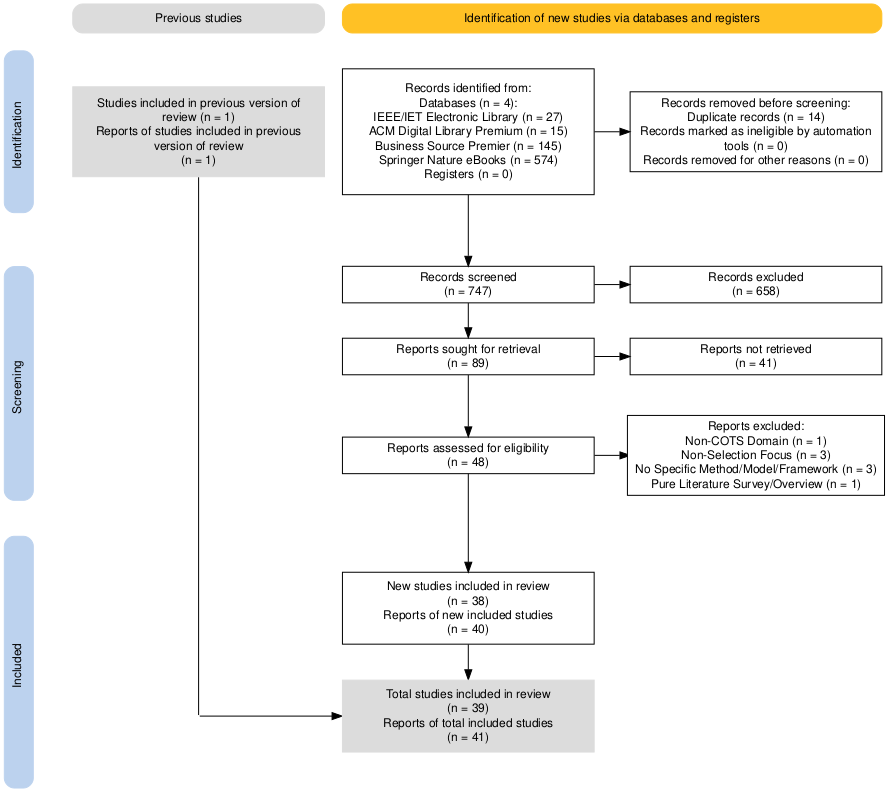
\includegraphics[width=0.82\textwidth]{appendix/prisma_flowchart.png}
  \caption{PRISMA-2020-Flussdiagramm des Such- und Selektionsprozesses \parencite[erstellt über][]{MQ9M8Q7L}}
  \label{fig:prisma_flowchart}
\end{figure}

Wie in Abbildung~\ref{fig:prisma_flowchart} visualisiert, gliederte sich der Selektionsprozess in drei aufeinander aufbauende Stufen:
\begin{enumerate}[label=\textbf{Stufe \arabic*:}, leftmargin=*]
  \item \textbf{Practical Screen 1 (Metadaten-Screening):} Alle 745 Datensätze wurden gegen formale Kriterien geprüft. Ausgeschlossen wurden 597 Publikationen, deren Erscheinungsjahr vor 2000 lag, die nicht in englischer oder deutscher Sprache verfasst waren, reine Vorworte, Konferenz-Inhaltsverzeichnisse oder Editorials darstellten oder keinen fachlichen Bezug zu kommerzieller Standardsoftware aufwiesen. Nach diesem formalen Filter verblieben 148 Publikationen.
  \item \textbf{Practical Screen 2 (Thematisches Relevanz-Screening):} Die 148 Publikationen wurden auf Basis von Titel, Abstract und Schlagwörtern einer Relevanzbewertung auf einer Skala von 1 bis 10 unterzogen. Als Einschlusskriterium galt ein Schwellenwert von $\text{Score} > 7$. Insgesamt wurden 61 Arbeiten exkludiert, die sich primär mit allgemeinen Software-Entwicklungsmethoden im Component-Based Software Engineering (CBSE) ohne Beschaffungs- oder Auswahlsituation befassten, reine Hardware- oder Telekommunikationsinfrastrukturen betrafen oder rein deskriptive Anforderungslisten ohne Entscheidungsmodell diskutierten. 87 Publikationen qualifizierten sich als hochrelevant; unter Berücksichtigung zweier methodischer Grenzfälle wurden 89 Volltexte zur Beschaffung angefordert.
  \item \textbf{Practical Screen 3 (Volltextbeschaffung und Eligibility-Screening):} Von den 89 angeforderten Volltexten konnten über die Hochschullizenzen der DHBW CAS sowie Open-Access-Zugriff 46 Volltexte erfolgreich abgerufen werden. 43 Volltexte waren aufgrund geschlossener fehlender Hochschullizenzen nicht zugänglich (\textit{not retrieved}). Die 46 beschafften Volltexte wurden einer vollständigen inhaltlichen Prüfung gegen die definierten hierarchischer Ausschlusskriterien unterzogen. Acht Volltexte wurden dadurch exkludiert:
  \begin{itemize}[leftmargin=*]
    \item \textit{Ausschlussgrund 1.1 (Non-COTS Domain, $N = 1$):} Der Fokus lag ausschließlich auf der physischen Hardware- und Netzwerkauswahl.
    \item \textit{Ausschlussgrund 1.2 (Non-Selection Focus, $N = 3$):} Die Arbeiten behandelten keine Auswahlsituationen.
    \item \textit{Ausschlussgrund 2.1 (No Specific Method/Model/Framework, $N = 3$):} Reine konzeptionelle Diskussionen oder abstrakte Management-Empfehlungen ohne operationalisiertes mathematisches oder prozedurales Bewertungsmodell.
    \item \textit{Ausschlussgrund 2.2 (Pure Literature Survey / Overview, $N = 1$):} Sekundäre Übersichtsarbeit ohne eigenständigen methodischen Beitrag.
  \end{itemize}
\end{enumerate}

Eine zentrale Publikation wurde aus der Proposal-Recherche integriert, bei der es sich um das COTS-ESF Framework von \textcite{WZM7DUBY} handelt. Die finale Literatursammlung umfasst somit exakt 39 Publikationen (\textit{Reports}), welche 38 unabhängige Primärstudien (\textit{Studies}) repräsentieren, da die Publikationen von \textcite{ZQMG69VT} und \textcite{MZ8JHDYA} als zusammengehöriges Forschungscluster bewertet werden.

\subsubsection{Demografische und bibliometrische Struktur der Literatursammlung}
\label{subsubsec:demografie_korpus}

Die bibliometrische Analyse der Literatursammlung über den Zeitraum 2000 bis 2026 zeigt eine kontinuierliche wissenschaftliche Befassung mit der COTS-Auswahlproblematik. Tabelle~\ref{tab:demografie_qa_uebersicht} fasst die demografischen Kernkennzahlen, Publikationskanäle und Quality-Appraisal-Ergebnisse zusammen.

\begin{table}[htbp]
  \centering
  \small
  \caption{Aggregierte demografische Kennzahlen und Qualitätsverteilung ($N = 39$)}
  \label{tab:demografie_qa_uebersicht}
  \begin{tabularx}{\textwidth}{>{\bfseries\raggedright\arraybackslash}p{3.2cm}>{\raggedright\arraybackslash}Xcc}
    \toprule
    Dimension & Primäre Kategorien im Korpus & Studien ($N$) & Anteil (\%) \\
    \midrule
    Publikationszeitraum & 2000--2009 / 2010--2019 / 2020--2026 & 16 / 13 / 10 & 41,0\,\% / 33,3\,\% / 25,6\,\% \\
    Publikationsorgan & Fachzeitschriften / Konferenzen / Monographien & 21 / 14 / 4 & 53,8\,\% / 35,9\,\% / 10,3\,\% \\
    Evidenzklasse (QA) & Hohe Evidenz (6--8 P.) / Mittlere (3--5 P.) / Niedrig & 36 / 2 / 1 & 92,3\,\% / 5,1\,\% / 2,6\,\% \\
    \midrule
    \multicolumn{4}{p{\dimexpr\textwidth-2\tabcolsep\relax}}{\textbf{Mittelwerte:} QA1: 1,87 \quad QA2: 1,87 \quad QA3: 1,56 \quad QA4: 1,56 \quad \textbf{Gesamt-Mittelwert: 6,87 / 8,00 P.}} \\
    \bottomrule
  \end{tabularx}
\end{table}

In der Dekade 2000--2009 erschienen 16 Publikationen (41,0\,\%). Diese Pionierphase war geprägt von der Etablierung erster Outranking- und AHP-Modelle sowie dem Entwurf dedizierter Software-Werkzeuge. In der zweiten Dekade (2010--2019) wurden 13 Publikationen (33,3\,\%) publiziert, in denen die mathematische Optimierung, nicht-lineare Programmierung und Fuzzy-MCDA-Verfahren dominierten. Die jüngste Phase (2020--2026) steuert 10 Publikationen (25,6\,\%) bei, die sich auf kompositionelle Datenanalysen, Evidential Reasoning und großangelegte Meta-Synthesen konzentrieren.

Hinsichtlich der Publikationsorgane stellen internationale Fachzeitschriften mit 53,8\,\% ($N = 21$) den Hauptanteil dar. Darunter befinden sich renommierte Journals wie \textit{Information Systems Frontiers} \parencite{FCYW9EWJ}, \textit{Information and Software Technology} \parencite{8VHUMEKY}, \textit{Applied Intelligence} \parencite{B7ZTQCZZ, JX4RDRDU}, \textit{Software Quality Journal} \parencite{M3B2D3GD}, \textit{Requirements Engineering} \parencite{DAU8NSK8}, \textit{Annals of Operations Research} \parencite{YVWGHAWQ} und \textit{Complex \& Intelligent Systems} \parencite{UFCEV52H}. Konferenzbeiträge umfassen 35,9\,\% ($N = 14$), unter anderem von der \textit{IEEE Asia-Pacific Services Computing Conference} \parencite{MZ8JHDYA} und der \textit{International Conference on Commercial-off-the-Shelf (COTS)-Based Software Systems (ICCBSS)} \parencite{6RNULWVY}. Hinzu kommen vier wegweisende Dissertationen \parencite{ 9F79VAAB, WBGP3ETU, WZM7DUBY, RRU375GB}.

Geografisch und institutionell lassen sich vier globale Forschungsschwerpunkte identifizieren:
\begin{itemize}[leftmargin=*]
  \item \textbf{Nordamerika:} Die University of Calgary (Kanada) formierte mit den Arbeiten von \textcite{CZZ6XQZJ} und \textcite{9F79VAAB} eine führende Gruppe für Multi-Stakeholder-Verhandlungen und architekturzentriertes Mismatch-Handling. In den USA erforschten \textcite{QDUNCXFC} am NASA Langley Research Center sowie University of Virginia probabilistische Bayes-Netze für sicherheitskritische Raumfahrtsysteme, während \textcite{CI86GRRG} und \textcite{6RNULWVY} an der University of Texas at Dallas modellgetriebene Anforderungs- und Fuzzy-Auswahlverfahren entwickelten.
      \item \textbf{Mitteleuropa:} In Österreich etablierten \textcite{ZQMG69VT} und \textcite{MZ8JHDYA} am Secure Business Austria und der Universität Wien interaktive Mehrzieloptimierungs- und Pareto-DSS-Engines. An der TU Wien konzipierten \textcite{8VHUMEKY} das Plato-System zur automatisierten Benchmark-Evaluation. In Deutschland legten \textcite{WBGP3ETU} an der Universität Augsburg und \textcite{RRU375GB} an der Universität Bamberg umfassende Arbeiten zu Make-or-Buy-Strategien und IoT-Plattformen vor.
  \item \textbf{Südeuropa und Skandinavien:} An der Universitat Politècnica de Catalunya prägte \textcite{TLB687YL} zielorientierte Anforderungsmodelle. An der Universität Paris-Dauphine entwickelten \textcite{LZQJ6M4X} und \textcite{M3B2D3GD} frühe Outranking-Verfahren auf Basis der ISO 9126. Am Politecnico di Milano untersuchten \textcite{DAU8NSK8} empirische AHP-Modelle. In Schweden trieben \textcite{JT5X3FIG} an der Blekinge Institute of Technology und \textcite{UK2X9C4W} an der Universität Lund strategische Sourcing-Taxonomien und kompositionelle Datenanalysen voran.
  \item \textbf{Asien (insbesondere Indien):} Eine außergewöhnlich dichte Serie mathematischer Optimierungs- und Fuzzy-MCDA-Arbeiten entstand an der University of Delhi und der Netaji Subhas University of Technology \parencite{VUVLUN85, 6YJHIVHG, P9SATBH5, B7ZTQCZZ, JX4RDRDU, YVWGHAWQ, 8KF4HAZS}, ergänzt durch Arbeiten der Amity University \parencite{DFASRUVC}, des NITIE Mumbai \parencite{U4E7VXQU} und der PDEU Gujarat \parencite{5BBYQCJB}.
\end{itemize}

\subsubsection{Ergebnisse der Qualitätsbewertung}
\label{subsubsec:qa_ergebnisse}

Die vierdimensionale Qualitätsbewertung bescheinigt der Literatursammlung eine exzellente wissenschaftliche Belastbarkeit. Mit einem Gesamtmittelwert von \textbf{6,87 von 8,00 Punkten} erreichen 36 der 39 Publikationen (92,3\,\%) die höchste Evidenzklasse. Zwei Publikationen (5,1\,\%) fallen in die mittlere Evidenzklasse, während lediglich ein früher konzeptioneller Entwurf (2,6\,\%) der niedrigsten Evidenzklasse zugeordnet wurde.

Die Detailanalyse der Einzeldimensionen (jeweils normiert auf 0 bis 2 Punkte) zeigt folgende Ausprägungen:
\begin{itemize}[leftmargin=*]
  \item \textbf{QA1 (Methodische Transparenz und Formalisierung -- Mittelwert: 1,87):} 34 Publikationen erzielten die Maximalpunktzahl von 2 Punkten. Die mathematischen und algorithmischen Modelle -- von AHP-Supermatrizen über nicht-lineare ganzzahlige Optimierungsgleichungen bis hin zu Dempster-Shafer-Evidenzregeln -- sind formelhaft lückenlos und reproduzierbar spezifiziert.
  \item \textbf{QA2 (Transparenz des Kriterienkatalogs -- Mittelwert: 1,87):} Ebenfalls 34 Publikationen legen vollständig strukturierte, hierarchisch gegliederte Kriterienkataloge offen. Lediglich fünf Publikationen beschränken sich auf unvollständige Beispiellisten.
  \item \textbf{QA3 (Empirische Validierung und Evidenzniveau -- Mittelwert: 1,56):} 22 Publikationen (56,4\,\%) weisen eine reale empirische Validierung anhand von Industrie-Fallstudien, Praktiker-Umfragen oder kontrollierten Experimenten auf. 14 Publikationen demonstrieren ihre Algorithmen an synthetischen numerischen Benchmarks, während drei Publikationen rein theoretisch verbleiben.
  \item \textbf{QA4 (Kritische Reflexion von Grenzen und Kontextfaktoren -- Mittelwert: 1,56):} 22 Publikationen diskutieren Limitationen, kognitiven Aufwand, Rechenkomplexität und Validitätsrisiken tiefgründig. 17 Publikationen begnügen sich mit kurzen methodischen Anmerkungen.
\end{itemize}

% ------------------------------------------------------------------------------
% 4.2 Evolutionäre Abbildung der COTS-Auswahlmethoden
% ------------------------------------------------------------------------------
\subsection{Evolutionäre Abbildung der COTS-Auswahlmethoden}
\label{subsec:evolutionaere_abbildung}

Zur Beantwortung von Forschungsfrage 1 rekonstruiert dieser Abschnitt die historische Entwicklungslinie anhand von vier chronologischen Epochen. Alle 39 Publikationen werden nachfolgend in ihren mathematischen, architektonischen und prozeduralen Beiträgen detailliert analysiert und gewürdigt. Tabelle~\ref{tab:evolutionaere_epochen} bietet eine systematische Übersicht über die Epochen, Leitprofile und Zeiträume (die ausführliche Epochenmatrix mit allen Übergangstreibern ist in Anhang~D, Tabelle~\ref{tab:anhang_epochen_matrix}, dokumentiert).

\begin{table}[htbp]
  \centering
  \small
  \caption{Evolutionäre Epochen der COTS-Softwareauswahl (2000--2026)}
  \label{tab:evolutionaere_epochen}
  \begin{tabularx}{\textwidth}{>{\bfseries\raggedright\arraybackslash}p{2.6cm}>{\raggedright\arraybackslash}p{2.8cm}>{\raggedright\arraybackslash}Xcc}
    \toprule
    Epoche & Zeitraum & Zentrales methodisches Paradigma & Studien ($N$) & Anteil \\
    \midrule
    Epoche 1 & 2000 bis 2005 & Outranking- \& AHP-Modelle (ISO 9126) & 10 & 25,6\,\% \\
    Epoche 2 & 2006 bis 2011 & Architektur, Mismatch-Handling \& DSS & 11 & 28,2\,\% \\
    Epoche 3 & 2012 bis 2019 & Mathematische Optimierung \& Fuzzy-MCDA & 12 & 30,8\,\% \\
    Epoche 4 & 2020 bis 2026 & CoDa, Evidential Reasoning \& Synthesen & 6 & 15,4\,\% \\
    \bottomrule
  \end{tabularx}
\end{table}

\subsubsection{Epoche 1 (2000 bis 2005): Grundlegende Outranking- und frühe Mehrkriterien-Frameworks}
\label{subsubsec:epoche1}

Die erste Epoche (2000 bis 2005) markiert den Übergang von rein informellen, intuitiven Beschaffungsentscheidungen zu formalisierten mathematischen und prozeduralen Bewertungsverfahren. Angesichts explodierender Fehlerraten bei der Einführung unternehmensweiter Softwaresysteme bestand das primäre Ziel darin, die Auswahlentscheidung transparent, objektiv und kriteriengeleitet zu gestalten.

Den Beginn markieren Arbeiten aus dem Bereich der europäischen Outranking-Methode. \textcite{LZQJ6M4X} demonstrierten anhand eines realen Beschaffungsprojekts bei Telecom Italia den Einsatz von ELECTRE-TRI zur Vorfilterung und Klassifikation kommerzieller Angebote im Rahmen öffentlicher Ausschreibungen (\textit{Calls for Tenders}). Ihr Ansatz nutzte Konkordanz- und Diskordanzschwellen, um unzureichende Softwarekandidaten über Veto-Regeln auszusortieren. Der fundamentale Vorteil dieses Outranking-Ansatzes lag in seiner Nicht-Kompensatorik: Gravierende Schwächen in funktionalen Kernanforderungen durften nicht durch hervorragende Werte in Nebenkriterien kompensiert werden. Aufbauend auf dieser Arbeit stellten \textcite{M3B2D3GD} die erste formale Verbindung zwischen Outranking-Relationen und dem internationalen Qualitätsstandard ISO/IEC 9126 her. Sie wiesen mathematisch nach, dass naive additive Aggregationen (wie das klassische gewichtete Punktwertmodell WSM) auf ordinalen Qualitätsmetriken unzulässig sind und führten Präferenz- sowie Indifferenzschwellen zur Vermeidung von Fehlinterpretationen ein.

Parallel dazu etablierten sich hierarchische und netzwerkartige Verfahren. \textcite{DAU8NSK8} operationalisierten den Analytic Hierarchy Process (AHP) auf Basis der ISO/IEC 9126 und validierten das Modell empirisch an einer Stichprobe von 42 kommerziellen CRM-Paketen. Sie zeigten, dass AHP Entscheidungsträgern erlaubt, funktionale Eignung, technische Qualität und Kostenstrukturen strukturiert gegeneinander abzuwägen. Da hierarchische Bäume jedoch Wechselwirkungen zwischen Kriterien vernachlässigen, führten \textcite{FCYW9EWJ} den Analytic Network Process (ANP) in die COTS-Evaluation ein. Mittels Supermatrizen bildeten sie wechselseitige Abhängigkeiten zwischen betriebswirtschaftlichen Kernprozessen, bestehender Legacy-Infrastruktur und Softwareattributen formelhaft ab.

Für hochgradig sicherheitskritische Anwendungsdomänen reichten deterministische Bewertungsbäume nicht aus. \textcite{QDUNCXFC} entwickelten für das \textit{Cockpit Avionics Upgrade} (CAU) des NASA Space Shuttles ein probabilistisches Entscheidungsmodell auf Basis von Bayesian Belief Networks (BBN). Durch die Hinterlegung bedingter Wahrscheinlichkeitstabellen (\textit{Conditional Probability Tables}, CPTs) gelang es, extreme Unsicherheiten hinsichtlich Echtzeitfähigkeit, Speicherzuverlässigkeit und Flugzertifizierung kommerzieller Echtzeitbetriebssysteme (RTOS) mathematisch präzise zu modellieren.

Gleichzeitig entstanden erste hybride und anforderungszentrierte Ansätze. \textcite{CI86GRRG} integrierten Fuzzy-Regelsysteme und Adaptive Neuro-Fuzzy Inference Systems (ANFIS), um Unschärfen in Dienstgütemetriken (QoS) von COTS-Komponenten auszugleichen. \textcite{TLB687YL} konzipierte einen leichtgewichtigen zielorientierten Modellierungsansatz auf Basis des $i^*$-Strategic Dependency Models, der relationale Abhängigkeiten zwischen Organisationszielen (\textit{Strategic Dependency}) und Softwarefähigkeiten (\textit{Strategic Rationale}) analysierte. \textcite{CZZ6XQZJ} legten mit NeMo-CoSe ein Verhandlungsmodell vor, das spieltheoretische Win-Win-Konditionen zwischen heterogenen Stakeholder-Gruppen bei der Komponentenauswahl formalisierte.

\subsubsection{Epoche 2 (2006 bis 2011): Architekturintegration, Mismatch-Behandlung und dedizierte DSS-Engines}
\label{subsubsec:epoche2}

Die zweite Epoche (2006 bis 2011) brachte eine entscheidende architektonische Wende hervor. Die wissenschaftliche Gemeinschaft erkannte, dass Standardsoftwarekomponenten isoliert selten perfekt in bestehende Systemlandschaften passen. Der Forschungsschwerpunkt verlagerte sich daher von der reinen Blackbox-Bewertung hin zur aktiven Mismatch-Erkennung, architektonischen Verträglichkeitsprüfung und der Entwicklung eigenständiger Decision Support Systems (DSS).

\textcite{8XNYS4M9} operationalisierten funktionale Diskrepanzen, indem sie auf Basis von ISO/IEC 9126-2 ein formales Messmodell für funktionale Eignung entwickelten. Dieses differenzierte zwischen funktionaler Vollständigkeit (\textit{Completeness}), Adäquatheit (\textit{Adequacy}) und funktionalem Überhang (\textit{Excess}) und balancierte diese Metriken über AHP-Stakeholdergewichte im E-Payment-Kontext. \textcite{6RNULWVY} automatisierten den Anforderungsabgleich im CARE-Framework (\textit{Component-Aware Requirements Engineering}), indem sie syntaktische Baum-Editierdistanzen mit semantischen WordNet-Ontologien kombinierten, um funktionale \enquote{Near-Miss}-Kandidaten über Softgoal Interdependency Graphs (SIG) algorithmisch zu identifizieren. \textcite{U5JPV4SF} präsentierte eine Hybridisierung, die ANP zur Modellierung von Kriterieninterdependenzen mit einem modifizierten TOPSIS-Algorithmus vereinte, um Workflow-Management-Systeme anhand euklidischer Distanzen zu idealen Referenzpunkten zu bewerten.

Einen Meilenstein setzte die Dissertation von \textcite{9F79VAAB}, der das MiHOS-Framework (\textit{Mismatch Handling aware COTS Selection}) schuf. Mohamed systematisierte funktionale, architektonische und nicht-funktionale Inkompatibilitäten in einer fundierten Taxonomie und integrierte die mathematische Planung von Anpassungsmaßnahmen (z.\,B. Glue-Code, Wrapper-Synthese) direkt in das Auswahl-DSS, begleitet durch die neuartige Sensitivitätsanalyse IDS-SA.

Parallel dazu revolutionierten \textcite{ZQMG69VT} und \textcite{MZ8JHDYA} die multikriterielle Entscheidungsfindung: Anstatt Entscheidungsträger zu zwingen, Kriteriengewichte \textit{a priori} festzulegen -- was bei unvollständiger Marktkenntnis regelmäßig zu Fehlentscheidungen führt -- formulierten sie das Auswahlproblem als multikriterielle 0-1-Ganzzahlprogrammierung. In ihrem interaktiven DSS-Werkzeug Atana/Odin erkunden Entscheidungsträger interaktiv die Pareto-optimale Lösungsfront. Dadurch wird kognitive Überlastung vermieden und Portfolio-Kombinationen werden ohne a-priori-Gewichtsverzerrungen identifiziert, wie die Validierung im österreichischen Sozialversicherungssektor (MediCorp-Fallstudie) belegte.

Weitere spezialisierte DSS-Artefakte entstanden in dieser Phase: \textcite{8VHUMEKY} entwickelten das Plato-DSS für digitale Langzeitarchivierung, das subjektive Experteneinschätzungen durch vollautomatisierte empirische Benchmark-Messreihen und objektive Nutzenbäume ersetzte. \textcite{VUVLUN85} formulierten ein nicht-lineares 0-1-Optimierungsmodell zur Komponentenauswahl unter fehlertoleranten \textit{Recovery Block} (RB) Architekturen, das Zuverlässigkeit, Kosten und Ausführungszeit simultan optimierte. \textcite{WBGP3ETU} strukturierte die strategische Make-or-Buy-Entscheidung architektonisch, während \textcite{U4E7VXQU} mit HKBS ein wissensbasiertes System schufen, das regelbasierte Vorabfilterung, fallbasiertes Schließen (\textit{CBRank}) und AHP vereinte.

\subsubsection{Epoche 3 (2012 bis 2019): Mathematische Optimierung und Ausbreitung von Fuzzy-MCDA}
\label{subsubsec:epoche3}

Die dritte Epoche (2012--2019) war durch eine massive Mathematisierung und die Ausbreitung der Fuzzy-Set-Theorie gekennzeichnet. Die Wissenschaftliche Gemeinschaft reagierte damit auf die Erkenntnis, dass Expertenurteile bei komplexen Softwarebeschaffungen naturgemäß vage, linguistisch geprägt und mit erkenntnistheoretischer Unsicherheit behaftet sind.

\textcite{6YJHIVHG} formulierten ein interaktives Fuzzy-Mathematisches Programmierungsmodell (FMP), das ISO-9126-Qualitätsmetriken in eine simultane Optimierung von Kosten, Zuverlässigkeit, Lieferzeit und Ausführungszeit modularer Systeme einbettete. \textcite{W8P543Y2} erweiterten MCDM-Systeme für Cloud-basierte SaaS-ERP-Systeme um dynamische QoS-Messungen und Social-Network-Reputationsbewertungen. \textcite{VRTXHQI7} entwickelten ein hybrides Fuzzy-MCDA-Modell für CAD/CAM-Software, das die relative Nähe zur idealen Lösung via Fuzzy-TOPSIS mit den nicht-kompensatorischen Veto-Schwellen von Fuzzy-ELECTRE kombinierte.

\textcite{WZM7DUBY} entwickelte in seiner Dissertation das COTS-ESF-Framework, das AHP-Gewichtungen mathematisch mit quantitativer Gap-Analyse verknüpfte, um Anpassungsaufwände und Schnittstellenrisiken vor der Kaufentscheidung formelhaft zu quantifizieren. \textcite{LYMHTPXS} operationalisierten die neu verabschiedete Qualitätsnorm ISO/IEC 25010 für ein gewichtetes Attribut-Scoring proprietärer und quelloffener BPMS-Werkzeuge.

Eine Serie mathematisch hochgradig anspruchsvoller Arbeiten stammte von der Forschergruppe um Gupta, Mehlawat, Jha und Verma: \textcite{P9SATBH5} modellierten die Komponentenauswahl unter einem fehlertoleranten \textit{Consensus Recovery Block} (CRB) Schema mittels Fuzzy-Nichtlinearer Optimierung in LINGO. \textcite{B7ZTQCZZ} kombinierten Fuzzy-TOPSIS mit kompensatorischen Credibility-Chance-Constrained-Modellen, während \textcite{JX4RDRDU} ein multikriterielles kredibilistisches 0-1-Programmierungsmodell vorlegten, das Erwartungswert- und Zufallsparameter unter Fuzzy-Glaubwürdigkeitsmaßen simultan steuerte.

Ergänzt wurde diese Phase durch hierarchische Wiederverwendungsmodelle von \textcite{DFASRUVC}, das strategische GRADE-Sourcing-Framework von \textcite{JT5X3FIG}, die methodische Triangulation aus Delphi-Filterung, Fuzzy-AHP und PROMETHEE-II-Outranking-Flüssen von \textcite{NZJEEPAC} sowie die Usability-fokussierte AHP-VIKOR-Kompromissrangbildung von \textcite{QNWK8SAP}.

\subsubsection{Epoche 4 (2020 bis 2026): Kompositionelle Daten, Evidential Reasoning und Meta-Analysen}
\label{subsubsec:epoche4}

Die jüngste Epoche (2020 bis 2026) zeichnet sich durch methodische Reifung, die Beseitigung struktureller mathematischer Verzerrungen klassischer Verfahren sowie breit angelegte empirische und methodische Meta-Analysen aus.

Einen herausragenden methodenkritischen Beitrag leisteten \textcite{UK2X9C4W}: Sie wiesen mathematisch nach, dass traditionelle Punkteverteilungsverfahren wie das Cumulative Voting (\$100-Test) aufgrund der konstanten Summenrestriktion im Simplex-Raum massiven statistischen Scheinkorrelationen unterliegen. Durch die Einführung der \textit{Compositional Data Analysis} (CoDa) mit Centered Log Ratio (CLR) Transformationen etablierten sie ein verzerrungsfreies statistisches Fundament zur Priorisierung von ISO/IEC-25010-Qualitätsattributen, validiert an 157 Software-Praktikern.

\textcite{5BBYQCJB} validierten empirisch ein Fuzzy-AHP-Modell mit Dreiecks-Fuzzy-Zahlen zur ERP-Auswahl in Industrieunternehmen. \textcite{UFCEV52H} führten das Konzept der \textit{Fuzzy Intra-Coupling Density} (Fuzzy-ICD) in ein nicht-lineares 0-1-Ganzzahlmodell ein, um modulare Kopplungen und Kohäsionen in Build-or-Buy-Architekturen simultan mit Kosten und Zuverlässigkeit zu optimieren.

Einen Höhepunkt der Evidenzkonsolidierung bildet die 588-seitige DSR-Monographie von \textcite{RRU375GB}, die in einer Meta-Analyse von 139 COTS-Publikationen den State-of-the-Art systematisierte und einen ganzheitlichen Kriterienkatalog sowie eine Referenzarchitektur für IoT-Softwareplattformen entwickelte. \textcite{FVINCQ89} präsentierte den FMDBA-Ansatz (\textit{Fuzzy Modified Distance-Based Approach}), der subjektive Expertengewichte mit objektiver Fuzzy-Entropie fusionierte. \textcite{YVWGHAWQ} verknüpften die Effizienzgrenzen der Data Envelopment Analysis (DEA) mit evolutionären NSGA-II-Algorithmen zur Komponentenauswahl unter optimaler Redundanz. \textcite{8KF4HAZS} etablierten ein Zwei-Phasen-Framework aus Fuzzy-TOPSIS und interaktiver Optimierung für Multi-Applikations-Suiten.

Einen wegweisenden Schritt zur Behandlung erkenntnistheoretischer Unvollständigkeit vollzog \textcite{LNQHES84} durch den Einsatz des Evidential Reasoning (ER) auf Basis der Dempster-Shafer-Theorie. Dieses Modell erlaubt es, unvollständige Anbieterauskünfte und konfligierende Gutachterbewertungen über Glaubensverteilungen (\textit{Belief Distributions}) und Nichtwissensgrade mathematisch exakt abzubilden. Schließlich lieferten \textcite{LPC92LAP} eine kritische Meta-Analyse über 41 Arbeiten zum Einsatz von MCDM im Software Engineering, in der sie Phänomene der Rangumkehr (\textit{Rank Reversal}) und kognitive Überlastungen beleuchteten.

% ------------------------------------------------------------------------------
% 4.3 Morphologische Analyse der COTS-Auswahlmethoden
% ------------------------------------------------------------------------------
\subsection{Morphologische Analyse der COTS-Auswahlmethoden}
\label{subsec:morphologische_analyse_ergebnisse}

Zur Beantwortung von Forschungsfrage 2 wird die in Abschnitt~\ref{subsec:morphologische_analyse_methodik} hergeleitete General Morphological Analysis (GMA) nach Zwicky und Ritchey \parencite[S.~81 bis 91]{Z6N6V5L9} empirisch auf die Literatursammlung angewendet.

\subsubsection{Induktive Konstruktion des morphologischen Feldes}
\label{subsubsec:feldkonstruktion}

Die sechs Schlüsselparameter ($P_1 \dots P_6$) und ihre diskreten Ausprägungen wurden induktiv und theoriegeleitet aus den Merkmalen der 17-spaltigen Datenextraktionsmatrix (Abschnitt~\ref{subsec:qualitaetsbewertung_datenextraktion}) abgeleitet. Sie erfüllen die formalen Bedingungen der Parameter-Orthogonalität (wechselseitiger Ausschluss) und kollektiven Erschöpfung \parencite[vgl.][S.~82 bis 83]{Z6N6V5L9}:
\begin{enumerate}[label=\textbf{\arabic*.}, leftmargin=*]
  \item \textbf{$P_1$ (Mathematisches Entscheidungs- und Gewichtungsmodell):} Operationalisiert das fundamentale mathematische Paradigma aus den Extraktionsfeldern \\ \texttt{Mathematical\_Decision\_Model} und \texttt{Primary\_Methodological\_Approach}. Es umfasst $|P_1| = 6$ disjunkte Ausprägungen: klassische MCDA ($v_{1.1}$), Outranking ($v_{1.2}$), mathematische Optimierung ($v_{1.3}$), Fuzzy-MCDA/OR ($v_{1.4}$), probabilistische/wissensbasierte KI ($v_{1.5}$) und rein qualitative/zielorientierte Modelle ($v_{1.6}$).
  \item \textbf{$P_2$ (Entscheidungsunterstützungs-Automatisierung):} Erfasst den werkzeugtechnischen Reifegrad aus dem Feld \texttt{Decision\_Support\_Automation} mit $|P_2| = 3$ Ausprägungen: manuelle Leitfäden ($v_{2.1}$), Solver/Skripte/Tabellenkalkulationen ($v_{2.2}$) und vollwertige interaktive Decision Support Systems mit GUI ($v_{2.3}$).
  \item \textbf{$P_3$ (Mismatch- und Inkompatibilitätsbehandlung):} Systematisiert die architektonische Integrationsfähigkeit aus den Feldern \texttt{Mismatch\_Handling} und \\ \texttt{Mismatch\_Handling\_Phase} mit $|P_3| = 4$ Ausprägungen: keine Behandlung ($v_{3.1}$), Vorabfilterung ($v_{3.2}$), mathematische Nebenbedingungen ($v_{3.3}$) und post-selektive Adaptationsplanung inklusive Schnittstellen-/Wrapper-Kosten ($v_{3.4}$).
  \item \textbf{$P_4$ (Unsicherheits- und Unschärfemodellierung):} Klassifiziert den mathematischen Umgang mit epistemischer und stochastischer Vagheit aus dem Feld \\ \texttt{Uncertainty\_Handling} mit $|P_4| = 4$ Ausprägungen: deterministische Punktwerte ($v_{4.1}$), Fuzzy-Set-Theorie ($v_{4.2}$), Sensitivitäts-/Intervallanalysen inklusive CoDa ($v_{4.3}$) und probabilistische Bayes-/Evidenztheorie ($v_{4.4}$).
  \item \textbf{$P_5$ (Umfang des Kriterienkatalogs):} Bildet die inhaltliche Bewertungsbreite aus dem Feld \texttt{Covered\_Criteria\_Types} mit $|P_5| = 3$ Ausprägungen ab: rein funktionale Eignung ($v_{5.1}$), Softwarequalität und Performance ($v_{5.2}$) sowie ganzheitlich-mehrdimensionale Kriterienbäume ($v_{5.3}$).
  \item \textbf{$P_6$ (Kriterien-Standardisierung und Wiederverwendbarkeit):} Erfasst den Grad der normativen Verankerung aus dem Feld \texttt{Criteria\_Catalog\_Structure} mit $|P_6| = 3$ Ausprägungen: ad-hoc generiert ($v_{6.1}$), standardbasiert nach ISO/IEC 9126 bzw. ISO/IEC 25010 ($v_{6.2}$) und wiederverwendbare Ontologien bzw. Wissensbasen ($v_{6.3}$).
\end{enumerate}

Das kartesische Produkt der Parameterdomänen spannt einen theoretischen Gesamtraum von
\begin{equation}
  N = \prod_{i=1}^{6} |P_i| = 6 \times 3 \times 4 \times 4 \times 3 \times 3 = 2.592 \text{ Konfigurationen} \notag
\end{equation}
auf. Tabelle~\ref{tab:morphologisches_feld} fasst die sechs Dimensionen des morphologischen Feldes zusammen (das vollständige morphologische Feld mit allen 25 diskreten Ausprägungen und Definitionen ist in Anhang~F, Tabelle~\ref{tab:anhang_morphologisches_feld}, dokumentiert).

\begin{table}[htbp]
  \centering
  \small
  \caption{Übersicht der sechs morphologischen Dimensionen ($N = 2.592$ Konfigurationen)}
  \label{tab:morphologisches_feld}
  \begin{tabularx}{\textwidth}{cl>{\raggedright\arraybackslash}Xcc}
    \toprule
    \textbf{ID} & \textbf{Morphologischer Parameter} & \textbf{Dominante Ausprägung im Korpus} & \textbf{$N$} & \textbf{Anteil} \\
    \midrule
    $P_1$ & Mathematisches Entscheidungsmodell & Fuzzy-MCDA \& Fuzzy-OR ($v_{1.4}$) & 11 & 28,2\,\% \\
    $P_2$ & Automatisierungsgrad & Skripte, Tabellen \& Solver ($v_{2.2}$) & 21 & 53,8\,\% \\
    $P_3$ & Mismatch-Behandlung & Vorabfilterung ($v_{3.2}$) / Nebenbedingungen ($v_{3.3}$) & je 15 & je 38,5\,\% \\
    $P_4$ & Unsicherheitsmodellierung & Deterministisch ($v_{4.1}$) / Fuzzy-Sets ($v_{4.2}$) & 16 / 13 & 41,0\,\% / 33,3\,\% \\
    $P_5$ & Kriterienkatalog-Umfang & Ganzheitlich mehrdimensional ($v_{5.3}$) & 22 & 56,4\,\% \\
    $P_6$ & Kriterien-Standardisierung & Ad-hoc projektspezifisch generiert ($v_{6.1}$) & 19 & 48,7\,\% \\
    \bottomrule
  \end{tabularx}
\end{table}

\subsubsection{Parameteranalyse des morphologischen Feldes}
\label{subsubsec:parameteranalyse}

Die relative Häufigkeitsverteilung über alle sechs Parameter gliedert sich wie folgt:
\begin{itemize}[leftmargin=*]
  \item \textbf{$P_1$ (Mathematisches Entscheidungs- und Gewichtungsmodell):} Das Feld wird von Fuzzy-MCDA- und Fuzzy-OR-Modellen dominiert ($v_{1.4}$: 28,2\,\%, $N = 11$), gefolgt von klassischen deterministischen MCDA-Ansätzen ($v_{1.1}$: 23,1\,\%, $N = 9$). Qualitative und prozessorientierte Modelle umfassen 17,9\,\% ($v_{1.6}$, $N = 7$), während probabilistische, evidenzbasierte und wissensbasierte Systeme 15,4\,\% stellen ($v_{1.5}$, $N = 6$). Mathematische Optimierungsmodelle ($v_{1.3}$: 10,3\,\%, $N = 4$) und reine Outranking-Verfahren ($v_{1.2}$: 5,1\,\%, $N = 2$) bilden spezialisierte Nischen.
  \item \textbf{$P_2$ (Automatisierungsgrad der Entscheidungsunterstützung):} Mehr als die Hälfte aller Publikationen ($v_{2.2}$: 53,8\,\%, $N = 21$) stützt sich auf mathematische Skripte, Tabellenkalkulationen oder kommerzielle OR-Solver (z.\,B. LINGO, MATLAB). 28,2\,\% ($v_{2.3}$, $N = 11$) implementieren vollwertige interaktive Decision Support Systems mit eigener GUI. 17,9\,\% ($v_{2.1}$, $N = 7$) verbleiben auf Ebene manueller prozeduraler Richtlinien.
  \item \textbf{$P_3$ (Mismatch- und Inkompatibilitätsbehandlung):} Jeweils 38,5\,\% ($N = 15$) nutzen Vorabfilterung ($v_{3.2}$) oder mathematische Nebenbedingungen ($v_{3.3}$). Dagegen adressieren lediglich 10,3\,\% ($v_{3.4}$, $N = 4$) die fundamentale post-selektive Adaptationsplanung (Glue-Code, Gap Analysis). 12,8\,\% ($v_{3.1}$, $N = 5$) ignorieren Mismatches vollständig.
  \item \textbf{$P_4$ (Unsicherheits- und Unschärfemodellierung):} 41,0\,\% ($v_{4.1}$, $N = 16$) arbeiten rein deterministisch mit Einzelwerten. 33,3\,\% ($v_{4.2}$, $N = 13$) modellieren Unschärfe über Fuzzy-Zahlen. Sensitivitätsanalysen und CoDa-Log-Ratios stellen 17,9\,\% ($v_{4.3}$, $N = 7$), während probabilistische Bayes-Netze und Dempster-Shafer-Evidenzmodelle 7,7\,\% umfassen ($v_{4.4}$, $N = 3$).
  \item \textbf{$P_5$ (Umfang des Kriterienkatalogs):} Die Mehrheit ($v_{5.3}$: 56,4\,\%, $N = 22$) verfolgt ganzheitliche Kriterienkataloge (Funktionalität, NFRs, Kosten, Anbieterlebensfähigkeit). 33,3\,\% ($v_{5.2}$, $N = 13$) fokussieren primär Softwarequalität und technische Leistung, während 10,3\,\% ($v_{5.1}$, $N = 4$) rein funktionale Schnittstellen prüfen.
  \item \textbf{$P_6$ (Kriterien-Standardisierung und Wiederverwendbarkeit):} Fast die Hälfte aller Publikationen ($v_{6.1}$: 48,7\,\%, $N = 19$) definiert Kriterien ad-hoc für spezifische Fallbeispiele. 28,2\,\% ($v_{6.3}$, $N = 11$) nutzen wiederverwendbare Taxonomien oder Ontologien, während 23,1\,\% ($v_{6.2}$, $N = 9$) explizit auf ISO/IEC 9126 oder ISO/IEC 25010 referenzieren.
\end{itemize}

\subsubsection{Durchführung und Ergebnisse des Cross-Consistency Assessments (CCA)}
\label{subsubsec:cca_ergebnisse}

Gemäß der wissenschaftstheoretischen Formalisierung der General Morphological Analysis nach \textcite[S.~83 bis 86]{Z6N6V5L9} bildet das Cross-Consistency Assessment (CCA) das methodische Kernstück zur Bereinigung des theoretischen Konfigurationsraums ($N = 2.592$). Da das kartesische Produkt aller Parameterdomänen zahlreiche Kombinationen enthält, die in der Realität mathematisch unzulässig, algorithmisch widersprüchlich oder praktisch nicht umsetzbar sind, wurden alle $\binom{6}{2} = 15$ paarweisen zweidimensionalen Teilmatrizen mit insgesamt 217 disjunkten Zustandspaaren systematisch evaluiert (siehe Tabelle~\ref{tab:cca_uebersicht}; alle 15 detaillierten 2D-Kreuzmatrizen sind in Anhang~E hinterlegt).

\begin{table}[htbp]
  \centering
  \small
  \caption{Ergebnisse des Cross-Consistency Assessments (CCA) über 15 Teilmatrizen}
  \label{tab:cca_uebersicht}
  \begin{tabularx}{\textwidth}{cl>{\raggedright\arraybackslash}Xcc}
    \toprule
    \textbf{Klasse} & \textbf{Status} & \textbf{Methodische Bedeutung} & \textbf{Zellen ($N$)} & \textbf{Anteil} \\
    \midrule
    $O$ & Empirisch beobachtet & Real belegte Methodenkombinationen der Literatur & 168 & 77,4\,\% \\
    $?$ & Plausibel / Unbesetzt & Konsistente theoretische Innovationsräume & 45 & 20,7\,\% \\
    $X$ & Inkompatibel & Formal-logisch oder mathematisch unzulässig & 4 & 1,8\,\% \\
    \midrule
    \multicolumn{3}{l}{\textbf{Gesamtzahl aller evaluierten paarweisen Relationen ($P_A \times P_B$):}} & \textbf{217} & \textbf{100,0\,\%} \\
    \bottomrule
  \end{tabularx}
\end{table}

Wie die aggregierte Auswertung in Tabelle~\ref{tab:cca_uebersicht} verdeutlicht, gliedert sich der morphologische Gesamtraum in drei distinkte Konsistenzklassen:
\begin{enumerate}[label=\textbf{\alph*)}, leftmargin=*]
  \item \textbf{Empirisch beobachtete Konfigurationen ($O$ -- 168 Zellen / 77,4\,\%):} Diese Parameterkombinationen sind in mindestens einer der 39 untersuchten Primärstudien real belegt. Sie spiegeln die etablierten methodischen Entwicklungspfade der letzten 26 Jahre wider und bilden die empirische Basis für die typologische Synthese der vier methodischen Archetypen (Abschnitt~\ref{subsubsec:archetypen_analyse}).
  \item \textbf{Plausible, unbesetzte Innovationsräume ($?$ -- 45 Zellen / 20,7\,\%):} Diese Relationen weisen keinerlei logische, mathematische oder funktionale Widersprüche auf, werden jedoch in der aktuellen COTS-Literatur nicht empirisch adressiert. Sie markieren ungenutzte Synergien und bilden den methodischen Ausgangspunkt für die theoriegeleitete Identifikation der vier zentralen Forschungslücken in Kapitel~\ref{subsec:identifikation_forschungsluecken}.
  \item \textbf{Logisch-strukturelle Inkompatibilitäten ($X$ -- 4 Zellen / 1,8\,\%):} Vier Zellenrelationen wurden aufgrund formaler und axiomatisch unauflösbarer Widersprüche eliminiert:
  \begin{itemize}[leftmargin=*]
    \item \textit{$(P_1 = v_{1.3}) \times (P_2 = v_{2.1})$ (Mathematische Optimierung $\times$ Manuelle Prozesse):} Die nicht-lineare oder ganzzahlige 0-1-Ganzzahlprogrammierung ist NP-schwer und erfordert zwingend algorithmische Gleichungslöser (z.\,B. Branch-and-Bound-Solver in LINGO oder MATLAB); eine rein prozedural-manuelle Abarbeitung ist mathematisch ausgeschlossen.
    \item \textit{$(P_1 = v_{1.5}) \times (P_2 = v_{2.1})$ (KI, Bayes-Netze \& Matching $\times$ Manuelle Prozesse):} Die Berechnung bedingter Wahrscheinlichkeitstabellen (CPTs) in gerichteten azyklischen Graphen (DAGs) sowie ontologiebasierte Baum-Editierdistanzen verlangen zwingend spezialisierte Rechenwerkzeuge.
    \item \textit{$(P_1 = v_{1.4}) \times (P_4 = v_{4.1})$ (Fuzzy-MCDA/OR $\times$ Deterministische Einzelwerte):} Fuzzy-Entscheidungsverfahren basieren per Definition auf unscharfen Zugehörigkeitsfunktionen oder Kredibilitätsverteilungen; die Beschränkung auf rein deterministische Crisp-Einzelwerte hebt das fundamentale mathematische Paradigma auf.
    \item \textit{$(P_2 = v_{2.1}) \times (P_4 = v_{4.4})$ (Manuelle Prozesse $\times$ Probabilistisches \& Evidential Reasoning):} Die exakte Evidenzakkumulation nach Dempster-Shafer mit $2^{|\Theta|}$ Teilmengen und die Modellierung von Nichtwissensgraden $m(\Theta)$ sind ohne computergestützte Werkzeuge fehlerfrei nicht durchführbar.
  \end{itemize}
\end{enumerate}

Die vollständige tabellarische Dokumentation aller 15 paarweisen Kreuzmatrizen samt der zitatbasierten Begründungen für jede einzelne Zellenrelation ist aus Gründen der wissenschaftlichen Transparenz und Intersubjektivität lückenlos in Anhang~E hinterlegt.

\subsubsection{Vergleichende Analyse der vier methodischen Archetypen}
\label{subsubsec:archetypen_analyse}

Durch Gruppierung der diskreten 6-Tupel-Profile lassen sich alle 39 Publikationen vier methodischen Archetypen zuordnen, deren Eigenschaften in Tabelle~\ref{tab:archetypen_matrix} gegenübergestellt sind (die detaillierte Vergleichsmatrix mit Stärken und Grenzen ist in Anhang~G, Tabelle~\ref{tab:anhang_archetypen_matrix}, dokumentiert).

\begin{table}[htbp]
  \centering
  \small
  \caption{Übersicht der vier synthetisierten methodischen Archetypen}
  \label{tab:archetypen_matrix}
  \begin{tabularx}{\textwidth}{>{\bfseries\raggedright\arraybackslash}p{2.8cm}>{\raggedright\arraybackslash}p{3.2cm}>{\raggedright\arraybackslash}Xcc}
    \toprule
    Archetyp & Leitmethoden & Kerncharakteristik & Studien ($N$) & Anteil \\
    \midrule
    Archetyp 1 & AHP, ANP, ELECTRE, WSM & Transparente Kriterien \& ISO-Normbezug & 17 & 43,6\,\% \\
    Archetyp 2 & 0-1 IP, DEA, Multi-Obj. & Globale portfolio-weite Systemoptimierung & 4 & 10,3\,\% \\
    Archetyp 3 & Fuzzy-AHP, Fuzzy-TOPSIS & Modellierung epistemischer Unschärfe & 11 & 28,2\,\% \\
    Archetyp 4 & DSS, BBN, ER, Plato & Interaktive Tools \& Mismatch-Adaptation & 7 & 17,9\,\% \\
    \bottomrule
  \end{tabularx}
\end{table}


\begin{enumerate}[label=\textbf{\arabic*.}, leftmargin=*]
  \item \textbf{Archetyp 1: Classic \& Outranking Decision Engineering ($N = 17$ Publikationen):}  
  Dieser Archetyp repräsentiert traditionelle multikriterielle Analysemethoden wie AHP, ANP, WSM, ELECTRE und zielorientierte Graphen \parencite[Dazu gehören:][]{LZQJ6M4X, M3B2D3GD, FCYW9EWJ, DAU8NSK8, TLB687YL, CZZ6XQZJ, 8XNYS4M9, U5JPV4SF, WBGP3ETU, WZM7DUBY, LYMHTPXS, DFASRUVC, JT5X3FIG, QNWK8SAP, UK2X9C4W, RRU375GB, LPC92LAP}.  
  \textit{Stärken:} Höchste methodische Transparenz, direkte Abbildbarkeit auf Standard-Qualitätsmodelle (ISO/IEC 9126 und 25010) sowie effektive Veto-Mechanismen gegen K.-o.-Kriterien.  
  \textit{Grenzen:} Extreme kognitive Belastung bei Paarvergleichen ($n(n-1)/2$), Anfälligkeit für das Phänomen der Rangumkehr (\textit{Rank Reversal}) bei nachträglichem Hinzufügen oder Entfernen von Alternativen sowie eine rein statische Vorabfilterung von Mismatches.
  
  \item \textbf{Archetyp 2: Multi-Objective Mathematical Programming \& Optimization ($N = 4$ Publikationen):}  
  Hierunter fallen ganzzahlige und nicht-lineare mathematische Optimierungsmodelle des Operations Research \parencite[Dazu gehören:][]{ZQMG69VT, MZ8JHDYA, VUVLUN85, YVWGHAWQ}.  
  \textit{Stärken:} Ganzheitliche globale Systemoptimierung modularer Architekturen; simultane Einhaltung von Budget-, Lieferzeit- und Zuverlässigkeitsgrenzen; formale Modellierung von Redundanzallokationen (z.\,B. Recovery Blocks) und architektonischen Verträglichkeitsmatrizen.  
  \textit{Grenzen:} Hohe Sensitivität gegenüber der Formulierung von Zielfunktionen; Abhängigkeit von teuren kommerziellen Solvern; primäre Verwendung ad-hoc generierter Kriterien ohne Anbindung an internationale Software-Qualitätsnormen.
  
  \item \textbf{Archetyp 3: Fuzzy \& Credibilistic Decision Systems ($N = 11$ Publikationen):}  
  Dieser Archetyp umfasst Modelle, die Unschärfe und vage Expertenpräferenzen über Dreiecks- oder Trapezzahlen, linguistische Skalen oder kredibilistische Zufallsrestriktionen steuern \parencite[Dazu gehören:][]{CI86GRRG, 6YJHIVHG, VRTXHQI7, P9SATBH5, B7ZTQCZZ, JX4RDRDU, NZJEEPAC, 5BBYQCJB, UFCEV52H, FVINCQ89, 8KF4HAZS}.  
  \textit{Stärken:} Exzellente Abbildung epistemischer Vagheit; Vermeidung künstlicher Schwellenwert-Sprünge an Eignungsgrenzen; robuste Kompromissbildung.  
  \textit{Grenzen:} Hoher mathematischer Defuzzifizierungsaufwand; \enquote{Black-Box}-Wirkung auf betriebliche Entscheidungsträger; praktische Umsetzung fast ausschließlich in akademischen Skripten ohne benutzerfreundliche Oberflächen.
  
  \item \textbf{Archetyp 4: Interactive, Intelligent \& Architecture-Aware Decision Support ($N = 7$ Publikationen):}  
  Die methodische Speerspitze bilden integrierte, intelligente DSS-Umgebungen \parencite[Dazu gehören:][]{QDUNCXFC, 6RNULWVY, 9F79VAAB, 8VHUMEKY, U4E7VXQU, W8P543Y2, LNQHES84}.  
  \textit{Stärken:} Vollständig integrierte Software-Werkzeuge ($v_{2.3}$); explizite Modellierung post-selektiver Integrationsmaßnahmen (Glue-Code, Adapter, Wrapper-Synthese); maschinelle Wissenswiederverwendung über Fallbasen (CBR), Dempster-Shafer-Evidenzfusion und automatisierte Messreihen.  
  \textit{Grenzen:} Sehr hoher initialer Aufwand zur Wissensakquisition und Ontologieerstellung; Gefahr des \enquote{Prototypen-Friedhofs}, da akademische DSS-Werkzeuge nach Projektende selten zu wartbaren Industrie- oder Open-Source-Tools weiterentwickelt werden.
\end{enumerate}

\subsubsection{Vertiefte methodische Kompromisse und praktische Anwendungsbarrieren}
\label{subsubsec:tradeoffs_barrieren}

Die vergleichende Analyse über alle Archetypen hinweg offenbart drei fundamentale methodische Zielkonflikte, die den praktischen Einsatz von COTS-Auswahlmethoden in der Unternehmenspraxis maßgeblich determinieren:

\begin{enumerate}[label=\textbf{\arabic*.}, leftmargin=*]
  \item \textbf{Kognitive Last versus mathematische Expressivität:}  
  Klassische hierarchische Verfahren (insbesondere AHP in Archetyp 1) leiden unter einem kombinatorischen Skalierungsproblem. Bei einem Kriterienbaum mit 20 Subkriterien und 5 Alternativen erfordert der vollständige Paarvergleich $20 \times \frac{5 \times 4}{2} + \frac{20 \times 19}{2} = 200 + 190 = 390$ Einzelbewertungen. In der Praxis führt dies zu rascher kognitiver Ermüdung der Gutachter und gravierenden Inkonsistenzen (Konsistenzverhältnis $\text{CR} > 0,10$). Zwar mindern Fuzzy-Verfahren (Archetyp 3) linguistische Härten, erhöhen jedoch die algorithmische Intransparenz derart, dass Entscheidungsträger die Resultate aufgrund des Black-Box-Charakters ablehnen. Neuere statistische Ansätze wie die kompositionelle Datenanalyse (CoDa nach \parencite{UK2X9C4W}) und distanzbasierte Entropieverfahren \parencite{FVINCQ89} bieten hier vielversprechende Auswege zur Reduktion von Verzerrungen ohne kognitive Überlastung.
  
  \item \textbf{A-priori-Gewichtung versus interaktive Pareto-Exploration:}  
  Ein fundamentaler Schwachpunkt klassischer MCDA-Verfahren besteht im Zwang zur \textit{a-priori}-Festlegung von Kriteriengewichten, bevor die tatsächlich am Markt verfügbaren Softwareeigenschaften im Detail bekannt sind. Wie \textcite{MZ8JHDYA} im MediCorp-Projekt empirisch nachwiesen, führt das unreflektierte Festhalten an starren a-priori-Gewichten regelmäßig dazu, dass hochattraktive Softwarepakete verworfen werden, nur weil sie ein einzelnes, theoretisch hoch gewichtetes Kriterium knapp verfehlen. Die interaktive Mehrzieloptimierung (Archetyp 2 und 4) bricht dieses Paradigma auf: Durch die algorithmische Generierung Pareto-optimaler Lösungsfronten können Entscheidungsträger Kompromisse zwischen Budget, Funktionsabdeckung und Lieferzeit dynamisch visualisieren und explorieren.
  
  \item \textbf{Isolierte Produktauswahl versus architektonische Systemintegration:}  
  Die gravierendste praktische Barriere in der gesamten Literatursammlung ist das \enquote{Integrationsrisiko}. Fast 90\,\% aller untersuchten Methoden (Archetypen 1 bis 3) behandeln die COTS-Auswahl als isolierten Einkaufsakt ($v_{3.1}$ bis $v_{3.3}$), bei dem Mismatches lediglich zum Ausschluss führen. In der industriellen Realität ist jedoch kein COTS-Paket vollkommen mismatch-frei. Ansätze, die den Lebenszyklus nach der Auswahl ignorieren, verursachen exorbitante Folgekosten bei der Implementierung. Nur hochentwickelte architekturzentrierte Frameworks wie MiHOS \parencite{9F79VAAB}, COTS-ESF \parencite{WZM7DUBY} und Plato \parencite{8VHUMEKY} (Archetyp 4) quantifizieren den Aufwand für Glue-Code, Adapter-Entwicklung und architektonische Refaktorisierungen im Vorfeld und binden diese mathematisch in die Gesamtentscheidung ein.
\end{enumerate}

Die hier identifizierten Archetypen, Parameterverteilungen und Kompromisse bilden das methodische Fundament für die in Kapitel~5 folgende vergleichende Diskussion sowie die Ableitung einer zukunftsorientierten Forschungsagenda zur Schließung morphologischer Innovationslücken.

% ==============================================================================
% Kapitel 5: Diskussion der Ergebnisse
% ==============================================================================

\section{Diskussion der Ergebnisse}
\label{sec:diskussion_der_ergebnisse}

Aufbauend auf der in Kapitel~\ref{sec:systematische_literaturuebersicht} durchgeführten empirischen und morphologischen Analyse der 39 Publikationen widmet sich dieses  Kapitel der theoriegeleiteten und praxisorientierten Diskussion der Ergebnisse. Die softwaretechnische und betriebswirtschaftliche Auswahl von \textit{Commercial Off-The-Shelf} (COTS) Software stellt Organisationen vor ein hochkomplexes, multidimensionales Entscheidungsproblem. Fehlentscheidungen in diesem Bereich führen in der Unternehmenspraxis regelmäßig zu gravierenden architektonischen Fehlanpassungen (\textit{Architectural Mismatches}), unkontrollierbaren Folgekosten für nachträgliche Anpassungsprogrammierungen (\textit{Glue-Code}), Performanz- und Sicherheitsengpässen sowie fatalen langfristigen Anbieterabhängigkeiten (\textit{Vendor Lock-in}).

Ziel dieses Kapitels ist es, die Beantwortung der drei leitenden Forschungsfragen konsolidiert zusammenzuführen, die durch das morphologische Cross-Consistency Assessment (CCA) aufgedeckten Forschungslücken theorie- und werkzeugbezogen zu durchdringen, handlungsleitende Implikationen für Wissenschaft und Unternehmenspraxis abzuleiten sowie die methodischen Grenzen und Validitätsbedrohungen der Untersuchung transparent zu reflektieren. Die Struktur gliedert sich in vier Abschnitte:
\begin{enumerate}[label=\textbf{\arabic*.}]
  \item \textbf{Abschnitt~\ref{subsec:zusammenfassung_ergebnisse} (Zusammenfassung der Ergebnisse):} Bietet eine integrierte Beantwortung von Forschungsfrage 1 bis 3 und arbeitet die drei übergeordneten Kernergebnisse der Analyse heraus.
  \item \textbf{Abschnitt~\ref{subsec:identifikation_forschungsluecken} (Identifikation von Forschungslücken):} Vollendet die Beantwortung von Forschungsfrage 3 durch eine tiefgründige Analyse der vier identifizierten morphologischen Forschungslücken.
  \item \textbf{Abschnitt~\ref{subsec:implikationen_forschung_praxis} (Implikationen für Forschung und Praxis):} Leitet wissenschaftliche Paradigmenwechsel sowie eine konkrete Entscheidungsmatrix für IT-Architekten und betriebliche Beschaffungsverantwortliche ab.
  \item \textbf{Abschnitt~\ref{subsec:limitationen} (Limitationen):} Reflektiert methodische Recherchegrenzen, Validitätsbedrohungen beim Einsatz generativer Sprachmodelle und Restriktionen der morphologischen Analyse.
\end{enumerate}

% ------------------------------------------------------------------------------
% 5.1 Zusammenfassung der Ergebnisse
% ------------------------------------------------------------------------------
\subsection{Zusammenfassung der Ergebnisse}
\label{subsec:zusammenfassung_ergebnisse}

Die durchgeführte systematische Literaturübersicht liefert auf Basis von 39 methodisch rigoros begutachteten Publikationen (durchschnittlicher Qualitätsbewertungs-Score von \textbf{6,87 von 8,00 Punkten}; 92,3\,\% \textit{Hohe Evidenzklasse}) ein klares, theoriegestütztes Gesamtbild der Forschungslandschaft. Die Beantwortung der drei übergeordneten Forschungsfragen lässt sich wie folgt konsolidieren:

\begin{enumerate}[label=\textbf{\arabic*.}, leftmargin=*]
  \item \textbf{Forschungsfrage 1:} Die historische Rekonstruktion über den 26-jährigen Beobachtungszeitraum (2000 -- 2026) belegt eine tiefgreifende erkenntnistheoretische und mathematische Weiterentwicklung über vier unterscheidbare Epochen:
  \begin{itemize}[leftmargin=*]
    \item \textit{Epoche 1 (2000 -- 2005): Grundlegende Outranking- und Mehrkriterien-Frameworks:} Etablierung erster formaler Bewertungsmodelle (ELECTRE-TRI, AHP, ANP) und normativer Qualitätsbezüge (ISO/IEC 9126) zur Überwindung rein intuitiver Beschaffungsentscheidungen \parencite{LZQJ6M4X, M3B2D3GD, FCYW9EWJ, DAU8NSK8}.
    \item \textit{Epoche 2 (2006 -- 2011): Architekturintegration, Mismatch-Behandlung und DSS-Engines:} Paradigmenwechsel hin zur aktiven architektonischen Verträglichkeitsprüfung, Quantifizierung von Schnittstellendiskrepanzen und interaktiven Pareto-Entscheidungs-systemen (CARE, MiHOS, Atana, Plato) \parencite{6RNULWVY, 9F79VAAB, MZ8JHDYA, 8VHUMEKY}.
    \item \textit{Epoche 3 (2012 -- 2019): Mathematische Optimierung und Fuzzy-MCDA-Verbreitung:} Intensive Mathematisierung zur Modellierung subjektiver linguistischer Vagheit und modularer Systemarchitekturen mittels Fuzzy-TOPSIS, nicht-linearer 0-1-Ganzzahl-programmierung und Credibility Theory \parencite{6YJHIVHG, VRTXHQI7, WZM7DUBY, B7ZTQCZZ, JX4RDRDU}.
    \item \textit{Epoche 4 (2020 -- 2026): Kompositionelle Daten, Evidential Reasoning und Meta-Analysen:} Methodische Reifung durch Beseitigung statistischer Simplex-Verzerrungen via Compositional Data Analysis (CoDa; \textcite{UK2X9C4W}), exakte Erfassung von Nichtwissen via Dempster-Shafer-Evidenztheorie \parencite{LNQHES84} sowie breit angelegte domänenspezifische Meta-Analysen \parencite{RRU375GB, LPC92LAP}.
  \end{itemize}

  \item \textbf{Forschungsfrage 2:} Das morphologische Feld ($N = 2.592$ Konfigurationen) verdichtet die heterogene Methodenlandschaft in vier Archetypen, die spezifische Stärken, Grenzen und Evidenzgrade aufweisen:
  \begin{itemize}[leftmargin=*]
    \item \textit{Archetyp 1 (Classic \& Outranking Decision Engineering, $N = 17$):} Zeichnet sich durch hohe Transparenz und strikte Konformität zu Qualitätsnormen aus, leidet jedoch unter kombinatorischer Paarvergleichslast ($O(n^2)$) und Anfälligkeit für Rangumkehrungen (\textit{Rank Reversal}).
    \item \textit{Archetyp 2 (Multi-Objective Mathematical Programming \& Optimization, $N = 4$):} Ermöglicht die globale portfolio-weite Systemoptimierung modularer CBSD-Architekturen unter Budget-, Latenz- und Redundanzrestriktionen, ist jedoch stark abhängig von kommerziellen OR-Solvern und stützt sich fast ausschließlich auf isolierte Ad-hoc-Kriterien.
    \item \textit{Archetyp 3 (Fuzzy \& Credibilistic Decision Systems, $N = 11$):} Bietet eine überlegene mathematische Handhabung linguistischer Unschärfe von Gutachtern, erzeugt jedoch eine erhebliche kognitive Barriere durch intransparente Defuzzifizierungen (\enquote{Black-Box}-Charakter) und mangelnde benutzerfreundliche Software-Werkzeuge.
    \item \textit{Archetyp 4 (Interactive, Intelligent \& Architecture-Aware DSS, $N = 7$):} Bildet die methodische Speerspitze durch integrierte Software-Werkzeuge ($v_{2.3}$), automatisierte Messreihen und post-selektive Adaptationsplanung (Glue-Code, Wrapper), scheitert in der Praxis jedoch häufig am Phänomen des akademischen \enquote{Prototypen-Friedhofs}.
  \end{itemize}

  \item \textbf{Forschungsfrage 3:} Das Cross-Consistency Assessment deckt fundamentale strukturelle Defizite an den Schnittstellen zwischen Werkzeugautomatisierung, standardisierten Qualitätsmodellen, automatisierter Telemetrie und mathematischer Mismatch-Optimierung auf.
\end{enumerate}

Über diese Einzelfragen hinausgehend lassen sich aus der Gesamtanalyse drei übergreifende Kernergebnisse abstrahieren, welche die gegenwärtige Forschungslage prägen:

\begin{enumerate}[label=\textbf{\Roman*.}]
  \item \textbf{Methodische Spaltung der Forschungslandschaft:} Es existiert eine tiefe Dichotomie zwischen der isolierten Auswahl monolithischer Einzelpakete (z.\,B. ERP- oder CRM-Systeme mittels MCDA/Fuzzy) und der kombinatorischen Portfolio-Optimierung modularer Softwaresysteme (Component-Based Software Development, CBSD, mittels 0-1-Ganzzahlprogrammierung). Während erstere auf standardisierte Kriterienkataloge und Stakeholder-Konsens fokussieren, optimieren letztere mathematisch isolierte Komponentenmengen ohne Rückkopplung an übergeordnete Qualitätsnormen. Beide Forschungsstränge operieren weitgehend isoliert voneinander, wodurch methodische Synergien ungenutzt bleiben.
  \item \textbf{Kluft zwischen mathematischer Theorie und industrieller Anwendbarkeit:} Während die akademische Forschung zunehmend hochkomplexe Formalismen entwickelt (wie mehrdimensionale Fuzzy-Supermatrizen, Kredibilitäts-Zufalls\-restriktionen oder nicht-lineare 0-1-Optimierungsmodelle), scheitert deren Praxistransfer an fehlenden grafischen Benutzeroberflächen, kognitiver Überlastung durch exzessive AHP-Paarvergleiche und dem Mangel an verständlichen Erklärungsmodellen für betriebliche Entscheider. Die Mehrheit der Methoden verharrt in skriptbasierten Solver-Prototypen ($v_{2.2}$: 53,8\,\%), die im industriellen Alltag nicht wartbar sind.
  \item \textbf{Lebenszyklus-Defizit bei der Mismatch-Behandlung:} Nahezu 90\,\% der untersuchten Methoden beschränken sich darauf, architektonische und funktionale Inkompatibilitäten als statische K.-o.-Ausschlussfilter vor der eigentlichen Bewertung zu behandeln ($v_{3.2}, v_{3.3}$). Die betriebswirtschaftlich und softwarearchitektonisch entscheidende Quantifizierung nachgelagerter Adapter-, Wrapper- und Refaktorisierungskosten ($v_{3.4}$) wird im Auswahlzeitpunkt systematisch vernachlässigt, was zu gravierenden Kostenexplosionen bei der Systemeinführung führt.
\end{enumerate}

% ------------------------------------------------------------------------------
% 5.2 Identifikation von Forschungslücken
% ------------------------------------------------------------------------------
\subsection{Identifikation von Forschungslücken}
\label{subsec:identifikation_forschungsluecken}

Die Durchführung des paarweisen Cross-Consistency Assessments (CCA) über alle $\binom{6}{2} = 15$ Teilmatrizen des morphologischen Feldes ($N = 2.592$ formal denkbare Konfigurationen) ermöglichte die mathematisch präzise Isolierung unbesetzter, jedoch methodisch konsistenter und hochgradig relevanter Innovationsräume ($?$). Im Folgenden werden die vier zentralen morphologischen Forschungslücken detailliert analysiert, wodurch Forschungsfrage 3 vollständig und erschöpfend beantwortet wird. Tabelle~\ref{tab:morphologische_luecken} fasst die Lücken, ihre strukturellen Ursachen und die abgeleitete Forschungsagenda zusammen.

\begin{landscape}
\begin{table}[p]
  \centering
  \small
  \caption{Strukturierte Übersicht der identifizierten morphologischen Forschungslücken}
  \label{tab:morphologische_luecken}
  \begin{tabularx}{\linewidth}{>{\raggedright\arraybackslash}p{3.2cm}>{\raggedright\arraybackslash}p{3.8cm}>{\raggedright\arraybackslash}X>{\raggedright\arraybackslash}X>{\raggedright\arraybackslash}p{4.8cm}}
    \toprule
    \textbf{Forschungslücke} & \textbf{Parameter-Kombination} & \textbf{Strukturelles Defizit in der Literatur} & \textbf{Theoretische \& praktische Barriere} & \textbf{Prioritäre Forschungsagenda} \\
    \midrule
    \textbf{1} 
      & $(P_2 = v_{2.3}) \times (P_6 = v_{6.2})$ \newline DSS $\times$ ISO-Norm
      & Vollständiges Fehlen interaktiver Decision Support Systems mit nativer Implementierung der ISO/IEC 25010.
      & DSS-Prototypen nutzen proprietäre Ad-hoc-Bäume ($v_{6.1}$) oder Ontologien ($v_{6.3}$); ISO-Normen verharren in statischen Tabellenkalkulationen ($v_{2.2}$).
      & Entwicklung quelloffener, modularer DSS-Plattformen mit vorkonfigurierten ISO-25010-Messbäumen und dynamischer Gewichtung. \\
    \addlinespace[3pt]
    \textbf{2} 
      & $(P_1 = v_{1.3}) \times (P_3 = v_{3.4})$ \newline OR-Modelle $\times$ Adaptationsplan
      & Mathematische Optimierungsmodelle berücksichtigen keine quantifizierte post-selektive Mismatch- und Glue-Code-Planung.
      & OR-Modelle behandeln Inkompatibilitäten rein als binäre K.-o.-Restriktionen ($C_{ij} \in \{0,1\}$), wodurch anpassbare Komponenten verworfen werden.
      & Formulierung dynamischer mathematischer Modelle, die Komponentenselektion und Wrapper-Entwicklungs\-aufwände simultan ko-optimieren. \\
    \addlinespace[3pt]
    \textbf{3} 
      & $(P_2 = v_{2.3}) \times (P_4 = v_{4.4})$ \newline DSS $\times$ Evidential Reasoning
      & Mangel an interaktiven DSS-Werkzeugen mit grafischer Modellierung unvollständiger Daten via Dempster-Shafer-Theorie.
      & Evidential Reasoning verbleibt auf Ebene akademischer Formeln; keine anwenderfreundlichen GUIs zur Visualisierung von Nichtwissensintervallen.
      & Konzeption webbasierter Evidenz-DSS, die Glaubens- und Plausibilitätsintervalle für Praktiker visuell erfahrbar machen. \\
    \addlinespace[3pt]
    \textbf{4} 
      & $(P_5 = v_{5.2}) \times (P_6 = v_{6.2}) \times (P_2 = v_{2.3})$ \newline NFR $\times$ Norm $\times$ Benchmarking
      & Weitgehende Entkopplung standardisierter Qualitätskataloge von automatisierter, empirischer Telemetrie- und Benchmark-Erhebung.
      & ISO-Kriterien werden primär über subjektive Fragebögen evaluiert; objektive Testbeds (z.\,B. API-Fuzzing, Lasttests) bleiben isoliert.
      & Nahtlose Integration automatisierter CI/CD-Pipelines und CVE-Sicherheitsfeeds in standardbasierte Qualitätsmodelle. \\
    \bottomrule
  \end{tabularx}
\end{table}
\end{landscape}
\FloatBarrier

\subsubsection{Forschungslücke 1: DSS-Tooling versus standardisierte Qualitätsmodelle}
\label{subsubsec:gap1}

Die erste morphologische Lücke resultiert aus der Schnittmenge von dedizierten, interaktiven Entscheidungsunterstützungssystemen ($P_2 = v_{2.3}$) und standardbasierten Qualitätsmodellen ($P_6 = v_{6.2}$). Während 28,2\,\% aller Publikationen ($N = 11$) interaktive Software-Werkzeuge vorstellen und 23,1\,\% ($N = 9$) auf die internationalen Qualitätsnormen ISO/IEC 9126 bzw. ISO/IEC 25010 rekurrieren, existiert in der gesamten Literatursammlung kein einziges interaktives DSS, das die ISO/IEC 25010 nativ, modular konfigurierbar und mit standardisierten Messvorschriften implementiert.

Die Ursachenanalyse offenbart eine methodische Diskrepanz: Akademische DSS-Pionier\-werkzeuge wie CARE \parencite{6RNULWVY}, MiHOS \parencite{9F79VAAB} oder Atana \parencite{MZ8JHDYA} wurden primär als Machbarkeitsnachweise für spezifische algorithmische Konzepte (z.\,B. Anforderungsgraphen, Goal-Trees oder interaktive Pareto-Exploration) entworfen. Sie stützen sich folglich auf isolierte Ad-hoc-Kriterienbäume ($v_{6.1}$) oder proprietäre Ontologien ($v_{6.3}$). Umgekehrt werden standardisierte Qualitätsmodelle in der Forschung fast ausschließlich als statische Checklisten oder im Rahmen einfacher Tabellenkalkulationen und Skripte ($v_{2.2}$) operationalisiert \parencite{M3B2D3GD, DAU8NSK8, LYMHTPXS}. 

Diese Lücke führt in der Praxis zu gravierenden Ineffizienzen: Entscheider müssen Standard-Qualitätskataloge entweder manuell in generische Tabellenkalkulationen überführen oder auf proprietäre Werkzeuge zurückgreifen, deren Kriterienstrukturen nicht mit internationalen Software-Engineering-Standards harmonieren. Zur Schließung dieser Lücke bedarf es der Entwicklung quelloffener, modular erweiterbarer DSS-Plattformen, welche die Haupt- und Subcharakteristika der ISO/IEC 25010 als vordefinierte Messbäume bereitstellen und mit dynamischen, anwendergesteuerten Gewichtungs- und Aggregationsmechanismen verknüpfen.

\subsubsection{Forschungslücke 2: Automatisierte Mismatch-Resolution versus Mathematische Optimierung}
\label{subsubsec:gap2}

Die zweite fundamentale Forschungslücke betrifft die Kombination aus mathematischer Optimierung des Operations Research ($P_1 = v_{1.3}$) und post-selektiver Mismatch- und Adaptationsplanung ($P_3 = v_{3.4}$). Mathematische Programmierungsansätze \parencite{ZQMG69VT, VUVLUN85, B7ZTQCZZ, JX4RDRDU, UFCEV52H, YVWGHAWQ} zeichnen sich durch ihre herausragende Fähigkeit aus, modulare Softwaresysteme unter kombinatorischen Restriktionen (z.\,B. Budgetgrenzen, Latenzen, Zuverlässigkeitsanforderungen) global optimal zu konfigurieren. 

Dennoch weisen sämtliche existierenden OR-Modelle ein gravierendes Defizit auf: Sie modellieren architektonische und funktionale Inkompatibilitäten zwischen COTS-Komponenten ausnahmslos als starre, binäre Ausschlussbedingungen ($P_3 = v_{3.3}$, formuliert über Verträglichkeitsmatrizen mit $C_{ij} \in \{0, 1\}$). Wird eine Inkompatibilität zwischen zwei Komponenten $i$ und $j$ detektiert, erzwingt der Algorithmus den Ausschluss dieser Kombination. In der realen Softwarearchitekturpraxis stellen Schnittstellendiskrepanzen jedoch keineswegs zwingende K.-o.-Kriterien dar, sondern lösbare Adaptationsprobleme, die durch Konverter, Adapter oder Wrapper-Code (\textit{Glue-Code}) überwunden werden können \parencite{9F79VAAB, WZM7DUBY}.

Durch die starre binäre Exklusion verwerfen aktuelle Optimierungsmodelle potenziell hochgradig kosteneffiziente Softwarekombinationen, bei denen eine geringfügige nachgelagerte Anpassung wirtschaftlicher gewesen wäre als die Wahl teurer, nativ kompatibler Alternativen. Die zukunftsgerichtete Forschungsagenda fordert daher die Formulierung dynamischer mathematischer Programmierungsmodelle, welche die Komponentenselektion und den geschätzten Aufwand für die Adapter- und Wrapper-Entwicklung simultan als endogene Entscheidungsvariablen in einer integrierten Kosten-Nutzen-Zielfunktion ko-optimieren.

\subsubsection{Forschungslücke 3: Evidential Reasoning versus Interaktive DSS-Automatisierung}
\label{subsubsec:gap3}

Die dritte Forschungslücke entsteht an der Schnittstelle von dedizierten DSS-Werkzeugen ($P_2 = v_{2.3}$) und fortgeschrittenen probabilistischen sowie evidenzbasierten Unsicherheitsmodellen ($P_4 = v_{4.4}$). Bei der Beschaffung kommerzieller Standardsoftware stehen Entscheidungsträger regelmäßig vor dem Problem, dass Herstellerangaben unvollständig, vage formuliert, marketinggetrieben oder widersprüchlich sind. 

Klassische deterministische Verfahren ($v_{4.1}$) und traditionelle Fuzzy-MCDA-Modelle ($v_{4.2}$) scheitern an diesem Problem: Sie zwingen Gutachter dazu, fehlende Informationen künstlich durch Einzelwerte oder symmetrische Fuzzy-Zahlen zu substituieren, wodurch Nichtwissen fälschlicherweise als präzise Information interpretiert wird. Wie \textcite{LNQHES84} jüngst demonstrierte, bietet die Dempster-Shafer-Theorie der Evidenz bzw. das Evidential Reasoning (ER) hierfür die mathematisch überlegene Lösung, indem Expertenurteile über Glaubensverteilungen (\textit{Belief Distributions}) abgebildet werden und der Grad der Unvollständigkeit (\textit{Degree of Ignorance}) explizit als mathematische Restmasse $m(\Theta)$ modelliert wird.

Bislang verbleibt der Evidential-Reasoning-Ansatz in der COTS-Literatur jedoch auf der Ebene isolierter mathematischer Formelsysteme und skriptbasierter Einzelberechnungen ($v_{2.2}$). Es existiert kein interaktives Software-Werkzeug, das betrieblichen Entscheidungsträgern eine intuitive grafische Benutzeroberfläche zur Verfügung stellt, um Evidenzintervalle zwischen Glaubensgrad (\textit{Belief}, $\text{Bel}(A)$) und Plausibilität (\textit{Plausibility}, $\text{Pl}(A)$) visuell zu erfassen, konfligierende Herstellerbehauptungen interaktiv zu aggregieren und die Auswirkung von Informationsgewinnen auf die Rangfolge in Echtzeit zu simulieren.

\subsubsection{Forschungslücke 4: Standardbasierte Kriterienkataloge versus empirisch-automatisiertes Benchmarking}
\label{subsubsec:gap4}

Die vierte Forschungslücke betrifft das Zusammenspiel von Qualitätskriterienkatalogen ($P_5 = v_{5.2}$), Standard-Qualitätsmodellen ($P_6 = v_{6.2}$) und durchgängiger Entscheidungsunterstützungsautomatisierung ($P_2 = v_{2.3}$). Trotz zweier Jahrzehnte Forschung zur Operationalisierung von Qualitätsmerkmalen nach ISO/IEC 9126 und ISO/IEC 25010 beruht die Datenerhebung in der überwältigenden Mehrheit aller publizierten Arbeiten auf rein subjektiven Einschätzungen von Experten, manuell ausgefüllten Fragebögen oder statischen Dokumentenanalysen.

Diese subjektive Praxis steht in scharfem Widerspruch zu modernen Software-Engineering-\-Paradigmen. Wie \textcite{8VHUMEKY} mit dem Plato-System eindrucksvoll demonstrierten, lassen sich zentrale Qualitätsattribute wie Leistung, Ressourcenverbrauch, Zuverlässigkeit und Datenintegrität durch automatisierte, kontrollierte Benchmark-Experi\-mente objektiv, reproduzierbar und quantitativ präzise vermessen. Allerdings blieb das Plato-System auf die Domäne der digitalen Langzeitarchivierung beschränkt und wurde nicht mit standardisierten ISO-25010-Qualitätsbäumen harmonisiert.

In der COTS-Auswahl führt die Entkopplung von Qualitätsstandards und automatisierter Metrikerhebung zu einer hohen Fehleranfälligkeit: Herstellerversprechen hinsichtlich Durchsatz, Antwortzeiten oder Sicherheit werden ungeprüft übernommen. Notwendig ist daher die methodische und werkzeugtechnische Integration automatisierter CI/CD-Testbeds, API-Fuzzing-Engines, Lasttest-Generatoren und kontinuierlicher Sicherheits-Feeds (z.\,B. automatisierter Abgleich mit CVE-Sicherheitsdatenbanken) direkt in standardbasierte Bewertungsbäume.

% ------------------------------------------------------------------------------
% 5.3 Implikationen für Forschung und Praxis
% ------------------------------------------------------------------------------
\subsection{Implikationen für Forschung und Praxis}
\label{subsec:implikationen_forschung_praxis}

Aus den aggregierten Analyseergebnissen und den aufgedeckten morphologischen Forschungslücken lassen sich weitreichende theoretische und praktische Implikationen für die wissenschaftliche Forschung und die industrielle Entscheidungspraxis ableiten.

\subsubsection{Theoretische Implikationen für die wissenschaftliche Forschung}
\label{subsubsec:theoretische_implikationen}

Für die wissenschaftliche Gemeinschaft im Software Engineering und der Wirtschaftsinformatik markieren die Ergebnisse dieser Arbeit die Notwendigkeit dreier grundlegender Paradigmenwechsel:

\begin{enumerate}[label=\textbf{\arabic*.}, leftmargin=*]
  \item \textbf{Paradigmenwechsel zur kontinuierlichen Entscheidungsarchitektur:} \newline
  Traditionelle COTS-Auswahlmethoden behandeln die Softwarebeschaffung als statischen, zeitlich isolierten Einpunkt-Akt (\textit{One-Shot Procurement}). In modernen dynamischen Unternehmens- und Multi-Cloud-Landschaften unterliegen Standardkomponenten und SaaS-Dienste jedoch kontinuierlichen Release-Zyklen, Schnittstellenanpassungen und Sicherheitsaktualisierungen. Die Forschung muss das Paradigma der COTS-Evaluation hin zu kontinuierlichen, telemetriegestützten Entscheidungsarchitekturen erweitern, die Auswahl-, Integrations- und Betriebsphase nahtlos miteinander verknüpfen.
  
  \item \textbf{Überwindung des \enquote{Prototypen-Friedhofs} durch Open-Source-Plattformen:} \newline
  Die Analyse von Archetyp 4 verdeutlicht, dass bahnbrechende akademische DSS-Werkzeuge (z.\,B. CARE, MiHOS, Atana) nach Projektende regelmäßig verwaist sind und der Fachwelt nicht als quelloffene, wartbare Werkzeuge zur Verfügung stehen. Die wissenschaftliche Gemeinschaft muss sich auf nachhaltige Open-Source-Frameworks verständigen, die modulare Erweiterungen (z.\,B. neue MCDA-Algorithmen, Mismatch-Kostenmodelle oder automatisierte Test-Plugins) im Sinne des \textit{Open Synthesis}-Gedankens ermöglichen.
  
  \item \textbf{Methodische Bereinigung mathematischer Verzerrungsartefakte:} \newline
  Die Arbeiten von \textcite{UK2X9C4W} und \textcite{LNQHES84} belegen eindrucksvoll, dass etablierte Heuristiken (wie naive Punkteverteilungen im Simplex-Raum oder willkürliche Defuzzifizierungen) gravierende statistische und mathematische Verzerrungen erzeugen. Zukünftige Arbeiten müssen zwingend auf mathematisch fundierte Verfahren wie die \textit{Compositional Data Analysis} (CoDa) mit Centered Log Ratio Transformationen sowie auf formale Glaubensverteilungen der Evidenztheorie setzen, um methodisch saubere, replizierbare Entscheidungsgrundlagen zu garantieren.
\end{enumerate}

\subsubsection{Praktische Handlungsempfehlungen für betriebliche Entscheidungsträger}
\label{subsubsec:praktische_handlungsempfehlungen}

Für IT-Architekten, Chief Information Officers (CIOs) und Beschaffungsverantwortliche liefert diese Arbeit einen theoriegeleiteten, evidenzbasierten Kontingenz-Leitfaden, der in Tabelle~\ref{tab:entscheidungsmatrix_praxis} als praxistaugliche Entscheidungsmatrix zusammengefasst ist.

\begin{landscape}
\begin{table}[p]
  \centering
  \small
  \caption{Kontingenz-Entscheidungsmatrix zur Methodenauswahl in der Unternehmenspraxis}
  \label{tab:entscheidungsmatrix_praxis}
  \begin{tabularx}{\linewidth}{>{\raggedright\arraybackslash}p{4.2cm}>{\raggedright\arraybackslash}p{4.8cm}>{\raggedright\arraybackslash}X>{\raggedright\arraybackslash}p{5.0cm}}
    \toprule
    \textbf{Entscheidungskontext} & \textbf{Empfohlener Archetyp \& Methode} & \textbf{Zentrale Nutzenargumente für Praktiker} & \textbf{Kritische Umsetzungshinweise} \\
    \midrule
    \textbf{Monolithische Enterprise-Software} \newline (z.\,B. ERP, CRM, BPMS) 
      & \textbf{Archetyp 1 \& 3} \newline Delphi-basiertes Fuzzy-AHP / F-TOPSIS nach ISO/IEC 25010 \parencite{5BBYQCJB, NZJEEPAC}
      & Strukturierte Einbindung heterogener Fachabteilungen; verlässlicher Ausgleich linguistischer Bewertungsunschärfen; umfassende TCO-Betrachtung.
      & Kriterienanzahl hierarchisch begrenzen (max. 7 Subkriterien pro Knoten); Sensitivitätsanalysen zwingend durchführen. \\
    \addlinespace[3pt]
    \textbf{Modulare CBSD- \& Cloud-Systeme} \newline (z.\,B. Microservices, Multi-Komponenten) 
      & \textbf{Archetyp 2} \newline Multikriterielle 0-1-Optimierung via Pareto-Exploration \parencite{MZ8JHDYA, YVWGHAWQ}
      & Globale Ko-Optimierung von Systemlatenz, Schnittstellenkompatibilität und Budget; transparente Visualisierung von Trade-offs.
      & Nutzung von Open-Source-Solvern; Verzicht auf starre \textit{a-priori}-Gewichte; dynamische Erkundung der Pareto-Front. \\
    \addlinespace[3pt]
    \textbf{Sicherheitskritische Systeme} \newline (z.\,B. Avionik, Medizintechnik, IoT) 
      & \textbf{Archetyp 4} \newline Bayes-Netze (BBN) \& Evidential Reasoning \parencite{QDUNCXFC, LNQHES84}
      & Mathematisch exakte Modellierung von Ausfallwahrscheinlichkeiten und unvollständigen Herstellerangaben; Nicht-Kompensatorik.
      & Rigorose Veto-Schwellen gegen Sicherheitsrisiken; Verifikation via automatisierter Benchmark-Messreihen \parencite{8VHUMEKY}. \\
    \bottomrule
  \end{tabularx}
\end{table}
\end{landscape}
\FloatBarrier

Aus dieser Kontingenzmatrix ergeben sich drei fundamentale operative Handlungsempfehlungen für die Unternehmenspraxis:

\begin{enumerate}[label=\textbf{\arabic*.}, leftmargin=*]
  \item \textbf{Senkung der kognitiven Last im Anforderungsmanagement:}  
  Unternehmen sollten auf naive Voll-Paarvergleiche nach dem klassischen AHP verzichten, sobald Kriterienbäume mehr als 10 bis 15 Attribute umfassen. Zur Vermeidung von Inkonsistenzen und kognitiver Ermüdung der Fachexperten empfiehlt sich entweder der Einsatz interaktiver Pareto-DSS-Verfahren nach dem Atana-Prinzip \parencite{MZ8JHDYA} oder die Nutzung entropiebasierter objektiver Gewichtungsverfahren wie FMDBA \parencite{FVINCQ89}, bei denen Kriteriengewichte direkt aus der inhärenten Streuung der Marktdaten abgeleitet werden.
  
  \item \textbf{Explizite Budgetierung des Mismatch-Handlings im Total Cost of Ownership (TCO):}  
  Die Gesamtkosten einer COTS-Einführung werden selten durch den reinen Lizenzpreis determiniert, sondern durch nachgelagerte Anpassungs- und Integrationsaufwände. Entscheidungsträger müssen fordern, dass Schnittstellendiskrepanzen, funktionale Überhänge und architektonische Lücken bereits während der Evaluierungsphase quantifiziert werden (z.\,B. unter Nutzung der Formalismen von \textcite{9F79VAAB} und \textcite{WZM7DUBY}). Die voraussichtlichen Kosten für Wrapper-Programmierung und Middleware-Anpassungen müssen als endogene Kostenpositionen in den Wirtschaftlichkeitsvergleich einfließen.
  
  \item \textbf{Kombination subjektiver Expertenurteile mit empirischer Telemetrie:}  
  Entscheidungsgremien sollten sich nicht ausschließlich auf subjektive Anbieterpräsentationen oder statische Datenblätter verlassen. Für geschäftskritische Kernkomponenten sind Proof-of-Concept-Teststellungen mit automatisierten Last- und Benchmark-Messungen (in Anlehnung an \textcite{8VHUMEKY}) durchzuführen, um reale Leistungs- und Zuverlässigkeitswerte direkt in die Kriterienbäume einzuspeisen.
\end{enumerate}

% ------------------------------------------------------------------------------
% 5.4 Limitationen
% ------------------------------------------------------------------------------
\subsection{Limitationen}
\label{subsec:limitationen}

Zur Wahrung der wissenschaftlichen Integrität und methodischen Transparenz müssen die Grenzen der vorliegenden Untersuchung sowie potenzielle Validitätsbedrohungen offengelegt werden.

\subsubsection{Methodische Grenzen der Literaturrecherche}
\label{subsubsec:grenzen_recherche}

Hinsichtlich des Such- und Selektionsprozesses bestehen folgende methodische Limitationen:
\begin{itemize}[leftmargin=*]
  \item \textbf{Selektion der Fachdatenbanken:} Die systematische Suche konzentrierte sich auf vier führende wissenschaftliche Datenbanken (IEEE Xplore, ACM Digital Library, EBSCOhost Business Source Premier, Springer Nature eBooks). Obwohl diese Plattformen das Kernspektrum des Software Engineering und der Wirtschaftsinformatik umfassend abdecken, kann nicht ausgeschlossen werden, dass relevante Beiträge in rein mathematischen Spezialjournalen, regionalen Konferenzbänden oder nicht-indexierter grauer Literatur unberücksichtigt blieben.
  \item \textbf{Sprachliche und zeitliche Beschränkung:} Der Fokus lag ausschließlich auf kollegial überprüften Publikationen in englischer und deutscher Sprache im Veröffentlichungs-zeitraum 2000 bis 2026. Frühere historische Pionierarbeiten der 1990er Jahre wurden nur insoweit erfasst, wie sie in den analysierten Publikationen rezipiert wurden.
  \item \textbf{Retrieval-Bias bei der Volltextbeschaffung:} Von 89 als hochrelevant eingestuften Publikationen konnten 43 Publikationen trotz extensiver Recherche über die institutionellen Lizenzen der DHBW CAS und Open-Access-Lizenzen nicht als Volltext beschafft werden (\textit{Not Retrieved Bias}). Dieser Umstand spiegelt die generelle Problematik geschlossener Verlagskonsortien wider. Die verbleibende Literatursammlung von $N = 39$ Arbeiten ist mit 92,3\,\% Hoher Evidenzklasse jedoch statistisch und methodisch hochgradig repräsentativ.
\end{itemize}

\subsubsection{Validitätsbedrohungen beim Einsatz generativer KI und Gegenmaßnahmen}
\label{subsubsec:validitaet_ki}

Der kontrollierte Einsatz agentischer Sprachmodelle (Google Gemini 3.1 Pro, 3.5 Flash, 3.6 Flash) zur Unterstützung von Screening, Qualitätsbewertung und Datenextraktion birgt theoretische Risiken hinsichtlich semantischer Halluzinationen, Bestätigungs\-verzerrungen (\textit{Confirmation Bias}) und unpräziser Formelinterpretationen.

Diese potenziellen Validitätsbedrohungen wurden durch das in Abschnitt~\ref{subsec:methodischer_gesamtrahmen} spezifizierte fünfstufige Anti-Halluzinations-Framework versucht vollständigzu neutralisieren:
\begin{enumerate}[label=(\alph*), leftmargin=*]
  \item \textbf{Isolierte Subagent-per-Paper-Architektur:} Jede Publikation wurde von einem separaten Subagenten ohne Kontextübertragung analysiert, wodurch Informationsvermischungen zwischen Publikationen konstruktiv ausgeschlossen wurden.
  \item \textbf{Strikte wörtliche Belegpflicht:} Sämtliche Qualitätsbewertungen und Extraktionswerte mussten zwingend durch exakte Originalzitate im Format \texttt{[p.~X, Sec.~Y: "Wörtlichges Zitat"]} nachgewiesen werden.
  \item \textbf{Deterministische Programmverifikation:} Ein automatisiertes Python-Prüfprogramm glich alle 634 Zitate (156 Qualitätsbewertungs-Belege und 478 Datenextraktionsbelege) zeichengenau gegen die Volltexte ab und erzielte eine verifizierte Trefferquote von ausnahmslos 100,0\,\%.
  \item \textbf{Manuelle Validierung:} Alle aggregierten CSV-Matrizen und morphologischen Zuordnungen wurden abschließend durch den Autor stichprobenartig manuell überprüft.
\end{enumerate}

\subsubsection{Grenzen der morphologischen Analyse (GMA)}
\label{subsubsec:grenzen_gma}

Auch die General Morphological Analysis nach Zwicky und Ritchey \parencite{Z6N6V5L9} unterliegt inhärenten methodischen Restriktionen:
\begin{itemize}[leftmargin=*]
  \item \textbf{Diskretisierungsartefakte:} Um das multidimensionale Problemfeld in einem handhabbaren Konfigurationsraum ($N = 2.592$) abzubilden, mussten kontinuierliche und facettenreiche methodische Eigenschaften in sechs diskrete Parameter ($P_1$ bis $P_6$) mit jeweils drei bis sechs diskreten Ausprägungen überführt werden. Hierbei lassen sich minimale Informationsverluste hinsichtlich hochspezifischer Algorithmenvarianten nicht vollständig vermeiden.
  \item \textbf{Restsubjektivität bei Grenzfällen:} Obwohl die Zuordnung der 39 Studien zu den morphologischen Ausprägungen und den vier Archetypen strikt kriteriengeleitet und zitatbasiert erfolgte, verbleibt bei komplexen Hybridansätzen (z.\,B. Arbeiten, die AHP, Fuzzy-Logik und Optimierungsmodelle simultan kombinieren) ein unvermeidbarer Ermessensspielraum bei der Bestimmung des methodischen Primärschwerpunkts.
\end{itemize}

Zusammenfassend bietet die vorliegende Untersuchung trotz dieser unvermeidbaren Limitationen ein in sich geschlossenes, methodisch hochgradig strenges und nachvollziehbares Fundament, das den Stand der Forschung zur COTS-Softwareauswahl umfassend analyisiert und zukunftsweisende Impulse für Theorie und Praxis liefert.




  % 7. Anhang
  \begin{appendix}
    % ==============================================================================
% Anhang der Studienarbeit
% ==============================================================================

\section*{Anhang}
\addcontentsline{toc}{section}{Anhang}
\label{sec:anhang}

% ------------------------------------------------------------------------------
% Anhang A: Qualitätsbewertung (Quality Appraisal)
% ------------------------------------------------------------------------------
\subsection*{Anhang A: Detaillierte Qualitätsbewertung der Primärstudien (Quality Appraisal)}
\addcontentsline{toc}{subsection}{Anhang A: Detaillierte Qualitätsbewertung der Primärstudien}
\label{subsec:anhang_qa}

Tabelle~\ref{tab:anhang_qa_matrix} dokumentiert die detaillierten Einzelergebnisse der vierdimensionalen Qualitätsbewertung (\textit{Quality Appraisal}) für alle 39 Primärstudien der systematischen Literaturübersicht. Die Bewertung erfolgte theoriegeleitet anhand des in Abschnitt~\ref{subsec:qualitaetsbewertung_datenextraktion} (Tabelle~\ref{tab:qa_schema}) definierten Rasters mit jeweils 0 bis 2 Punkten pro Dimension:
\begin{itemize}[leftmargin=*]
  \item \textbf{QA1 (Methodische Formalisierung):} 0 = rein verbal/vage; 1 = partiell formalisiert; 2 = vollständig mathematisch, logisch oder prozedural formalisiert.
  \item \textbf{QA2 (Kriterienkatalog-Transparenz):} 0 = unzureichend/intransparent; 1 = unvollständige Beispielliste; 2 = vollständig hierarchisch gegliederter Kriterienkatalog.
  \item \textbf{QA3 (Empirische Validierung):} 0 = rein theoretisches Konzept; 1 = synthetisches Rechenbeispiel (\textit{Toy Example}); 2 = reale Industrie-Fallstudie oder Experiment.
  \item \textbf{QA4 (Kritische Reflexion):} 0 = keine Reflexion; 1 = kurze Diskussion von Grenzen; 2 = ausführliche Reflexion von Aufwand, kognitiver Last und Kontextfaktoren.
\end{itemize}

\begin{center}
\small
\begin{longtable}{>{\raggedright\arraybackslash}p{0.6cm}>{\raggedright\arraybackslash}p{4.0cm}>{\raggedright\arraybackslash}p{2.2cm}ccccc>{\raggedright\arraybackslash}p{2.8cm}}
  \caption{Vollständige Quality-Appraisal-Matrix der 39 Primärpublikationen} \label{tab:anhang_qa_matrix} \\
  \toprule
  \textbf{Nr.} & \textbf{Publikation / Zitation} & \textbf{BibTeX-Key} & \textbf{QA1} & \textbf{QA2} & \textbf{QA3} & \textbf{QA4} & \textbf{Ges.} & \textbf{Evidenzklasse} \\
  \midrule
  \endfirsthead
  \toprule
  \textbf{Nr.} & \textbf{Publikation / Zitation} & \textbf{BibTeX-Key} & \textbf{QA1} & \textbf{QA2} & \textbf{QA3} & \textbf{QA4} & \textbf{Ges.} & \textbf{Evidenzklasse} \\
  \midrule
  \endhead
  \midrule
  \multicolumn{9}{r}{\textit{Fortsetzung auf der nächsten Seite\dots}} \\
  \bottomrule
  \endfoot
  \bottomrule
  \endlastfoot

  1 & \textcite{CZZ6XQZJ} & \texttt{CZZ6XQZJ} & 1 & 0 & 0 & 1 & \textbf{2} & Niedrige Evidenz \\
  2 & \textcite{ZQMG69VT} & \texttt{ZQMG69VT} & 2 & 1 & 1 & 2 & \textbf{6} & Hohe Evidenz \\
  3 & \textcite{M3B2D3GD} & \texttt{M3B2D3GD} & 2 & 2 & 2 & 2 & \textbf{8} & Hohe Evidenz \\
  4 & \textcite{B7ZTQCZZ} & \texttt{B7ZTQCZZ} & 2 & 2 & 1 & 1 & \textbf{6} & Hohe Evidenz \\
  5 & \textcite{9F79VAAB} & \texttt{9F79VAAB} & 2 & 2 & 2 & 2 & \textbf{8} & Hohe Evidenz \\
  6 & \textcite{U5JPV4SF} & \texttt{U5JPV4SF} & 2 & 2 & 2 & 1 & \textbf{7} & Hohe Evidenz \\
  7 & \textcite{LPC92LAP} & \texttt{LPC92LAP} & 1 & 1 & 0 & 2 & \textbf{4} & Mittlere Evidenz \\
  8 & \textcite{UFCEV52H} & \texttt{UFCEV52H} & 2 & 2 & 1 & 1 & \textbf{6} & Hohe Evidenz \\
  9 & \textcite{RRU375GB} & \texttt{RRU375GB} & 2 & 2 & 2 & 2 & \textbf{8} & Hohe Evidenz \\
  10 & \textcite{UK2X9C4W} & \texttt{UK2X9C4W} & 2 & 2 & 2 & 2 & \textbf{8} & Hohe Evidenz \\
  11 & \textcite{YVWGHAWQ} & \texttt{YVWGHAWQ} & 2 & 2 & 1 & 1 & \textbf{6} & Hohe Evidenz \\
  12 & \textcite{JT5X3FIG} & \texttt{JT5X3FIG} & 1 & 2 & 2 & 2 & \textbf{7} & Hohe Evidenz \\
  13 & \textcite{JX4RDRDU} & \texttt{JX4RDRDU} & 2 & 2 & 1 & 1 & \textbf{6} & Hohe Evidenz \\
  14 & \textcite{6YJHIVHG} & \texttt{6YJHIVHG} & 2 & 2 & 1 & 1 & \textbf{6} & Hohe Evidenz \\
  15 & \textcite{8XNYS4M9} & \texttt{8XNYS4M9} & 2 & 2 & 1 & 1 & \textbf{6} & Hohe Evidenz \\
  16 & \textcite{TLB687YL} & \texttt{TLB687YL} & 2 & 2 & 2 & 2 & \textbf{8} & Hohe Evidenz \\
  17 & \textcite{FVINCQ89} & \texttt{FVINCQ89} & 2 & 2 & 2 & 1 & \textbf{7} & Hohe Evidenz \\
  18 & \textcite{DFASRUVC} & \texttt{DFASRUVC} & 2 & 1 & 1 & 1 & \textbf{5} & Mittlere Evidenz \\
  19 & \textcite{6RNULWVY} & \texttt{6RNULWVY} & 2 & 2 & 2 & 2 & \textbf{8} & Hohe Evidenz \\
  20 & \textcite{MZ8JHDYA} & \texttt{MZ8JHDYA} & 2 & 2 & 2 & 2 & \textbf{8} & Hohe Evidenz \\
  21 & \textcite{P9SATBH5} & \texttt{P9SATBH5} & 2 & 2 & 1 & 1 & \textbf{6} & Hohe Evidenz \\
  22 & \textcite{QDUNCXFC} & \texttt{QDUNCXFC} & 2 & 2 & 2 & 2 & \textbf{8} & Hohe Evidenz \\
  23 & \textcite{QNWK8SAP} & \texttt{QNWK8SAP} & 2 & 2 & 2 & 1 & \textbf{7} & Hohe Evidenz \\
  24 & \textcite{8VHUMEKY} & \texttt{8VHUMEKY} & 2 & 2 & 2 & 2 & \textbf{8} & Hohe Evidenz \\
  25 & \textcite{8KF4HAZS} & \texttt{8KF4HAZS} & 2 & 2 & 1 & 1 & \textbf{6} & Hohe Evidenz \\
  26 & \textcite{U4E7VXQU} & \texttt{U4E7VXQU} & 2 & 2 & 2 & 2 & \textbf{8} & Hohe Evidenz \\
  27 & \textcite{LZQJ6M4X} & \texttt{LZQJ6M4X} & 2 & 2 & 2 & 2 & \textbf{8} & Hohe Evidenz \\
  28 & \textcite{LNQHES84} & \texttt{LNQHES84} & 2 & 2 & 1 & 1 & \textbf{6} & Hohe Evidenz \\
  29 & \textcite{5BBYQCJB} & \texttt{5BBYQCJB} & 2 & 2 & 2 & 2 & \textbf{8} & Hohe Evidenz \\
  30 & \textcite{NZJEEPAC} & \texttt{NZJEEPAC} & 2 & 2 & 2 & 2 & \textbf{8} & Hohe Evidenz \\
  31 & \textcite{LYMHTPXS} & \texttt{LYMHTPXS} & 1 & 2 & 2 & 2 & \textbf{7} & Hohe Evidenz \\
  32 & \textcite{VRTXHQI7} & \texttt{VRTXHQI7} & 2 & 2 & 2 & 1 & \textbf{7} & Hohe Evidenz \\
  33 & \textcite{W8P543Y2} & \texttt{W8P543Y2} & 2 & 2 & 1 & 1 & \textbf{6} & Hohe Evidenz \\
  34 & \textcite{VUVLUN85} & \texttt{VUVLUN85} & 2 & 2 & 1 & 1 & \textbf{6} & Hohe Evidenz \\
  35 & \textcite{WBGP3ETU} & \texttt{WBGP3ETU} & 1 & 2 & 2 & 2 & \textbf{7} & Hohe Evidenz \\
  36 & \textcite{CI86GRRG} & \texttt{CI86GRRG} & 2 & 2 & 2 & 2 & \textbf{8} & Hohe Evidenz \\
  37 & \textcite{DAU8NSK8} & \texttt{DAU8NSK8} & 2 & 2 & 2 & 2 & \textbf{8} & Hohe Evidenz \\
  38 & \textcite{FCYW9EWJ} & \texttt{FCYW9EWJ} & 2 & 2 & 2 & 2 & \textbf{8} & Hohe Evidenz \\
  39 & \textcite{WZM7DUBY} & \texttt{WZM7DUBY} & 2 & 2 & 2 & 2 & \textbf{8} & Hohe Evidenz \\
\end{longtable}
\end{center}
\FloatBarrier

\newpage
% ------------------------------------------------------------------------------
% Anhang B: Datenextraktionsmatrix
% ------------------------------------------------------------------------------
\subsection*{Anhang B: Datenextraktionsmatrix der COTS-Auswahlmethoden}
\addcontentsline{toc}{subsection}{Anhang B: Datenextraktionsmatrix der COTS-Auswahlmethoden}
\label{subsec:anhang_extraktion}

Tabelle~\ref{tab:anhang_extraktionsmatrix} stellt die aggregierten Datenextraktionsmerkmale für alle 39 Primärstudien gemäß dem in Abschnitt~\ref{subsec:qualitaetsbewertung_datenextraktion} spezifizierten Schema dar.

\begin{landscape}
\begin{center}
\footnotesize
\begin{longtable}{>{\raggedright\arraybackslash}p{0.6cm}>{\raggedright\arraybackslash}p{2.6cm}>{\raggedright\arraybackslash}p{2.4cm}>{\raggedright\arraybackslash}p{3.2cm}>{\raggedright\arraybackslash}p{2.4cm}>{\raggedright\arraybackslash}p{3.0cm}>{\raggedright\arraybackslash}p{3.0cm}>{\raggedright\arraybackslash}p{5.0cm}}
  \caption{Vollständige Datenextraktionsmatrix der 39 untersuchten COTS-Auswahlmethoden} \label{tab:anhang_extraktionsmatrix} \\
  \toprule
  \textbf{Nr.} & \textbf{Publikation} & \textbf{Methode} & \textbf{Primärer Ansatz ($P_1$)} & \textbf{Automatisierung ($P_2$)} & \textbf{Mismatch ($P_3$)} & \textbf{Unsicherheit ($P_4$)} & \textbf{Kriterien ($P_5 / P_6$)} \\
  \midrule
  \endfirsthead
  \toprule
  \textbf{Nr.} & \textbf{Publikation} & \textbf{Methode} & \textbf{Primärer Ansatz ($P_1$)} & \textbf{Automatisierung ($P_2$)} & \textbf{Mismatch ($P_3$)} & \textbf{Unsicherheit ($P_4$)} & \textbf{Kriterien ($P_5 / P_6$)} \\
  \midrule
  \endhead
  \midrule
  \multicolumn{8}{r}{\textit{Fortsetzung auf der nächsten Seite\dots}} \\
  \bottomrule
  \endfoot
  \bottomrule
  \endlastfoot

  1 & \textcite{CZZ6XQZJ} & Negotiation Model for COTS Selection (NeMo-CoSe) & Layered decision support modeling and game-theoretic requirements negotiation workflow & Algorithmic group negotiation workflow with automated win-win equilibrium checking & (Not specified in report) & (Not specified in report) & Stakeholder evaluation win conditions and requirements (Ad-hoc stakeholder-defined win conditions without a standardized criteria taxonomy ) \\
  2 & \textcite{U5JPV4SF} & Hybrid ANP and Modified TOPSIS COTS Selection Model & Five-phase Multi-Criteria Decision Making (MCDM) integrating network criteria weighting with distance-to-ideal ranking & Algorithmic matrix calculation procedures utilizing ANP eigenvector weighting and modified TOPSIS Euclidean distances & (Not specified in report) & (Not specified in report) & Cost, Supplier support, Technological risk, Closeness of fit to business, Ease of implementation, Flexibility, System integration (Seven-criterion network structure determined via Nominal Group Technique (NGT) ) \\
  3 & \textcite{LPC92LAP} & MCDM in Software Engineering Review Framework & Critical systematic review and meta-analysis of MCDM methods across software engineering challenges & Classification of automated MCDM algorithmic tools and decision support environments & (Not specified in report) & Fuzzy decision-making and fuzzy MCDM & Flexibility, cost-effectiveness, reliability, security, maintainability, and performance efficiency (Synthesized multi-dimensional taxonomy of software selection factors ) \\
  \addlinespace[2pt]
  4 & \textcite{UFCEV52H} & Fuzzy-Intra Coupling Density Multi-Objective Optimization Model (Fuzzy-ICD) & Fuzzy multi-objective 0-1 mathematical programming under build-or-buy decision schemes & Algorithmic mathematical solver implementation in MATLAB & Yes, architectural coupling and cohesion mismatches evaluated via Fuzzy-ICD and interface interaction matrices & Fuzzy computing and triangular fuzzy membership functions for cohesion and coupling density & Architectural coupling/cohesion (Fuzzy-ICD), functionality rating, system budget, delivery time, and reliability constraints (Formal mathematical parameter set structuring architectural cohesion/coupling metrics (Meyers classification) and project constraints ) \\
  5 & \textcite{RRU375GB} & Systematische Literaturanalyse zum Stand der Technik bei der Bewertung und Auswahl von Software allgemein & Systematische Literaturanalyse (SLR) zur Identifikation von Methoden, Kriterien und Werkzeugen & Analyse und Klassifikation von Software-basierten Auswahlwerkzeugen & (Not specified in report) & (Not specified in report) & Funktionale und nicht-funktionale Kriterien (Strukturierte Erfassung von Auswahlkriterien der Primrliteratur ) \\
  6 & \textcite{UK2X9C4W} & Compositional Data Analysis (CoDA) and Cumulative Voting Framework for Component Selection & Empirical software engineering survey and Compositional Data Analysis (CoDA) on log-ratio coordinates & Statistical data analysis procedures (Compositional log-ratio transformations and biplot geometries) & Yes, evaluated through the off-the-shelf fit attribute and modification requirements & Robust log-ratio data transformation handling relative compositional zero-values and variance & Functional suitability, reliability, cost, security, usability, maintainability, portability, performance, compatibility, delivery time, vendor support, and licensing (Standardized 12-attribute catalog adapted from ISO/IEC 25010 and practitioner feedback ) \\
  \addlinespace[2pt]
  7 & \textcite{ZQMG69VT} & Interactive Multiobjective COTS Selection (within OTSO framework) ) & Interactive multiobjective combinatorial optimization and Pareto-efficiency exploration & Dedicated interactive Decision Support System (DSS) utilizing exact branch-and-bound solvers and visual clustering/filtering & Yes, handled via combinatorial dependency and incompatibility constraints & (Not specified in report) & Functional requirements, product quality, strategic vendor concerns, and economic resource criteria : Functional criteria are determined by the underlying business processes.) (Hierarchical decomposition based on OTSO criteria families (functional, quality, vendor, economic) : Functional criteria are determined by the underlying business processes.)) \\
  8 & \textcite{M3B2D3GD} & MCDA Software Quality Evaluation Framework (ELECTRE-based outranking) & Multi-Criteria Decision Aid (MCDA) outranking methodology integrated with software engineering quality standards & Algorithmic MCDA outranking and concordance/discordance calculation procedures & (Not specified in report) & Ordinal preference modeling, indifference/preference thresholds, and explicit incomparability relations & Standard quality factors including Functionality, Reliability, Usability, Efficiency, Maintainability, and Portability (Multi-level hierarchical quality tree compliant with ISO/IEC 9126 and IEEE 1061 standards ) \\
  9 & \textcite{B7ZTQCZZ} & Hybrid TOPSIS and Compensatory Fuzzy Chance-Constrained Programming Framework & Fuzzy chance-constrained multiobjective mathematical programming based on credibility theory & Algorithmic optimization solver execution using LINGO software environment as a single- objective model with respect to each objective function) & Yes, modeled explicitly through inter-component compatibility constraints & Credibility theory and fuzzy chance constraints for imprecise cost, execution time, and reliability parameters & Total cost, size, execution time, software reliability, delivery time, and compatibility issues (Formal mathematical parameter set structuring cost, operational performance, reliability, and architectural compatibility constraints ) \\
  \addlinespace[2pt]
  10 & \textcite{9F79VAAB} & Mismatch Handling aware COTS Selection (MiHOS) & Comprehensive mismatch-aware decision support engineering integrating goal-oriented requirements, MCDM ranking, and optimization & Dedicated prototype software tool (MiHOS-PT) operating under Microsoft Excel with integrated LINGO optimization module & Yes, comprehensive taxonomy of mismatch types, resolution alternatives, and anticipated fitness estimation & Iterative Decision Support Sensitivity Analysis (IDS-SA) assessing robustness against input uncertainties & Functional capability matching, architectural compatibility, non-functional quality attributes, adaptation effort, and cost (Taxonomy of COTS mismatch types structuring functional, architectural, and quality evaluation dimensions ) \\
  11 & \textcite{YVWGHAWQ} & Data Envelopment Analysis and Multi-Objective Optimization Model under Optimal Redundancy & Data Envelopment Analysis (DEA) integrated with non-linear multi-objective optimization under build-and/or-buy decisions & Algorithmic optimization solver execution using LINGO & Yes, component compatibility evaluated via binary compatibility constraint matrices & (Not specified in report) & Efficiency score (DEA inputs/outputs), total cost, purchase value, system reliability under redundancy, execution time, delivery time, and compatibility (Formal mathematical parameter set structuring quantitative DEA inputs/outputs, cost factors, and system constraints ) \\
  12 & \textcite{JT5X3FIG} & Strategic Decision-Making Framework for Software Asset Selection (GRADE-based) .) & Strategic taxonomy-based decision modeling across software asset origins (in-house, COTS, OSS, outsourcing) & Procedural decision-making process with structured guidelines and knowledge repository integration & Yes, evaluated qualitatively through the contextual fit of asset origin characteristics and property models & (Not specified in report) & Customer perspective, internal-business perspective, and community/ecosystem perspective criteria (Multi-perspective criteria taxonomy grounded in the GRADE framework ) \\
  \addlinespace[2pt]
  13 & \textcite{JX4RDRDU} & Multiobjective Credibilistic Model for COTS Selection & Credibility theory and fuzzy mathematical programming combining expected value and chance-constrained techniques & Algorithmic two-phase interactive optimization solver execution using LINGO & Yes, modeled via inter-component compatibility constraints in modular integration & Credibility measure, expected value operator, and credibilistic chance constraints for fuzzy parameters & Total cost, modular size, execution time, expected reliability, expected delivery time, and compatibility (Formal mathematical parameter set structuring cost, system performance, reliability, and architectural compatibility constraints ) \\
  14 & \textcite{6YJHIVHG} & Fuzzy Interactive Multiobjective Optimization Model for COTS Selection & Fuzzy mathematical programming (FMP) integrated with AHP and interactive compromise programming & Interactive algorithmic compromise solver execution implemented via LINGO . The following results are) & Yes, component incompatibility modeled via mathematical constraint sets & Fuzzy Mathematical Programming with triangular and trapezoidal fuzzy numbers for imprecise model parameters & Software quality (ISO 9126), modular reliability, delivery time, execution time, modular size, and cost (Hierarchical quality model based on ISO 9126 combined with mathematical performance parameters has been used to assign weights of quality char- acteristics (attributes) in order to evaluate overall quality)) \\
  15 & \textcite{8XNYS4M9} & Stakeholder Preference Balancing Approach for COTS Functional Suitability & Goal-decomposition modeling and Analytic Hierarchy Process (AHP) preference weighting for functional suitability measurement & Procedural measurement calculation and AHP preference weighting workflow & Yes, functional mismatches evaluated through functional coverage, excess functionality, and adequacy metrics & (Not specified in report) & Functional suitability measures (functional size, adequacy, completeness, excess functionality) and stakeholder priority weights (Two-tier measurement suite based on ISO/IEC 9126 functional suitability (component-level and solution-level measures) ) \\
  \addlinespace[2pt]
  16 & \textcite{TLB687YL} & Lightweight Goal-Oriented Model for Software Package Selection & Lightweight goal-oriented requirements engineering using customized i* Strategic Rationale (SR) models & Visual modeling guidelines and qualitative goal-satisfaction evaluation algorithms & Yes, mismatch identification through unmet goal dependencies and organizational trade-off analysis & (Not specified in report) & Functional goals, non-functional quality requirements (security, maintainability), organizational constraints, and vendor attributes (Hierarchical goal-dependency graph structured into actor rationale, subgoals, tasks, and softgoals ) \\
  17 & \textcite{FVINCQ89} & Fuzzy Modified Distance-Based Approach (FMDBA) for COTS Selection and Ranking & Fuzzy multi-criteria decision making combining triangular fuzzy numbers, entropy weighting, and modified distance-based ranking & Algorithmic multi-criteria evaluation calculation pipeline implementing FMDBA steps & Yes, component compatibility evaluated directly as a core ranking criterion & Triangular Fuzzy Numbers (TFNs) and fuzzy linguistic variables for evaluating imprecise component performance & Functionality, reliability, compatibility, cost, vendor reputation, usability, and maintainability (Multi-criteria evaluation matrix structured into fuzzy linguistic performance scales ) \\
  18 & \textcite{DFASRUVC} & Multi-Level Component Selection Framework (Weight-Factor and Threshold Method) & Multi-level hierarchical scoring, weight assignment, and threshold filtering for software reusability assessment & Procedural calculation algorithm computing Component Values (CV) across multi-level criteria tables & Yes, evaluated via threshold violation filtering rules for individual quality factors & (Not specified in report) & Reusability sub-factors including Understandability, Maintainability, Flexibility, Portability, and Reliability (Two-level hierarchical taxonomy decomposing reusability into factors and operational sub-factors ) \\
  \addlinespace[2pt]
  19 & \textcite{6RNULWVY} & Model-Driven Requirements Elicitation and Component Evaluation Technique & Model-driven requirements engineering utilizing UML class diagrams, sequence diagrams, and tree-matching algorithms & Automated model-matching tool prototype implementing syntactic and semantic similarity algorithms & Yes, identifying missing operations and structural mismatches to trigger requirements modification & (Not specified in report) & Syntactic interface structure, semantic functional similarity, behavioral sequence compatibility, and non-functional softgoal satisfaction (Model-driven criteria taxonomy mapping UML class diagrams, sequence diagrams, and softgoal trees ) \\
  20 & \textcite{MZ8JHDYA} & Atana Multi-Criteria COTS Selection Framework & Multi-criteria combinatorial optimization and interactive Pareto frontier exploration & Dedicated Decision Support System (DSS) with exact mathematical optimization solvers and visual solution space exploration & Yes, component compatibility, functional prerequisites, and mutually exclusive alternatives modeled as binary constraints & (Not specified in report) & Total cost of ownership (acquisition, customization, operations), operational performance, security/risk levels, and strategic business process alignment (Hierarchical criteria framework decomposing strategic business goals, security requirements, and operational costs ) \\
  21 & \textcite{P9SATBH5} & Fuzzy Multi-Criteria Consensus Recovery Block Selection Model & Fuzzy multiobjective mathematical programming under fault-tolerant Consensus Recovery Block (CRB) scheme & Algorithmic optimization solver execution using LINGO and the solution thus obtained is:) & Yes, architectural fault-tolerance and version incompatibility handled via CRB consensus voter constraints & Fuzzy set theory and triangular/linear membership functions for imprecise cost and time budgets & Total cost (reused, built, bought), execution delivery time, modular reliability under voter consensus, and testing effort and the solution thus obtained is:) (Formal mathematical parameter set structuring reuse-build-buy costs, reliability models, and voter execution time and the solution thus obtained is:)) \\
  \addlinespace[2pt]
  22 & \textcite{QDUNCXFC} & Space Shuttle RTOS Bayesian Network Model & Bayesian Belief Network (BBN) probabilistic graphical modeling for COTS real-time operating system risk assessment & Bayesian probabilistic inference engine computing conditional probability distributions over network nodes & Yes, evaluating safety/timing mismatches and missing POSIX compliance as risk probabilities & Rigorous probabilistic Bayesian updating handling uncertain test evidence, vendor trustworthiness, and operational history & Safety, deterministic timing, fault tolerance, vendor maturity, verification test coverage, and documentation completeness (Multi-level causal DAG topology mapping process quality, product metrics, and environmental stressors ) \\
  23 & \textcite{QNWK8SAP} & Hybrid AHP-VIKOR Methodology for COTS Database Selection & Hybrid Multi-Criteria Decision Making combining AHP for criteria weighting and VIKOR for compromise ranking & Algorithmic calculation pipeline executing AHP pairwise comparison matrices and VIKOR compromise index computations & Yes, evaluating usability mismatches and interface complexity across database alternatives & VIKOR compromise ranking using consensus weight v to balance group utility against individual regret & Usability criteria based on ISO 9126: Understandability, Learnability, Operability, Attractiveness, and Usability Compliance (Three-level hierarchical criteria structure (categories, characteristics, and sub-characteristics) ) \\
  24 & \textcite{8VHUMEKY} & Controlled Experimentation and Automated Measurement Framework (Plato) & Evidence-based controlled experimentation, automated software measurement, and multi-criteria utility analysis & Dedicated decision support tool (Plato) executing automated measurements, utility trees, and sensitivity analysis & Yes, empirical detection of format and runtime behavior mismatches during controlled benchmark execution & Empirical benchmark variance tracking and threshold tolerance bands for runtime component monitoring & Empirical performance benchmarks, preservation quality, format compatibility, tool stability, and licensing costs (Hierarchical objective trees structuring high-level goals into measurable empirical leaf metrics ) \\
  \addlinespace[2pt]
  25 & \textcite{8KF4HAZS} & Two-Phase TOPSIS and Fuzzy Interactive Optimization Approach & Fuzzy multi-criteria evaluation (TOPSIS) integrated with fuzzy non-linear multi-objective 0-1 mathematical programming & Interactive algorithmic optimization solver execution using LINGO & Yes, component compatibility across multiple applications modeled via binary inter-application compatibility constraints & Fuzzy Mathematical Programming with triangular fuzzy parameters and interactive aspiration level tuning & Total cost, execution delivery time, multi-application reliability, component reuse value, and inter-application compatibility (Two-tier mathematical structure combining multi-attribute TOPSIS criteria matrix with multi-application constraint vectors ) \\
  26 & \textcite{U4E7VXQU} & Hybrid Knowledge-Based System (HKBS) Framework for Software Package Selection & Hybrid knowledge-based engineering integrating rule-based reasoning (RBR), case-based reasoning (CBR), and AHP & Fully automated Decision Support System (HKBS prototype) integrating expert rule bases and case-based retrieval & Yes, rule-based filtering of vendor/technical incompatibilities and case adaptation for candidate fit & (Not specified in report) & Functional capability, vendor support, technical architecture, cost of ownership, usability, and reliability (Multi-tier knowledge base structuring domain requirements, screening rules, and case libraries ) \\
  27 & \textcite{LZQJ6M4X} & Real-World MCDA Software Evaluation Framework (ELECTRE-TRI) & Multi-Criteria Decision Aid (MCDA) outranking methodology using an ELECTRE-TRI variant for tender evaluation & MCDA outranking calculation algorithms executed across hierarchical evaluation nodes & Yes, discordance veto conditions automatically eliminating candidates with critical functional shortcomings & Explicit preference, indifference, and veto thresholds handling qualitative uncertainty and ordinal rankings & Spatial data management, database integration, architectural performance, vendor support, and licensing costs (Comprehensive hierarchical tree of 100+ fine-grained technical criteria structured into dimensions and sub-dimensions ) \\
  \addlinespace[2pt]
  28 & \textcite{LNQHES84} & Evidential Reasoning (ER) Software Component Selection Framework & Evidential Reasoning (ER) and Dempster-Shafer theory of evidence under belief structure representations & Algorithmic ER aggregation pipeline implemented via Intelligent Decision System (IDS) software & Yes, evaluating functional incompleteness and missing features via unassigned belief degrees & Rigorous belief distribution structures handling probabilistic uncertainty, ambiguity, and partial ignorance & Functional suitability, reliability, performance efficiency, usability, security, maintainability, and portability (Hierarchical quality criteria tree based on ISO/IEC 25010 ) \\
  29 & \textcite{5BBYQCJB} & Fuzzy AHP ERP Package Selection Framework & Fuzzy Analytic Hierarchy Process (FAHP) using Chang).replace(, s Extent Analysis method & Algorithmic calculation pipeline executing triangular fuzzy comparison matrices and synthetic extent values & Yes, evaluating organizational fit and business process alignment mismatches & Fuzzy membership functions capturing vagueness and subjectivity in expert pairwise comparisons & Vendor credentials, technical features, total implementation cost, functional fit, user friendliness, and customization capability (Two-tier hierarchical framework structuring organizational, technical, vendor, and economic dimensions ) \\
  30 & \textcite{NZJEEPAC} & Modified Delphi-Fuzzy AHP-PROMETHEE Selection Framework & Integrated hybrid MCDM combining Modified Delphi, Fuzzy AHP, and PROMETHEE outranking & Algorithmic calculation workflow executing Delphi consensus, FAHP weights, and PROMETHEE flows & Yes, Delphi threshold screening eliminating non-compliant tools prior to outranking & Triangular fuzzy numbers for pairwise comparisons and preference functions with indifference/preference thresholds in PROMETHEE & Geospatial visualization, OLAP capabilities, system performance, architectural scalability, vendor maturity, and licensing costs (Hierarchical taxonomy validated through Delphi rounds (dimensions, criteria, and sub-criteria) ) \\
  \addlinespace[2pt]
  31 & \textcite{LYMHTPXS} & Systematic BPMS Evaluation Approach & Empirical multi-case evaluation based on ISO/IEC 25010 software product quality standards & Procedural evaluation spreadsheet calculation templates executing ISO 25010 metrics & Yes, evaluating standards compliance (BPMN 2.0, BPEL) and integration interface gaps & (Not specified in report) & Functional suitability (BPMN execution, simulation), performance efficiency, compatibility, usability, and maintainability (Hierarchical quality model adapted from ISO/IEC 25010 specifically customized for BPM software tools ) \\
  32 & \textcite{VRTXHQI7} & Multi-Component Hybrid Fuzzy MCDM Model & Integrated hybrid fuzzy MCDM combining Hierarchical Fuzzy TOPSIS and Fuzzy ELECTRE & Algorithmic calculation pipeline executing hierarchical fuzzy TOPSIS and ELECTRE outranking routines & Yes, discordance veto thresholds eliminating software packages with unacceptable technical gaps & Triangular and trapezoidal fuzzy numbers with alpha-cut operations and veto thresholds & Software capabilities (geometric modeling, CAM toolpaths), hardware compatibility, vendor reputation, maintenance support, and purchase/training costs (Multi-level hierarchical criteria tree structured into technical, vendor, and economic categories ) \\
  33 & \textcite{W8P543Y2} & QoS-Based MCDM Decision Support System for SaaS ERP & Quality of Service (QoS) evaluation combined with Social Network Analysis and AHP-TOPSIS ranking & Automated Decision Support System architecture incorporating social network crawlers and MCDM calculation modules & Yes, SLA and QoS threshold filtering eliminating underperforming cloud service providers & Social network reputation aggregation and user rating variance normalization & QoS parameters: availability, response time, throughput, security, subscription cost, and social reputation ratings (Multi-dimensional QoS model structured into quantitative system performance and qualitative user sentiment dimensions ) \\
  \addlinespace[2pt]
  34 & \textcite{VUVLUN85} & Optimal COTS Selection Model under Recovery Block Scheme with Execution Time & Multi-objective non-linear integer mathematical programming under fault-tolerant Recovery Block (RB) architecture & Algorithmic mathematical solver execution using LINGO & Yes, fault-tolerant primary/alternate component redundancy and compatibility constraint matrices & Fuzzy multiobjective optimization and aspiration level parameterization for conflicting goals & Purchase cost, adaptation cost, execution time, modular reliability under RB, and compatibility constraints (Formal mathematical parameter set structuring RB primary and alternate candidate attributes ) \\
  35 & \textcite{WBGP3ETU} & Strategic Make-or-Buy Integration Assessment Framework & Strategic IT architectural assessment and multi-scenario integration evaluation for make-or-buy decisions & Procedural strategic consulting framework with architectural decision models and risk evaluation matrices & Yes, qualitative architectural integration gap analysis, custom development effort, and vendor lock-in risks & (Not specified in report) & Functional coverage, architectural alignment, integration complexity, total lifecycle cost, delivery timelines, and strategic vendor risks (Multi-dimensional strategic evaluation framework structuring business, architectural, economic, and risk criteria ) \\
  36 & \textcite{CI86GRRG} & Fuzzy Logic Component Specification and Selection Framework & Fuzzy inference systems and empirical measurement for non-functional component attribute specification & Fuzzy rule-based simulation and inference calculation workflow & Yes, evaluating performance mismatches and resource utilization trade-offs across data compression components & Fuzzy membership functions modeling imprecise non-functional attributes (execution time, memory usage, compression ratio) & Execution speed, memory footprint, compression quality, and input data size characteristics (Fuzzy linguistic rule base structuring operational system inputs and non-functional quality outputs ) \\
  \addlinespace[2pt]
  37 & \textcite{DAU8NSK8} & Hierarchical AHP CRM Package Selection Model & Analytic Hierarchy Process (AHP) applied to large-scale empirical package benchmarking & Structured AHP calculation matrices aggregating pairwise comparisons and market ratings & Yes, architectural and functional fit mismatches evaluated across multi-tier enterprise CRM criteria & (Not specified in report) & Functional quality, architectural quality (scalability, integration, security), vendor stability, and licensing/implementation costs (Four-level hierarchical criteria tree structuring architectural, functional, organizational, and cost dimensions ) \\
  38 & \textcite{FCYW9EWJ} & ANP Multiattribute Enterprise Information Technology Evaluation Framework & Analytic Network Process (ANP) multi-attribute decision modeling capturing interdependencies and feedback & Algorithmic calculation pipeline executing ANP supermatrices and limit matrix convergence & Yes, evaluating enterprise fit, legacy system integration mismatches, and business process alignment & (Not specified in report) & Strategic business alignment, operational fit, technical integration complexity, financial cost/ROI, and vendor support (Network cluster model capturing outer dependence, inner dependence, and feedback loops across strategic dimensions ) \\
  39 & \textcite{WZM7DUBY} & COTS Software Evaluation and Selection Framework (COTS-ESF) & Evaluation Theory integrated with Analytical Hierarchy Process (AHP) and Gap Analysis & Comprehensive procedural framework and decision-making technique integrating AHP calculations with gap analysis workflows & Yes, comprehensive gap analysis and mismatch resolution handling embedded into AHP decision making & (Not specified in report) & Quality (ISO 9126), Domain characteristics, Architectural characteristics, Operational Environment, and Vendor Reputation (Five-category hierarchical evaluation model (Quality, Domain, Architecture, Operational Environment, Vendor Reputation) ) \\
  \addlinespace[2pt]
\end{longtable}
\end{center}
\end{landscape}
\FloatBarrier

\newpage
% ------------------------------------------------------------------------------
% Anhang C: Vollständige CCA-Matrizen
% ------------------------------------------------------------------------------
\subsection*{Anhang C: Vollständige Cross-Consistency-Assessment-Matrizen (nach Ritchey)}
\addcontentsline{toc}{subsection}{Anhang C: Vollständige Cross-Consistency-Assessment-Matrizen}
\label{subsec:anhang_cca}

Das Cross-Consistency Assessment (CCA) nach Fritz Zwicky und Tom Ritchey \parencite[S.~83 bis 91]{Z6N6V5L9} dient der systematischen paarweisen Konsistenzprüfung über alle $\binom{6}{2} = 15$ zweidimensionalen Sub-Matrizen des morphologischen Feldes ($N = 2.592$). Jede der 217 untersuchten Zustandskombinationen wird in eine von drei Konsistenzklassen eingestuft:
\begin{itemize}[leftmargin=*]
  \item \textbf{Observed ($O$):} Empirisch in der Literatursammlung ($N = 39$) beobachtete und belegte Kombination.
  \item \textbf{Plausible Innovation Space ($?$):} Logisch, mathematisch und architektonisch konsistente, jedoch in der aktuellen Literatur unbesetzte Kombination (morphologischer Innovationsraum).
  \item \textbf{Incompatible ($X$):} Logisch widersprüchliche oder mathematisch-axiomatisch unzulässige Kombination.
\end{itemize}

Nachfolgend sind alle 15 paarweisen CCA-Kreuztabellen samt ihren Matrix-Gittern und Begründungen dokumentiert.


\paragraph{Matrix 1: $(P_1 \times P_2)$ Mathematisches Entscheidungsmodell $\times$ Automatisierungsgrad}

\begin{center}
\footnotesize
\begin{tabular}{lccc}
  \toprule
  \textbf{(P1, P2)} & \textbf{v2.1} & \textbf{v2.2} & \textbf{v2.3} \\
  \midrule
  \textbf{v1.1} & \textbf{O} (2) & \textbf{O} (6) & \textbf{O} (1) \\
  \textbf{v1.2} & \textbf{\textcolor{blue}{?}} & \textbf{O} (2) & \textbf{\textcolor{blue}{?}} \\
  \textbf{v1.3} & \textbf{\textcolor{red}{X}} & \textbf{O} (2) & \textbf{O} (2) \\
  \textbf{v1.4} & \textbf{\textcolor{blue}{?}} & \textbf{O} (8) & \textbf{O} (3) \\
  \textbf{v1.5} & \textbf{\textcolor{red}{X}} & \textbf{O} (1) & \textbf{O} (5) \\
  \textbf{v1.6} & \textbf{O} (5) & \textbf{O} (2) & \textbf{\textcolor{blue}{?}} \\
  \bottomrule
\end{tabular}
\end{center}
\textbf{Inkonsistenzen ($X$):}
\begin{itemize}[leftmargin=*, nosep]
  \item \textbf{$(v1.3 \times v2.1)$:} Logical Contradiction: NP-hard multiobjective integer programming requires algorithmic solvers and cannot be executed via purely manual procedural workflows (Ritchey 2013, p. 5).
  \item \textbf{$(v1.5 \times v2.1)$:} Methodological Incompatibility: AI/Machine intelligence, tree matching, and BBN models require software tool execution.
\end{itemize}
\vspace{4pt}

\paragraph{Matrix 2: $(P_1 \times P_3)$ Mathematisches Entscheidungsmodell $\times$ Mismatch-Behandlung}

\begin{center}
\footnotesize
\begin{tabular}{lcccc}
  \toprule
  \textbf{(P1, P3)} & \textbf{v3.1} & \textbf{v3.2} & \textbf{v3.3} & \textbf{v3.4} \\
  \midrule
  \textbf{v1.1} & \textbf{O} (1) & \textbf{O} (6) & \textbf{O} (1) & \textbf{O} (1) \\
  \textbf{v1.2} & \textbf{O} (1) & \textbf{\textcolor{blue}{?}} & \textbf{O} (1) & \textbf{\textcolor{blue}{?}} \\
  \textbf{v1.3} & \textbf{\textcolor{blue}{?}} & \textbf{\textcolor{blue}{?}} & \textbf{O} (4) & \textbf{\textcolor{blue}{?}} \\
  \textbf{v1.4} & \textbf{\textcolor{blue}{?}} & \textbf{O} (3) & \textbf{O} (8) & \textbf{\textcolor{blue}{?}} \\
  \textbf{v1.5} & \textbf{\textcolor{blue}{?}} & \textbf{O} (2) & \textbf{O} (1) & \textbf{O} (3) \\
  \textbf{v1.6} & \textbf{O} (3) & \textbf{O} (4) & \textbf{\textcolor{blue}{?}} & \textbf{\textcolor{blue}{?}} \\
  \bottomrule
\end{tabular}
\end{center}
\vspace{4pt}

\paragraph{Matrix 3: $(P_1 \times P_4)$ Mathematisches Entscheidungsmodell $\times$ Unsicherheitsmodellierung}

\begin{center}
\footnotesize
\begin{tabular}{lcccc}
  \toprule
  \textbf{(P1, P4)} & \textbf{v4.1} & \textbf{v4.2} & \textbf{v4.3} & \textbf{v4.4} \\
  \midrule
  \textbf{v1.1} & \textbf{O} (6) & \textbf{\textcolor{blue}{?}} & \textbf{O} (2) & \textbf{O} (1) \\
  \textbf{v1.2} & \textbf{\textcolor{blue}{?}} & \textbf{\textcolor{blue}{?}} & \textbf{O} (2) & \textbf{\textcolor{blue}{?}} \\
  \textbf{v1.3} & \textbf{O} (3) & \textbf{O} (1) & \textbf{\textcolor{blue}{?}} & \textbf{\textcolor{blue}{?}} \\
  \textbf{v1.4} & \textbf{\textcolor{red}{X}} & \textbf{O} (11) & \textbf{\textcolor{blue}{?}} & \textbf{\textcolor{blue}{?}} \\
  \textbf{v1.5} & \textbf{O} (2) & \textbf{\textcolor{blue}{?}} & \textbf{O} (2) & \textbf{O} (2) \\
  \textbf{v1.6} & \textbf{O} (5) & \textbf{O} (1) & \textbf{O} (1) & \textbf{\textcolor{blue}{?}} \\
  \bottomrule
\end{tabular}
\end{center}
\textbf{Inkonsistenzen ($X$):}
\begin{itemize}[leftmargin=*, nosep]
  \item \textbf{$(v1.4 \times v4.1)$:} Logical Incompatibility: Fuzzy MCDA and fuzzy mathematical programming inherently require fuzzy uncertainty modeling (membership functions/credibility) and cannot operate deterministically without contradiction.
\end{itemize}
\vspace{4pt}

\paragraph{Matrix 4: $(P_1 \times P_5)$ Mathematisches Entscheidungsmodell $\times$ Kriterienumfang}

\begin{center}
\footnotesize
\begin{tabular}{lccc}
  \toprule
  \textbf{(P1, P5)} & \textbf{v5.1} & \textbf{v5.2} & \textbf{v5.3} \\
  \midrule
  \textbf{v1.1} & \textbf{O} (1) & \textbf{O} (3) & \textbf{O} (5) \\
  \textbf{v1.2} & \textbf{\textcolor{blue}{?}} & \textbf{O} (1) & \textbf{O} (1) \\
  \textbf{v1.3} & \textbf{\textcolor{blue}{?}} & \textbf{O} (1) & \textbf{O} (3) \\
  \textbf{v1.4} & \textbf{O} (2) & \textbf{O} (5) & \textbf{O} (4) \\
  \textbf{v1.5} & \textbf{O} (1) & \textbf{O} (2) & \textbf{O} (3) \\
  \textbf{v1.6} & \textbf{\textcolor{blue}{?}} & \textbf{O} (1) & \textbf{O} (6) \\
  \bottomrule
\end{tabular}
\end{center}
\vspace{4pt}

\paragraph{Matrix 5: $(P_1 \times P_6)$ Mathematisches Entscheidungsmodell $\times$ Kriterien-Standardisierung}

\begin{center}
\footnotesize
\begin{tabular}{lccc}
  \toprule
  \textbf{(P1, P6)} & \textbf{v6.1} & \textbf{v6.2} & \textbf{v6.3} \\
  \midrule
  \textbf{v1.1} & \textbf{O} (4) & \textbf{O} (5) & \textbf{\textcolor{blue}{?}} \\
  \textbf{v1.2} & \textbf{\textcolor{blue}{?}} & \textbf{O} (1) & \textbf{O} (1) \\
  \textbf{v1.3} & \textbf{O} (4) & \textbf{\textcolor{blue}{?}} & \textbf{\textcolor{blue}{?}} \\
  \textbf{v1.4} & \textbf{O} (8) & \textbf{O} (1) & \textbf{O} (2) \\
  \textbf{v1.5} & \textbf{\textcolor{blue}{?}} & \textbf{O} (1) & \textbf{O} (5) \\
  \textbf{v1.6} & \textbf{O} (3) & \textbf{O} (1) & \textbf{O} (3) \\
  \bottomrule
\end{tabular}
\end{center}
\vspace{4pt}

\paragraph{Matrix 6: $(P_2 \times P_3)$ Automatisierungsgrad $\times$ Mismatch-Behandlung}

\begin{center}
\footnotesize
\begin{tabular}{lcccc}
  \toprule
  \textbf{(P2, P3)} & \textbf{v3.1} & \textbf{v3.2} & \textbf{v3.3} & \textbf{v3.4} \\
  \midrule
  \textbf{v2.1} & \textbf{O} (2) & \textbf{O} (4) & \textbf{\textcolor{blue}{?}} & \textbf{O} (1) \\
  \textbf{v2.2} & \textbf{O} (3) & \textbf{O} (7) & \textbf{O} (11) & \textbf{\textcolor{blue}{?}} \\
  \textbf{v2.3} & \textbf{\textcolor{blue}{?}} & \textbf{O} (4) & \textbf{O} (4) & \textbf{O} (3) \\
  \bottomrule
\end{tabular}
\end{center}
\vspace{4pt}

\paragraph{Matrix 7: $(P_2 \times P_4)$ Automatisierungsgrad $\times$ Unsicherheitsmodellierung}

\begin{center}
\footnotesize
\begin{tabular}{lcccc}
  \toprule
  \textbf{(P2, P4)} & \textbf{v4.1} & \textbf{v4.2} & \textbf{v4.3} & \textbf{v4.4} \\
  \midrule
  \textbf{v2.1} & \textbf{O} (5) & \textbf{O} (1) & \textbf{O} (1) & \textbf{\textcolor{red}{X}} \\
  \textbf{v2.2} & \textbf{O} (7) & \textbf{O} (9) & \textbf{O} (4) & \textbf{O} (1) \\
  \textbf{v2.3} & \textbf{O} (4) & \textbf{O} (3) & \textbf{O} (2) & \textbf{O} (2) \\
  \bottomrule
\end{tabular}
\end{center}
\textbf{Inkonsistenzen ($X$):}
\begin{itemize}[leftmargin=*, nosep]
  \item \textbf{$(v2.1 \times v4.4)$:} Computational Incompatibility: Exact Bayesian Belief Network belief updating and Dempster-Shafer evidential reasoning require algorithmic DAG engines and cannot be executed manually.
\end{itemize}
\vspace{4pt}

\paragraph{Matrix 8: $(P_2 \times P_5)$ Automatisierungsgrad $\times$ Kriterienumfang}

\begin{center}
\footnotesize
\begin{tabular}{lccc}
  \toprule
  \textbf{(P2, P5)} & \textbf{v5.1} & \textbf{v5.2} & \textbf{v5.3} \\
  \midrule
  \textbf{v2.1} & \textbf{O} (1) & \textbf{\textcolor{blue}{?}} & \textbf{O} (6) \\
  \textbf{v2.2} & \textbf{O} (1) & \textbf{O} (10) & \textbf{O} (10) \\
  \textbf{v2.3} & \textbf{O} (2) & \textbf{O} (3) & \textbf{O} (6) \\
  \bottomrule
\end{tabular}
\end{center}
\vspace{4pt}

\paragraph{Matrix 9: $(P_2 \times P_6)$ Automatisierungsgrad $\times$ Kriterien-Standardisierung}

\begin{center}
\footnotesize
\begin{tabular}{lccc}
  \toprule
  \textbf{(P2, P6)} & \textbf{v6.1} & \textbf{v6.2} & \textbf{v6.3} \\
  \midrule
  \textbf{v2.1} & \textbf{O} (2) & \textbf{O} (2) & \textbf{O} (3) \\
  \textbf{v2.2} & \textbf{O} (12) & \textbf{O} (6) & \textbf{O} (3) \\
  \textbf{v2.3} & \textbf{O} (5) & \textbf{O} (1) & \textbf{O} (5) \\
  \bottomrule
\end{tabular}
\end{center}
\vspace{4pt}

\paragraph{Matrix 10: $(P_3 \times P_4)$ Mismatch-Behandlung $\times$ Unsicherheitsmodellierung}

\begin{center}
\footnotesize
\begin{tabular}{lcccc}
  \toprule
  \textbf{(P3, P4)} & \textbf{v4.1} & \textbf{v4.2} & \textbf{v4.3} & \textbf{v4.4} \\
  \midrule
  \textbf{v3.1} & \textbf{O} (3) & \textbf{O} (1) & \textbf{O} (1) & \textbf{\textcolor{blue}{?}} \\
  \textbf{v3.2} & \textbf{O} (9) & \textbf{O} (3) & \textbf{O} (1) & \textbf{O} (2) \\
  \textbf{v3.3} & \textbf{O} (3) & \textbf{O} (9) & \textbf{O} (2) & \textbf{O} (1) \\
  \textbf{v3.4} & \textbf{O} (1) & \textbf{\textcolor{blue}{?}} & \textbf{O} (3) & \textbf{\textcolor{blue}{?}} \\
  \bottomrule
\end{tabular}
\end{center}
\vspace{4pt}

\paragraph{Matrix 11: $(P_3 \times P_5)$ Mismatch-Behandlung $\times$ Kriterienumfang}

\begin{center}
\footnotesize
\begin{tabular}{lccc}
  \toprule
  \textbf{(P3, P5)} & \textbf{v5.1} & \textbf{v5.2} & \textbf{v5.3} \\
  \midrule
  \textbf{v3.1} & \textbf{\textcolor{blue}{?}} & \textbf{O} (1) & \textbf{O} (4) \\
  \textbf{v3.2} & \textbf{O} (3) & \textbf{O} (3) & \textbf{O} (9) \\
  \textbf{v3.3} & \textbf{O} (1) & \textbf{O} (8) & \textbf{O} (6) \\
  \textbf{v3.4} & \textbf{\textcolor{blue}{?}} & \textbf{O} (1) & \textbf{O} (3) \\
  \bottomrule
\end{tabular}
\end{center}
\vspace{4pt}

\paragraph{Matrix 12: $(P_3 \times P_6)$ Mismatch-Behandlung $\times$ Kriterien-Standardisierung}

\begin{center}
\footnotesize
\begin{tabular}{lccc}
  \toprule
  \textbf{(P3, P6)} & \textbf{v6.1} & \textbf{v6.2} & \textbf{v6.3} \\
  \midrule
  \textbf{v3.1} & \textbf{O} (2) & \textbf{O} (1) & \textbf{O} (2) \\
  \textbf{v3.2} & \textbf{O} (6) & \textbf{O} (4) & \textbf{O} (5) \\
  \textbf{v3.3} & \textbf{O} (11) & \textbf{O} (3) & \textbf{O} (1) \\
  \textbf{v3.4} & \textbf{\textcolor{blue}{?}} & \textbf{O} (1) & \textbf{O} (3) \\
  \bottomrule
\end{tabular}
\end{center}
\vspace{4pt}

\paragraph{Matrix 13: $(P_4 \times P_5)$ Unsicherheitsmodellierung $\times$ Kriterienumfang}

\begin{center}
\footnotesize
\begin{tabular}{lccc}
  \toprule
  \textbf{(P4, P5)} & \textbf{v5.1} & \textbf{v5.2} & \textbf{v5.3} \\
  \midrule
  \textbf{v4.1} & \textbf{O} (2) & \textbf{O} (2) & \textbf{O} (12) \\
  \textbf{v4.2} & \textbf{O} (2) & \textbf{O} (6) & \textbf{O} (5) \\
  \textbf{v4.3} & \textbf{\textcolor{blue}{?}} & \textbf{O} (4) & \textbf{O} (3) \\
  \textbf{v4.4} & \textbf{\textcolor{blue}{?}} & \textbf{O} (1) & \textbf{O} (2) \\
  \bottomrule
\end{tabular}
\end{center}
\vspace{4pt}

\paragraph{Matrix 14: $(P_4 \times P_6)$ Unsicherheitsmodellierung $\times$ Kriterien-Standardisierung}

\begin{center}
\footnotesize
\begin{tabular}{lccc}
  \toprule
  \textbf{(P4, P6)} & \textbf{v6.1} & \textbf{v6.2} & \textbf{v6.3} \\
  \midrule
  \textbf{v4.1} & \textbf{O} (9) & \textbf{O} (3) & \textbf{O} (4) \\
  \textbf{v4.2} & \textbf{O} (9) & \textbf{O} (1) & \textbf{O} (3) \\
  \textbf{v4.3} & \textbf{\textcolor{blue}{?}} & \textbf{O} (4) & \textbf{O} (3) \\
  \textbf{v4.4} & \textbf{O} (1) & \textbf{O} (1) & \textbf{O} (1) \\
  \bottomrule
\end{tabular}
\end{center}
\vspace{4pt}

\paragraph{Matrix 15: $(P_5 \times P_6)$ Kriterienumfang $\times$ Kriterien-Standardisierung}

\begin{center}
\footnotesize
\begin{tabular}{lccc}
  \toprule
  \textbf{(P5, P6)} & \textbf{v6.1} & \textbf{v6.2} & \textbf{v6.3} \\
  \midrule
  \textbf{v5.1} & \textbf{O} (2) & \textbf{O} (1) & \textbf{O} (1) \\
  \textbf{v5.2} & \textbf{O} (6) & \textbf{O} (6) & \textbf{O} (1) \\
  \textbf{v5.3} & \textbf{O} (11) & \textbf{O} (2) & \textbf{O} (9) \\
  \bottomrule
\end{tabular}
\end{center}
\vspace{4pt}
\newpage
% ------------------------------------------------------------------------------
% Anhang D: Morphologische Profile und Archetypen
% ------------------------------------------------------------------------------
\subsection*{Anhang D: Morphologische Profile und Archetypen-Klassifikation}
\addcontentsline{toc}{subsection}{Anhang D: Morphologische Profile und Archetypen-Klassifikation}
\label{subsec:anhang_profile}

Tabelle~\ref{tab:anhang_profile_matrix} listet für alle 39 Primärstudien den diskreten 6-Tupel-Zustandsvektor $(P_1, P_2, P_3, P_4, P_5, P_6)$ im morphologischen Feld sowie die theoriegeleitete Zuordnung zu den vier methodischen Archetypen auf.

\begin{center}
\small
\begin{longtable}{>{\raggedright\arraybackslash}p{0.6cm}>{\raggedright\arraybackslash}p{3.8cm}>{\raggedright\arraybackslash}p{2.6cm}>{\centering\arraybackslash}p{2.4cm}>{\raggedright\arraybackslash}p{3.4cm}c}
  \caption{Morphologische 6-Tupel-Profile und Archetypen-Zuordnung ($N = 39$)} \label{tab:anhang_profile_matrix} \\
  \toprule
  \textbf{Nr.} & \textbf{Publikation} & \textbf{Methode / Ansatz} & \textbf{Profil-Tupel} & \textbf{Zugeordneter Archetyp} & \textbf{QA} \\
  \midrule
  \endfirsthead
  \toprule
  \textbf{Nr.} & \textbf{Publikation} & \textbf{Methode / Ansatz} & \textbf{Profil-Tupel} & \textbf{Zugeordneter Archetyp} & \textbf{QA} \\
  \midrule
  \endhead
  \midrule
  \multicolumn{6}{r}{\textit{Fortsetzung auf der nächsten Seite\dots}} \\
  \bottomrule
  \endfoot
  \bottomrule
  \endlastfoot

  1 & \textcite{LZQJ6M4X} & Real-World MCDA Software Evaluation Framework (ELECTRE-TRI) & \texttt{(v1.2, v2.2, v3.3, v4.3, v5.3, v6.3)} & Archetype 1: Classic \& Outranking Decision Engineering & 8/8 (High)/8 \\
  2 & \textcite{M3B2D3GD} & MCDA Software Quality Evaluation Framework (ELECTRE-based outranking) & \texttt{(v1.2, v2.2, v3.1, v4.3, v5.2, v6.2)} & Archetype 1: Classic \& Outranking Decision Engineering & 8/8 (High)/8 \\
  3 & \textcite{QDUNCXFC} & Space Shuttle RTOS Bayesian Network Model & \texttt{(v1.5, v2.3, v3.2, v4.4, v5.3, v6.3)} & Archetype 4: Interactive, Intelligent \& Architecture-Aware Decision Support & 8/8 (High)/8 \\
  \addlinespace[2pt]
  4 & \textcite{FCYW9EWJ} & ANP Multiattribute Enterprise Information Technology Evaluation Framework & \texttt{(v1.1, v2.2, v3.2, v4.1, v5.3, v6.1)} & Archetype 1: Classic \& Outranking Decision Engineering & 8/8 (High)/8 \\
  5 & \textcite{DAU8NSK8} & Hierarchical AHP CRM Package Selection Model & \texttt{(v1.1, v2.2, v3.2, v4.1, v5.3, v6.2)} & Archetype 1: Classic \& Outranking Decision Engineering & 8/8 (High)/8 \\
  6 & \textcite{CI86GRRG} & Fuzzy Logic Component Specification and Selection Framework & \texttt{(v1.4, v2.3, v3.2, v4.2, v5.1, v6.1)} & Archetype 3: Fuzzy \& Credibilistic Decision Systems & 8/8 (High)/8 \\
  \addlinespace[2pt]
  7 & \textcite{TLB687YL} & Lightweight Goal-Oriented Model for Software Package Selection & \texttt{(v1.6, v2.1, v3.2, v4.1, v5.3, v6.1)} & Archetype 1: Classic \& Outranking Decision Engineering & 8/8 (High)/8 \\
  8 & \textcite{CZZ6XQZJ} & Negotiation Model for COTS Selection (NeMo-CoSe) & \texttt{(v1.6, v2.2, v3.1, v4.1, v5.3, v6.1)} & Archetype 1: Classic \& Outranking Decision Engineering & 2/8 (Low)/8 \\
  9 & \textcite{8XNYS4M9} & Stakeholder Preference Balancing Approach for COTS Functional Suitability & \texttt{(v1.1, v2.1, v3.2, v4.1, v5.1, v6.2)} & Archetype 1: Classic \& Outranking Decision Engineering & 6/8 (High)/8 \\
  \addlinespace[2pt]
  10 & \textcite{6RNULWVY} & Model-Driven Requirements Elicitation and Component Evaluation Technique & \texttt{(v1.5, v2.3, v3.2, v4.1, v5.1, v6.3)} & Archetype 4: Interactive, Intelligent \& Architecture-Aware Decision Support & 8/8 (High)/8 \\
  11 & \textcite{U5JPV4SF} & Hybrid ANP and Modified TOPSIS COTS Selection Model & \texttt{(v1.1, v2.2, v3.1, v4.1, v5.3, v6.1)} & Archetype 1: Classic \& Outranking Decision Engineering & 7/8 (High)/8 \\
  12 & \textcite{9F79VAAB} & Mismatch Handling aware COTS Selection (MiHOS) & \texttt{(v1.5, v2.3, v3.4, v4.3, v5.3, v6.3)} & Archetype 4: Interactive, Intelligent \& Architecture-Aware Decision Support & 8/8 (High)/8 \\
  \addlinespace[2pt]
  13 & \textcite{ZQMG69VT} & Interactive Multiobjective COTS Selection (within OTSO framework) ) & \texttt{(v1.3, v2.3, v3.3, v4.1, v5.3, v6.1)} & Archetype 2: Multi-Objective Mathematical Programming \& Optimization & 6/8 (High)/8 \\
  14 & \textcite{MZ8JHDYA} & Atana Multi-Criteria COTS Selection Framework & \texttt{(v1.3, v2.3, v3.3, v4.1, v5.3, v6.1)} & Archetype 2: Multi-Objective Mathematical Programming \& Optimization & 8/8 (High)/8 \\
  15 & \textcite{8VHUMEKY} & Controlled Experimentation and Automated Measurement Framework (Plato) & \texttt{(v1.5, v2.3, v3.4, v4.3, v5.2, v6.3)} & Archetype 4: Interactive, Intelligent \& Architecture-Aware Decision Support & 8/8 (High)/8 \\
  \addlinespace[2pt]
  16 & \textcite{VUVLUN85} & Optimal COTS Selection Model under Recovery Block Scheme with Execution Time & \texttt{(v1.3, v2.2, v3.3, v4.2, v5.2, v6.1)} & Archetype 2: Multi-Objective Mathematical Programming \& Optimization & 6/8 (High)/8 \\
  17 & \textcite{WBGP3ETU} & Strategic Make-or-Buy Integration Assessment Framework & \texttt{(v1.6, v2.1, v3.2, v4.1, v5.3, v6.1)} & Archetype 1: Classic \& Outranking Decision Engineering & 7/8 (High)/8 \\
  18 & \textcite{U4E7VXQU} & Hybrid Knowledge-Based System (HKBS) Framework for Software Package Selection & \texttt{(v1.5, v2.3, v3.4, v4.1, v5.3, v6.3)} & Archetype 4: Interactive, Intelligent \& Architecture-Aware Decision Support & 8/8 (High)/8 \\
  \addlinespace[2pt]
  19 & \textcite{6YJHIVHG} & Fuzzy Interactive Multiobjective Optimization Model for COTS Selection & \texttt{(v1.4, v2.3, v3.3, v4.2, v5.2, v6.2)} & Archetype 3: Fuzzy \& Credibilistic Decision Systems & 6/8 (High)/8 \\
  20 & \textcite{W8P543Y2} & QoS-Based MCDM Decision Support System for SaaS ERP & \texttt{(v1.1, v2.3, v3.2, v4.4, v5.3, v6.1)} & Archetype 4: Interactive, Intelligent \& Architecture-Aware Decision Support & 6/8 (High)/8 \\
  21 & \textcite{VRTXHQI7} & Multi-Component Hybrid Fuzzy MCDM Model & \texttt{(v1.4, v2.2, v3.3, v4.2, v5.3, v6.1)} & Archetype 3: Fuzzy \& Credibilistic Decision Systems & 7/8 (High)/8 \\
  \addlinespace[2pt]
  22 & \textcite{WZM7DUBY} & COTS Software Evaluation and Selection Framework (COTS-ESF) & \texttt{(v1.1, v2.1, v3.4, v4.3, v5.3, v6.2)} & Archetype 1: Classic \& Outranking Decision Engineering & 8/8 (High)/8 \\
  23 & \textcite{LYMHTPXS} & Systematic BPMS Evaluation Approach & \texttt{(v1.1, v2.2, v3.2, v4.1, v5.2, v6.2)} & Archetype 1: Classic \& Outranking Decision Engineering & 7/8 (High)/8 \\
  24 & \textcite{P9SATBH5} & Fuzzy Multi-Criteria Consensus Recovery Block Selection Model & \texttt{(v1.4, v2.2, v3.3, v4.2, v5.2, v6.1)} & Archetype 3: Fuzzy \& Credibilistic Decision Systems & 6/8 (High)/8 \\
  \addlinespace[2pt]
  25 & \textcite{B7ZTQCZZ} & Hybrid TOPSIS and Compensatory Fuzzy Chance-Constrained Programming Framework & \texttt{(v1.4, v2.2, v3.3, v4.2, v5.2, v6.1)} & Archetype 3: Fuzzy \& Credibilistic Decision Systems & 6/8 (High)/8 \\
  26 & \textcite{JX4RDRDU} & Multiobjective Credibilistic Model for COTS Selection & \texttt{(v1.4, v2.2, v3.3, v4.2, v5.2, v6.1)} & Archetype 3: Fuzzy \& Credibilistic Decision Systems & 6/8 (High)/8 \\
  27 & \textcite{DFASRUVC} & Multi-Level Component Selection Framework (Weight-Factor and Threshold Method) & \texttt{(v1.1, v2.2, v3.2, v4.1, v5.2, v6.1)} & Archetype 1: Classic \& Outranking Decision Engineering & 5/8 (Medium)/8 \\
  \addlinespace[2pt]
  28 & \textcite{JT5X3FIG} & Strategic Decision-Making Framework for Software Asset Selection (GRADE-based) .) & \texttt{(v1.6, v2.1, v3.2, v4.1, v5.3, v6.3)} & Archetype 1: Classic \& Outranking Decision Engineering & 7/8 (High)/8 \\
  29 & \textcite{NZJEEPAC} & Modified Delphi-Fuzzy AHP-PROMETHEE Selection Framework & \texttt{(v1.4, v2.2, v3.2, v4.2, v5.3, v6.3)} & Archetype 3: Fuzzy \& Credibilistic Decision Systems & 8/8 (High)/8 \\
  30 & \textcite{QNWK8SAP} & Hybrid AHP-VIKOR Methodology for COTS Database Selection & \texttt{(v1.1, v2.2, v3.3, v4.3, v5.2, v6.2)} & Archetype 1: Classic \& Outranking Decision Engineering & 7/8 (High)/8 \\
  \addlinespace[2pt]
  31 & \textcite{UK2X9C4W} & Compositional Data Analysis (CoDA) and Cumulative Voting Framework for Component Selection & \texttt{(v1.6, v2.2, v3.2, v4.3, v5.2, v6.2)} & Archetype 1: Classic \& Outranking Decision Engineering & 8/8 (High)/8 \\
  32 & \textcite{5BBYQCJB} & Fuzzy AHP ERP Package Selection Framework & \texttt{(v1.4, v2.2, v3.2, v4.2, v5.3, v6.3)} & Archetype 3: Fuzzy \& Credibilistic Decision Systems & 8/8 (High)/8 \\
  33 & \textcite{UFCEV52H} & Fuzzy-Intra Coupling Density Multi-Objective Optimization Model (Fuzzy-ICD) & \texttt{(v1.4, v2.2, v3.3, v4.2, v5.1, v6.1)} & Archetype 3: Fuzzy \& Credibilistic Decision Systems & 6/8 (High)/8 \\
  \addlinespace[2pt]
  34 & \textcite{RRU375GB} & Systematische Literaturanalyse zum Stand der Technik bei der Bewertung und Auswahl von Software allgemein & \texttt{(v1.6, v2.1, v3.1, v4.1, v5.3, v6.3)} & Archetype 1: Classic \& Outranking Decision Engineering & 8/8 (High)/8 \\
  35 & \textcite{FVINCQ89} & Fuzzy Modified Distance-Based Approach (FMDBA) for COTS Selection and Ranking & \texttt{(v1.4, v2.2, v3.3, v4.2, v5.3, v6.1)} & Archetype 3: Fuzzy \& Credibilistic Decision Systems & 7/8 (High)/8 \\
  36 & \textcite{YVWGHAWQ} & Data Envelopment Analysis and Multi-Objective Optimization Model under Optimal Redundancy & \texttt{(v1.3, v2.2, v3.3, v4.1, v5.3, v6.1)} & Archetype 2: Multi-Objective Mathematical Programming \& Optimization & 6/8 (High)/8 \\
  \addlinespace[2pt]
  37 & \textcite{8KF4HAZS} & Two-Phase TOPSIS and Fuzzy Interactive Optimization Approach & \texttt{(v1.4, v2.3, v3.3, v4.2, v5.2, v6.1)} & Archetype 3: Fuzzy \& Credibilistic Decision Systems & 6/8 (High)/8 \\
  38 & \textcite{LNQHES84} & Evidential Reasoning (ER) Software Component Selection Framework & \texttt{(v1.5, v2.2, v3.3, v4.4, v5.2, v6.2)} & Archetype 4: Interactive, Intelligent \& Architecture-Aware Decision Support & 6/8 (High)/8 \\
  39 & \textcite{LPC92LAP} & MCDM in Software Engineering Review Framework & \texttt{(v1.6, v2.1, v3.1, v4.2, v5.3, v6.3)} & Archetype 1: Classic \& Outranking Decision Engineering & 4/8 (Medium)/8 \\
  \addlinespace[2pt]
\end{longtable}
\end{center}
\FloatBarrier

  \end{appendix}

  % 8. Literaturverzeichnis
  \printbibliography[heading=bibintoc, title={Literaturverzeichnis}]
\newpage

\end{document}